% There are two combinations to run this document: with/without
% solutions visible

\newif\ifSolutions % \Solutionstrue

\documentclass[oneside]{book}

\author{Dr.\ W. Ethan Duckworth\\ Loyola University Maryland}
\title{{\Huge \bf MA 151: Applied Calculus}}
\date{\the\year}

%%%%%%%%%%%%%%%%%%%%%%%%%%%%%%%%%%%%%%%%%%%%%
% Packages and package settings/options
%%%%%%%%%%%%%%%%%%%%%%%%%%%%%%%%%%%%%%%%%%%%

\usepackage[text={6in,9in}]{geometry}
\pagestyle{headings}
\usepackage{amssymb}
\usepackage{graphicx} 
\usepackage{afterpage}
\usepackage{cancel}
\usepackage{url}
\usepackage{amsmath}
\usepackage{multicol}
\usepackage{tikz}
\usepackage{units}
\usepackage{calc}
\usepackage{verbatim}
\usepackage{amsthm}
\usepackage{enumitem}
\usepackage{hyperref}

\graphicspath{{graphics/}{Images/}}

\usetikzlibrary{shapes,% allows nodes to be ellipses, etc.
fit,%                  fits ellipses to previously defined nodes
matrix,%                allows tikzpictures to be defined as grids
decorations.pathreplacing, % defines brace decoration
patterns} %             allows fill patterns

\tikzset{point/.style={fill=black,circle,inner sep =1.5pt}} 
\newcommand{\markpoint}{node[point]{}}
\tikzset{every node/.style={font=\footnotesize}}

%%%%%%%%%%%%%%%%%%%%%%%%%%%%%%%%%%%%%%%%% 
% Math Constructions
%%%%%%%%%%%%%%%%%%%%%%%%%%%%%%%%%%%%%%%%% 

\newcommand{\deriv}[2]{\frac{d#1}{d#2}}
\newcommand{\ddx}{\deriv {}x}
\newcommand{\ddq}{\deriv {}q}
\newcommand{\ddt}{\deriv {}t}
\newcommand{\dx}{\,dx}
\newcommand{\du}{\,du}
\newcommand{\sfrac}[2]{\frac{\,#1\,}{#2}}
\newcommand{\inv}{^{-1}}
\newcommand{\eval}{\Big|}

\newcommand{\abs}[1]{\left\lvert {#1} \right\rvert}

% The following command is for showing double distribution,
% i.e. "FOIL".  The first one is optional and contains the two
% operations inside the parentheses, the next four are the terms
\newcommand{\foil}[5][{+,+}]
% the optional argument is for the operations between the terms + and
% + is the default.  
{%
\def\firstop##1,##2{##1} % this grabs the first operator
\def\secondop##1,##2{##2} % this grabs the second operator
% Note the need to use pgfmatrixnextcell instead of & since we are
% inside another macro.  Solution is from
% http://tex.stackexchange.com/questions/1111/problem-with-defining-shortcuts-for-tikz-matrices 
\begin{tikzpicture}[baseline=-2pt,
every node/.style={font=\normalsize}
]
 \matrix
  {% 
\path node (a) {$\llap{(\kern0.1ex}#2$}; 
  \pgfmatrixnextcell \node{$\firstop#1$}; 
  \pgfmatrixnextcell \node (b){$#3)$}; 
  \pgfmatrixnextcell \node (c) {$(#4$}; 
  \pgfmatrixnextcell \node{$\secondop#1$}; 
  \pgfmatrixnextcell \node (d) {$#5\rlap{\kern0.1ex)}$};\\ }; % this matches the brace after "matrix"
\draw[red,->] (a.north) to[out=30,in=150] (c.north); 
\draw[red,->] (a.north) to[out=35,in=145] (d.north); 
\draw[foilgreen,->] (b.south) to[out=-30,in=-150] (c.south); 
\draw[foilgreen,->] (b.south) to[out=-35,in=-145] (d.south); 
\end{tikzpicture}
} % this matches the brace after newcommand


% The next command makes Big Parentheses around something.  Note that
% it makes _bigger_ parentheses than does \left( ... \right)
\newcommand{\BigParens}[1]
{\left(\raisebox{0in}[1.25\height]{$#1$}\right)}

% The next fancy command colors different parts of a formula to show
% the relevant parts for the chain rule: e.g. the inside, the outside,
% etc.  
\colorlet{foilgreen}{green!50!black}
\colorlet{outsidecolor}{red!90!black}
\colorlet{insidecolor}{blue}
\colorlet{derivcolor}{green!70!black}
\newcommand{\inside}[1]{{\color{insidecolor}#1}}
% #1 = shift for target to g(x), format: (a,b) for shift lengths or (a:b) for polar
% #2 = lhs of chain rule  
% #3 = f'(g(x))           
% #4 = g'(x)              
\newcommand{\chain}[4][(0ex,0ex)]{
\begin{tikzpicture}[every node/.style={font=\normalsize}]
\node[name = lhs, anchor = base west] at (0,0) {$#2=$};
\node[name = outside, anchor = base west, node distance = 0pt, inner sep = 0pt] 
    at (lhs.base east) {$\color{outsidecolor}#3$};
\node[name = deriv inside, anchor = base west, node distance = 0pt, inner sep = 0pt] 
     at (outside.base east) {${}\cdot {\color{derivcolor}#4}$};
%
\node[name = outside target] at (outside.south west){};
\node[shift={#1},name = inside target] at (outside.south){};
\node[name = deriv inside target] at (deriv inside.south){};
%
\node[name = text for outside, node distance = 2cm, below left of = outside target] {\begin{tabular}{c}deriv. of\\ outside\end{tabular}};
\node[name = text for inside, node distance = 2cm, below of = inside target] {\begin{tabular}{c}don't\\ change\\inside\end{tabular}};
\node[name = text for deriv inside, node distance = 2cm, below right of = deriv inside target] {\begin{tabular}{c}deriv. of\\ inside\end{tabular}};
\draw[->] (text for outside) -- (outside target.south west);
\draw[->] (text for inside) -- (inside target);
\draw[->] (text for deriv inside) -- (deriv inside target);
\end{tikzpicture}
}

% Sigh, the above doesn't work too well for \ln examples, because the
% derivative of the outside is not in front, it's in a fraction.  
\newcommand{\lnchain}[4][(0ex,0ex)]{
\begin{tikzpicture}[every node/.style={font=\normalsize}]
\node[name = lhs, anchor = base west] at (0,0) {$#2=$};
\node[name = outside, anchor = base west, right of = lhs, inner sep = 0pt] at (lhs.base east) {$\color{outsidecolor}#3$};
\node[name = deriv inside, anchor = base west, node distance = 0pt, inner sep = 0pt, ] at (outside.base east) {${}\cdot {\color{derivcolor}#4}$};
%
\node[name = outside target] at (outside.west){};
\node[shift={#1},name = inside target] at (outside.south){};
\node[name = deriv inside target] at (deriv inside.south){};
%
\node[name = text for outside, node distance = 2cm, below left of = outside target] {\begin{tabular}{c}deriv. of\\ outside\end{tabular}};
\node[name = text for inside, node distance = 2cm, below of = inside target] {\begin{tabular}{c}don't\\ change\\inside\end{tabular}};
\node[name = text for deriv inside, node distance = 2cm, below right of = deriv inside target] {\begin{tabular}{c}deriv. of\\ inside\end{tabular}};
\draw[->,bend right] (text for outside) -- (outside target.west);
\draw[->] (text for inside) -- (inside target);
\draw[->] (text for deriv inside) -- (deriv inside target);
\end{tikzpicture}
}

% Examples
% \chain[(1ex,0ex)]{\ddx \sin(x^2+1)}{\cos(\inside{x^2+1})}{2x}
% \chain{\ddx \sqrt{4x^2+x}}{\frac{1}{2\sqrt{\inside{4x^2+x}}}}{(8x+1)}
% \chain[(0.5ex,0.5ex)]{\ddx e^{-x^2}_{}}{e^{\inside{-x^2}}_{}}{(-2x)}



% the following 6 commands are all the possible combinations of
% Inrease/Decrease with Concave Up/Down/Straight
\newcommand{\IncreaseStraight}{\begin{tikzpicture}[very thick,baseline=0.5cm]
\draw[scale=0.9] (0,0) -- (1,1);
\end{tikzpicture}}

\newcommand{\IncreaseConcaveUp}{\begin{tikzpicture}[very thick,baseline=0.35cm]
\draw (0,0) arc (280:350:1);
\end{tikzpicture}}

\newcommand{\IncreaseConcaveDown}{\begin{tikzpicture}[very thick,baseline=-0.5cm]
\draw[scale=-1] (0,0) arc (280:350:1);
\end{tikzpicture}}

\newcommand{\DecreaseStraight}{\begin{tikzpicture}[very thick,baseline=-0.5cm]
\draw[scale=0.9] (0,0) -- (1,-1);
\end{tikzpicture}}

\newcommand{\DecreaseConcaveUp}{\begin{tikzpicture}[very thick,baseline=-0.5cm]
\draw (0,0) arc (190:260:1);
\end{tikzpicture}}

\newcommand{\DecreaseConcaveDown}{\begin{tikzpicture}[very thick,baseline=0.35cm]
\draw[scale=-1] (0,0) arc (190:260:1);
\end{tikzpicture}}

\newcommand{\GenericConcaveDown}{\begin{tikzpicture}[very thick]
\draw (0,0) parabola bend (0.5,0.5) (1,0);
\end{tikzpicture}}

\newcommand{\GenericConcaveUp}{\begin{tikzpicture}[very thick,yscale=-1]
\draw (0,0) parabola bend (0.5,0.5) (1,0);
\end{tikzpicture}}


% #2 = position
% #1 = optional label
% default option -> position = label
\newcommand{\xtickmark}[2][]
{\ifx#1\relax\relax
  \draw [pin distance = 5pt,inner sep = 0pt,outer sep = 0pt, pin edge
  = thick](#2,0) 
     node[pin={[inner sep = 5pt]below:$#2$}]{}
  \else 
  \draw [pin distance = 5pt,inner sep =0pt, outer sep = 0pt, pin edge
  = thick](#2,0) 
     node[pin={[inner sep = 5pt]below:$#1$}]{}
  \fi}
\newcommand{\ytickmark}[2][]
{\ifx#1\relax\relax
  \draw[pin distance = 5pt,inner sep = 0pt, outer sep = 0pt, pin edge
  = thick](0,#2) 
     node[pin={[inner sep = 2pt]left:$#2$}]{}
  \else
  \draw[pin distance = 5pt,inner sep = 0pt, outer sep = 0pt, pin edge
  = thick](0,#2) 
     node[pin={[inner sep = 2pt]left:$#1$}]{}
  \fi}


%%%%%%%%%%%%%%%%%%%%%%%%%%%%%%%%%%
% Document Formatting: theorems, solutions, list formatting, etc.  
%%%%%%%%%%%%%%%%%%%%%%%%%%%%%%%%%%


% Needs the amsmath package
\allowdisplaybreaks[4]

\everymath{\displaystyle}
\newcommand{\blank}{\underline{\hspace{0.5in}}}
\newcommand{\define}[1]{\textbf{#1}}

% Redefine the footnote to make an asterisk.
\makeatletter
\def\@makefnmark{$\,{}^*$}
\makeatother

% Needs the enumitem package
\setlist[enumerate]{listparindent=15pt,label=(\alph{*})}

% Needs the amsthm package
\theoremstyle{definition}
\newtheorem{example}{Example}
  % this needs to come after hyperref to preserve unique hyperref labels
  % for eaxmples.  I tred \numberwithin, but that made \the\example
  % include section numbers
   \makeatletter
   \@addtoreset{example}{section}
   \makeatother
\swapnumbers
\newtheorem{definition}{Definition}[section]
\newtheorem{test}[definition]{Test}
\newtheorem*{discussion}{Class Discussion}

\newtheoremstyle{solution}%
{3pt}% space above
{3pt}% space below
{}% body font
{}% indent amount
{\itshape}% theorem head font
{:}% punctuation after theorem head
{0.5em}% space after theorem head
{}% theorem head spec 

\ifSolutions
   % To show only show something in non-solution mode, e.g., blank
   % graph paper for a student to graph on. 
   \newenvironment{beforesolutions}{\comment}{\endcomment}
   % Similarly, sometimes to format the page better for handouts, I'll
   % put a pagebreak.  This should be turned off when solutions are
   % present.
   \newcommand{\handoutpagebreak}{}
   \theoremstyle{solution}
   \newtheorem*{solution}{Solution}
   \newcommand{\graphlabel}[2]{\makebox[0in][r]{#1}{\raisebox{-\height+12pt}{#2}}}
   \newcommand{\handoutfill}{}
   \newcommand{\handoutitemsep}{}
 \else
   \newenvironment{beforesolutions}{}{}
   \newcommand{\handoutpagebreak}{\newpage}
   \newenvironment{solution}{\vspace{2in}\comment}{\endcomment}
   \newcommand{\graphlabel}[2]{#2}
   \newcommand{\handoutfill}{\vfill}
   \newcommand{\handoutitemsep}{\itemsep=\fill}
\fi



%%%%%%%%%%%%

\begin{document}
\maketitle
\enlargethispage{2in}
\begin{minipage}{\textwidth}
\tableofcontents
\end{minipage}
\setcounter{chapter}{-1}
\chapter{Brief Review}

\section{Linear Equations}
\handoutpagebreak
\begin{example}
Most people's favorite version of a linear equation is this:
$$
y  =mx + b\qquad \text{``slope-intercept form''}
$$
where 
\begin{align*}
  m & = \text{slope }\quad  \parbox[t]{3in}{(i.e.\ the ratio of how
      much the line rises,
      divided by how much the line goes horizontally),}\\
  b & = y\text{-intercept \quad (i.e. where the
      line hits the $y$-axis).}
\end{align*}
Graph the following lines on the graphs paper below.
\begin{enumerate}
\item $y=3x+2$
\item $y=-\frac{1}{2}x -5$
\item $y=-\frac{2}{3}x+5$
\item $y=5x-7$
\end{enumerate}

\begin{beforesolutions}
\begin{tikzpicture}[scale=0.5]
\draw (-5,-5) grid (5,5);
\draw (-5,5) node[fill=white]{(a)};
\draw[very thick,->](-5,0)--(5,0);
\draw[very thick,->](0,-5)--(0,5);
\end{tikzpicture}
\hspace{1in}
\begin{tikzpicture}[scale=0.5]
\draw (-5,-5) grid (5,5);
\draw (-5,5) node[fill=white]{(b)};
\draw[very thick,->,yshift=3cm](-5,0)--(5,0);
\draw[very thick,->](0,-5)--(0,5);
\end{tikzpicture}
\vspace{1in}

\begin{tikzpicture}[scale=0.5]
\draw (-5,-2) grid (5,8);
\draw (-5,8) node[fill=white]{(c)};
\draw[very thick,->](-5,0)--(5,0);
\draw[very thick,->](0,-2)--(0,8);
\end{tikzpicture}
\hspace{1in}
\begin{tikzpicture}[scale=0.5]
\draw (-5,-9) grid (5,0);
\draw[very thick,->](-5,0)--(5,0);
\draw[very thick,->](0,-9)--(0,1);
\draw (-5,0) node[fill=white]{(d)};
\end{tikzpicture}
\end{beforesolutions}
\end{example}

\begin{solution}
\mbox{}\par
\begin{tikzpicture}[scale=0.5]
\draw (-5,-5) grid (5,5);
\draw (-5,5) node[fill=white]{(a)};
\draw[very thick,->](-5,0)--(5,0);
\draw[very thick,->](0,-5)--(0,5);
\clip (-5,-5) rectangle (5,5);
\draw(-5,-13) -- (5,17);
\end{tikzpicture}
\hspace{1in}
\begin{tikzpicture}[scale=0.5]
\draw (-5,-5) grid (5,5);
\draw (-5,5) node[fill=white]{(b)};
\draw[very thick,->,yshift=3cm](-5,0)--(5,0);
\draw[very thick,->](0,-5)--(0,5);
\clip (-5,-5) rectangle (5,5);
\draw[yshift=3cm](-5,-2.5) -- (5,-7.5);
\end{tikzpicture}
\vspace{1in}

\begin{tikzpicture}[scale=0.5]
\draw (-5,-2) grid (5,8);
\draw (-5,8) node[fill=white]{(c)};
\draw[very thick,->](-5,0)--(5,0);
\draw[very thick,->](0,-2)--(0,8);
\clip (-5,-2) rectangle (5,8);
\draw(-5,8.333) -- (5,1.666);
\end{tikzpicture}
\hspace{1in}
\begin{tikzpicture}[scale=0.5]
\draw (-5,-9) grid (5,0);
\draw[very thick,->](-5,0)--(5,0);
\draw[very thick,->](0,-9)--(0,1);
\draw (-5,0) node[fill=white]{(d)};
\clip (-5,-10) rectangle (5,0);
\draw(-5,-32) -- (5,18);
\end{tikzpicture}
\end{solution}


\handoutpagebreak
\begin{example}
  The following equations all define a line, but are not in the usual
  slope-intercept form, i.e.\ of the form $y=mx+b$.

Turn the following equations into slope-intercept, and then graph them below
\begin{enumerate}
\item $2y + x = - 10$
\item $3y + 2x = 15$
\item $y = 5(x+2) -17$
\item $y -10 = 3x - 8$
\end{enumerate}

\begin{tikzpicture}[scale=0.5]
\draw (-5,-5) grid (5,5);
\draw (-5,5) node[fill=white]{(a)};
\draw[very thick,->,yshift=3cm](-5,0)--(5,0);
\draw[very thick,->](0,-5)--(0,5);
\end{tikzpicture}
\hspace{1in}
\begin{tikzpicture}[scale=0.5]
\draw (-5,-2) grid (5,8);
\draw (-5,8) node[fill=white]{(b)};
\draw[very thick,->](-5,0)--(5,0);
\draw[very thick,->](0,-2)--(0,8);
\end{tikzpicture}
\vspace{1in}

\begin{tikzpicture}[scale=0.5]
\draw (-5,-9) grid (5,0);
\draw[very thick,->](-5,0)--(5,0);
\draw[very thick,->](0,-9)--(0,1);
\draw (-5,0) node[fill=white]{(c)};
\end{tikzpicture}
\hspace{1in}
\begin{tikzpicture}[scale=0.5]
\draw (-5,-5) grid (5,5);
\draw (-5,5) node[fill=white]{(d)};
\draw[very thick,->](-5,0)--(5,0);
\draw[very thick,->](0,-5)--(0,5);
\end{tikzpicture}
\end{example}


\begin{solution}
\begin{enumerate}
\item \begin{align*}
 2y + x & = -10\\
 2y & = -x -10\\
 y & = -\frac{1}{2} -5
\end{align*}
This is the same as part (b) in the previous example, and so this is
graphed above.  

\item 
\begin{align*}
3y + 2x & = 15\\
3y & = -2x + 15\\
 y & = -\frac 23 x +5
\end{align*}
This is the same as part (c) in the previous example, and so this is
graphed above.  


\item 
\begin{align*}
y &= 5(x+2)-17\\
y & = 5x + 10 - 17\\
y & = 5x - 7
\end{align*}
This is the same as part (d) in the previous example, and so this is
graphed above.


\item 
\begin{align*}
y - 10 & = 3x-8 \\
y & = 3x -8 +10\\
y & = 3x +2
\end{align*}
This is the same as part (a) in the previous example, and so this is
graphed above.  
\end{enumerate}
\end{solution}

\begin{example}
In some problems the quickest way to write a linear equation is like
this
$$
y = m(x-x_0) + y_0 \qquad \text{``point-slope
  form\footnotemark''}
$$
\footnotetext{Sometimes people write point-slope as
  $y-y_0 = m(x-x_0)$.  That's ok, there's more than one way to write
  it.  But the version I've given is more useful because it's written
  as an explicit function, and in any case it's the version I want you to use.}
where
\begin{align*}
m & = \text{a given slope},\\
(x_0,y_0) & = \text{a given point}.
\end{align*}

\begin{enumerate}
\handoutitemsep
\item Find the point-slope form equation of the line through the point
  $(-2,3)$ with slope $5$.

\item Turn the equation from (a) into slope-intercept form.

\item 
Find the point-slope form equation of the line through the point
  $(-2,3)$ with slope $-1/2$.

\item Turn the equation from (c) into slope-intercept form.
\handoutfill
\end{enumerate}
\end{example}

\begin{solution}
\begin{enumerate}
\item \begin{align*}
 y & = m(x-x_0) + y_0\\
 y & = 5(x+2)+3
\end{align*}

\item 
\begin{align*}
 y & = 5(x+2)+3\\
 y & = 5x+10 + 13\\
 y & = 5x + 23
\end{align*}

\item 
\begin{align*}
y & = m(x-x_0) + y_0\\
y & = -\frac{1}{2}(x+2)+3\\
\end{align*}

\item 
\begin{align*}
y & = -\frac{1}{2}(x+2)+3\\
y & = -\frac{1}{2}x -\frac{1}{2}\cdot 2 +3\\
y & = -\frac{1}{2} - 1 + 3\\
y & = -\frac{1}{2 }x + 2
\end{align*}
\end{enumerate}
\end{solution}


\handoutpagebreak
\begin{example}
\label{example:pair_and_share_retirement_point_slope_2}
This example is meant to show that sometimes it makes sense
to think about a problem using the point-slope form of a line.

Suppose that today my son is 52 inches tall and growing at 1.5 inches
per year.
\begin{enumerate}
\handoutitemsep
\item Roughly speaking, how tall will he be tomorrow?

\item How tall will he be in one year?  

\item How tall will he be in two years?  

\item Write a formula for $y$ (=height) as a function of
  $t$ (=the calendar year), using point-slope form.
\handoutfill
\end{enumerate}
\end{example}


\begin{solution}
\begin{enumerate}
\item Basically, tomorrow he'll be about the same height as today:
$$
\text{height tomorrow} \approx 52
$$

\item In one year he will grow roughly another $1.5$ inches
$$
\text{height in one year} \approx 52 + 1.5
$$

\item In two years he should grow another $1.5$ inches twice
$$
\text{height in two years} \approx 52 + 1.5(2)
$$

\item 
\begin{align*}
\text{height in a bunch of years} & = 52 + 1.5 \times (\text{\# of years })\\
     & = 52 + 1.5 \times (t - \the\year)
\end{align*}
Note that this is the point-slope equation:
\begin{align*}
y & = 52 + 1.5 (t-\the\year)\\
y & = y_0\, + \ m\  (x-\ x_0)
\end{align*}

\end{enumerate}
\end{solution}


\begin{example}
\label{example:pair_and_share_graphing_point_slope_1}
This example is meant to show that it's actually quite easy to graph a
line in point-slope form.

\begin{enumerate}
\item On the graph paper below, graph the point $(5,7)$ with a 
  circle about like this \tikz\draw[fill=black] circle (2pt);

\item Add to the graph a second large point, \tikz\draw[fill=black]
  circle (2pt); that is $2$ places to the right right and $3$ places
  up; mark the distances of $2$ and $3$ with dashed lines.  

\item Draw a line through the two points you have labeled.  


\item Describe what the graph you made has to do with the line
  $y=\frac{3}{2}(x-5)+7$.
\end{enumerate}
\begin{center}
\begin{tikzpicture}[xscale=0.5,yscale=0.4]
\foreach \x in {1,2,...,10} \xtickmark{\x};
\foreach \y in {1,2,...,12} \ytickmark{\y};
\draw[very thick,->](0,0)--(10.5,0);
\draw[very thick,->](0,0)--(0,12.5);
\end{tikzpicture}
\end{center}
\end{example}


\begin{solution}\mbox{}
\begin{center}
\begin{tikzpicture}[xscale=0.5,yscale=0.4]
\foreach \x in {1,2,...,10} \xtickmark{\x};
\foreach \y in {1,2,...,12} \ytickmark{\y};
\draw[very thick,->](0,0)--(10.5,0);
\draw[very thick,->](0,0)--(0,12.5);
\draw[fill] (5,7) circle (4pt);
\draw[fill] (7,10) circle (4pt);
\draw[dashed] (5,7) -- ++ (2,0) -- ++ (0,3);
\draw (3,4) -- (9,13);
\end{tikzpicture}
\end{center}
The first lesson is that it was easy to draw this line geometrically:
draw one point, count over and up, draw a second point.  The second
lesson is that we can see this information in the equation $y=\frac 32
(x-5)+7$.  The ``$5$'' and the ``$7$'' is the point we start with.
And the slope \raisebox{2ex}{``}$\frac 32$\raisebox{2ex}{''} is pretty much where we always see it.  So
really, this shouldn't be any harder than using the $y=mx+b$ equation. 
\end{solution}






\section{Fractions}

\begin{example}
\begin{enumerate}
\handoutitemsep
\item Add the fractions, and simplify if possible: $\frac{5}{14}+\frac{7}{14}$.
\item Add the fractions, and simplify if possible: $\frac{17}{x} + \frac{3}{x}$.
\item Get a common denominator and combine the fractions: $\frac{3}{10}
  + \frac{8}{15}$.

\item Get a common denominator and combine the fractions: $\frac{3}{7}
  + \frac{2}{11}$.

\item Get a common denominator and combine the fractions: $\frac{3}{7}
  + \frac{x}{11}$.

\item Get a common denominator and combine the fractions: $\frac{3}{x}
  + \frac{x}{11}$.

\item Multiply the fractions, and simplify if possible: $\frac{-5}{3}\cdot \frac{7}{10}$

\item Multiply the fractions, and simplify if possible: $\frac{x}{2}\cdot \frac{x}{7}$.

\item Multiply the fractions, and simplify if possible: $\frac{3x}{2}\cdot \frac{-13}{5x}$.
\item Simplify until you get a single fraction, with no compound fractions: $x\left(\frac{1+\sfrac 1x}{x+\sfrac 1x}\right)$

\handoutfill
\end{enumerate}
\end{example}

\begin{solution}
\begin{enumerate}
\item $\frac{5+7}{14} = \frac{12}{14} = \frac{6}{7}$.

\item $\frac{17+3}{x}= \frac{20}{x}$

\item $\frac{9}{30} + \frac{16}{30} = \frac{25}{30} = \frac{5}{6}$

\item $\frac{33}{77} + \frac{14}{77} = \frac{47}{77}$

\item $\frac{33}{77} + \frac{7x}{77} = \frac{33+7x}{77}$

\item $\frac{33}{11x}+\frac{x^2}{11x} = \frac{33+x^2}{11x}$

\item There are two ways you can do this.  Multiply, then cancel: 
$$
\frac{-35}{30} = \frac{-35\div 5}{30\div 5} = \frac{-7}{6}
$$ 
or you can cancel, then multiply second:
  $$
\frac{-\cancel{5}^{\textstyle 1}}{3}\cdot
  \frac{7}{\cancel{10}_{\textstyle{2}}}
=\frac{-1\cdot 7}{3\cdot 2}=\frac{-7}{6}
$$

\item $\frac{x}{2}\cdot \frac{x}{7} = \frac{x^2}{14}$.

\item As before, you can multiply then cancel:
$$
\frac{3x}{2}\cdot \frac{-13}{5x} = \frac{3x(-13)}{2(5x)} =
  -\frac{-39\cancel x}{10\cancel x} = -\frac{-39}{10}
$$
or you can cancel, then multiply
$$
\frac{3\cancel{x}}{2}\cdot \frac{-13}{5\cancel{x}} = \frac{3(-13)}{2(5)} =
-\frac{-39}{10}
$$

\item I'll do this one in a fair amount of detail:
  $$
x\left(\frac{1+\sfrac 1x}{x+\sfrac 1x}\right) = \sfrac{x}{1}
  \left(\frac{1+\sfrac 1x}{x+\sfrac 1x}\right) = \frac{x\left(1+\sfrac
      1x\right)}{x+\sfrac 1x} = \frac{x+\sfrac xx}{x+\sfrac{1}{x}} =
  \frac{x+1}{x+\sfrac 1x}
$$
  To cancel the last $\sfrac 1x$ we multiply
  the top and the bottom of this last fraction by $x$ and simplify:
  $$
\sfrac xx \cdot \frac{x+1}{x+\sfrac 1x} =
  \frac{x(x+1)}{x\left(x+\sfrac 1x\right)} = \frac{x(x+1)}{x^2+1}
$$

\end{enumerate}
\end{solution}


\section{Exponents}

\begin{example}
Recall:
\begin{align*}
a^{-b}  & \text{ means }{\frac{1}{\ a^b\ }} & (a^n)^m & = {a^{nm}}   & \frac{a^n}{a^m} & = {a^{n-m}} \\
a^{1/b} & \text{ means }{\sqrt[b]{a}}       & a^n a^m & = {a^{n+m}}   & (ab)^n          & ={a^n b^n} \\
\end{align*}

Using the above properties, simplify the following.
\begin{enumerate}
\handoutitemsep
\item $(-2)^5$
\item $\frac{x^{17}}{x^{22}}$
\item $4^{-3/2}$
\item $\sqrt{36x^4}$
\handoutfill
\end{enumerate}
\end{example}

\begin{solution}
\begin{enumerate}
\item $(-2)^5 = (-2)(-2)(-2)(-2)(-2) = {-32}$
\item $\frac{x^{17}}{x^{22}} = {x^{17-22}=x^{-5}=\frac{1}{x^5}}$
\item $4^{-3/2} = {\frac{1}{4^{3/2}} =
  \frac{1}{(\sqrt{4})^3}=\frac{1}{2^3}=\frac{1}{8}}$
\item $\sqrt{36x^4} = \sqrt{36}\sqrt{x^4} = {6x^2}$
\end{enumerate}
\end{solution}



\begin{example}
\begin{enumerate}
\handoutitemsep
\item Simplify the following
$$
\frac  {-2x^{-4}y^6} 
  {3x^3y^{-3}}
$$
so that your final is written using only exponents, no fractions, and
each base, $2$, $3$, $x$ and $y$, appears only once.

\item  %Extra Credit/
Challenge Problem: 
Simplify the following
$$
\left(\frac
  {(-2x^{-4}y^6)^{-8}} 
  {(3x^3y^{-3})^{-2}}
\right)^{-2}_{}
$$
so that your final answer has no fractions, and each base, $2$, $3$,
$x$ and $y$, appears only once. 
\handoutfill
\end{enumerate}
\end{example}

\begin{solution}
\begin{enumerate}
\item  
\begin{align*}
\frac  {-2x^{-4}y^6}   {3x^3y^{-3}}  
& = -2x^{-4}y^6\cdot 3\inv x^{-3}y^{3}  \\
  & = -2 \cdot 3\inv x^{-7}y^9
\end{align*}

\item   There's more than one order you can do this in, and it really
  doesn't matter too much which way you go.  But I think it does help
  to get some sort of a strategy and try to follow that.  For
  instance, you could say ``I'll work from the inside out, and
  simplify as I go.''  Or you could say, ``I'll work from the outside
  in, and simplify at the end.''  But what you probably
  \emph{shouldn't} say is ``I'll randomly combine the inside and the
  outside, and move everything around until I think of something to do
  with it.''

I'll work from the inside out and simplify as I go:
\begin{align*}
\left(\frac  {(-2x^{-4}y^6)^{-8}} 
             {(3x^3y^{-3})^{-2}} \right)^{-2}
 & =\left(\frac  {(-2)^{-8} x^{32} y^{-48}} 
                 {(3)^{-2} x^{-6} y^{6}} \right)^{-2}\\
 & = \left(2^{-8} 3^{-(-2)} x^{32-(-6)} y^{-48-6}\right)^{-2}\\
 & =\left(2^{-8} 3^{2} x^{38} y^{-54}\right)^{-2}\\
 & = 2^{16} 3^{-4} x^{-76} y^{108}
\end{align*}
\end{enumerate}
\end{solution}


\section{Square roots}
\begin{example}
Recall that $(5\cdot 7)^2 = 5^2\cdot 7^2$.  Since this is true, a
similar result holds for square roots: $\sqrt{5\cdot 7} =
\sqrt{5}\,\cdot\,\sqrt{7}$.  

\begin{enumerate}
\handoutitemsep
\item Simplify the following: $\sqrt{4\cdot 3}$
\item Simplify the following: $\sqrt{49x}$ (assume that $x>0$)
\item Simplify the following: $\sqrt{7x^2}$ (assume that $x>0$)
\handoutfill
\end{enumerate}
\end{example}

\begin{solution}
\begin{enumerate}
\item  $\sqrt{4\cdot 3} = \sqrt{4}\sqrt{3}=2\sqrt{3}$
\item  $\sqrt{49x} = \sqrt{49}\sqrt{x} = 7\sqrt{x}$ 
\item  $\sqrt{7x^2} = \sqrt{x^2}\sqrt{7} = x\sqrt{7}$ 
\end{enumerate}
\end{solution}





\section{Grouping and expanding terms}
\begin{example}
Simplify the following:
$$
(3y^3+9y^2-11y+8)-(-4y^2+10y-6)
$$
\end{example}

\begin{solution}
\begin{align*}
(3y^3+9y^2-11y+8)-(-4y^2+10y-6)
  & = 3y^3+9y^2-11y+8\ -\ (-4y^2) -10y -(-6)\\
  & 3y^3 + 9y^2 -(-4y^2) - 11y - 10y + 8 - (-6)\\
  & 3y^3 + 9y^2 +4y^2 - 21y  + 8 +6\\
  & 3y^3 + 13y^2 - 21y  + 14
\end{align*}
\end{solution}

\begin{example}
Simplify the following:
$$
(3x-1)(x+2)-(2x+5)^2
$$
\end{example}

\begin{solution}
  The main step is FOIL\footnote{Basically ``foiling'' means you take
    each thing on the left, and distribute it across the pieces on the
    right.  The letters stand for First Outer Inner Last.}:
$$
\foil abcd 
= \textcolor{red}{ac} + \textcolor{red}{ad} +
  \textcolor{foilgreen}{bc} + \textcolor{foilgreen}{bd}
$$
We apply FOIL to both $(3x-1)(x+2)$ and to $(2x+5)^2 = (2x+5)(2x+5)$:
$$
\begin{array}{r@{\ }l}
\foil[-,+]{3x}{1}{x}{2}
&
-\foil{2x}{5}{2x}{5}\\
  & =
  [\textcolor{red}{3x^2}+\textcolor{red}{6x}-\textcolor{foilgreen}{x}-\textcolor{foilgreen}{2}] 
- [\textcolor{red}{4x^2}+\textcolor{red}{10x} + \textcolor{foilgreen}{10x} + \textcolor{foilgreen}{25}]\\
  & = 3x^2-4x^2 +6x-x-20x -2-25\\
  & = -x^2 -15x -27
\end{array}
$$
\end{solution}




\handoutpagebreak
\section{Quadratics}

\begin{example}
A quadratic function has the following form
$$
y = ax^2+bx+c
$$
Match the following quadratics with their graphs: see if you can do
this without using your calculator.  
\begin{enumerate}
\item $y=x^2$
\item $y=(x+2)^2$
\item $y=x^2+2$
\item $y=-2x^2-3x+5$
\item $y=3x^2-3x-5$
\end{enumerate}
\bigskip

\begin{beforesolutions}
\begin{multicols}{2}
\parskip = 2\bigskipamount

{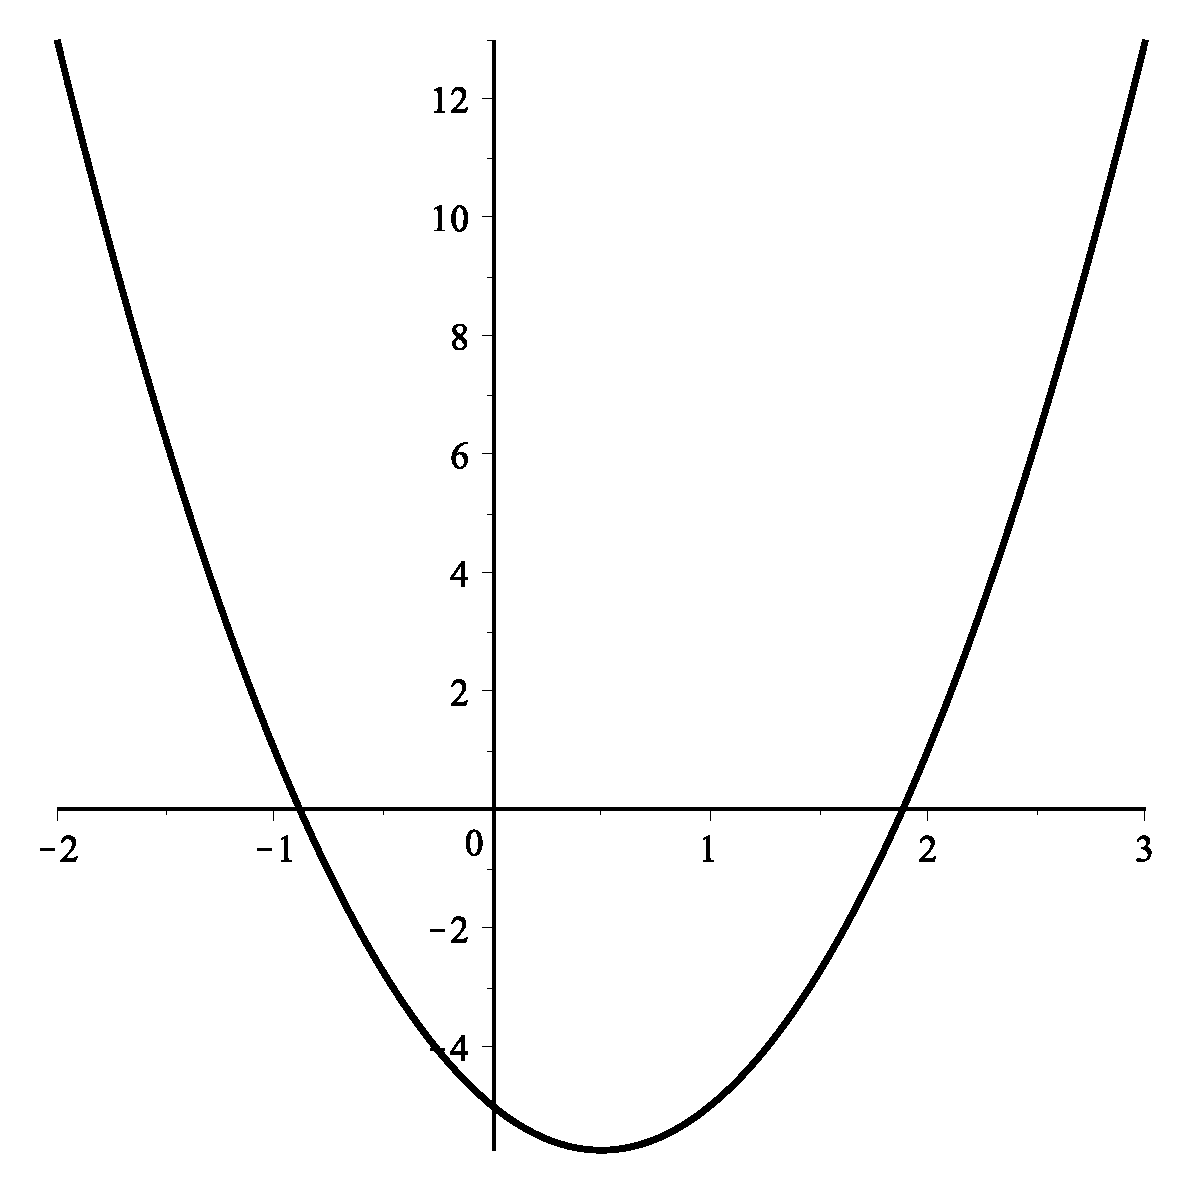
\includegraphics[width=1.5in]{graph_of_general_up_parab}}

{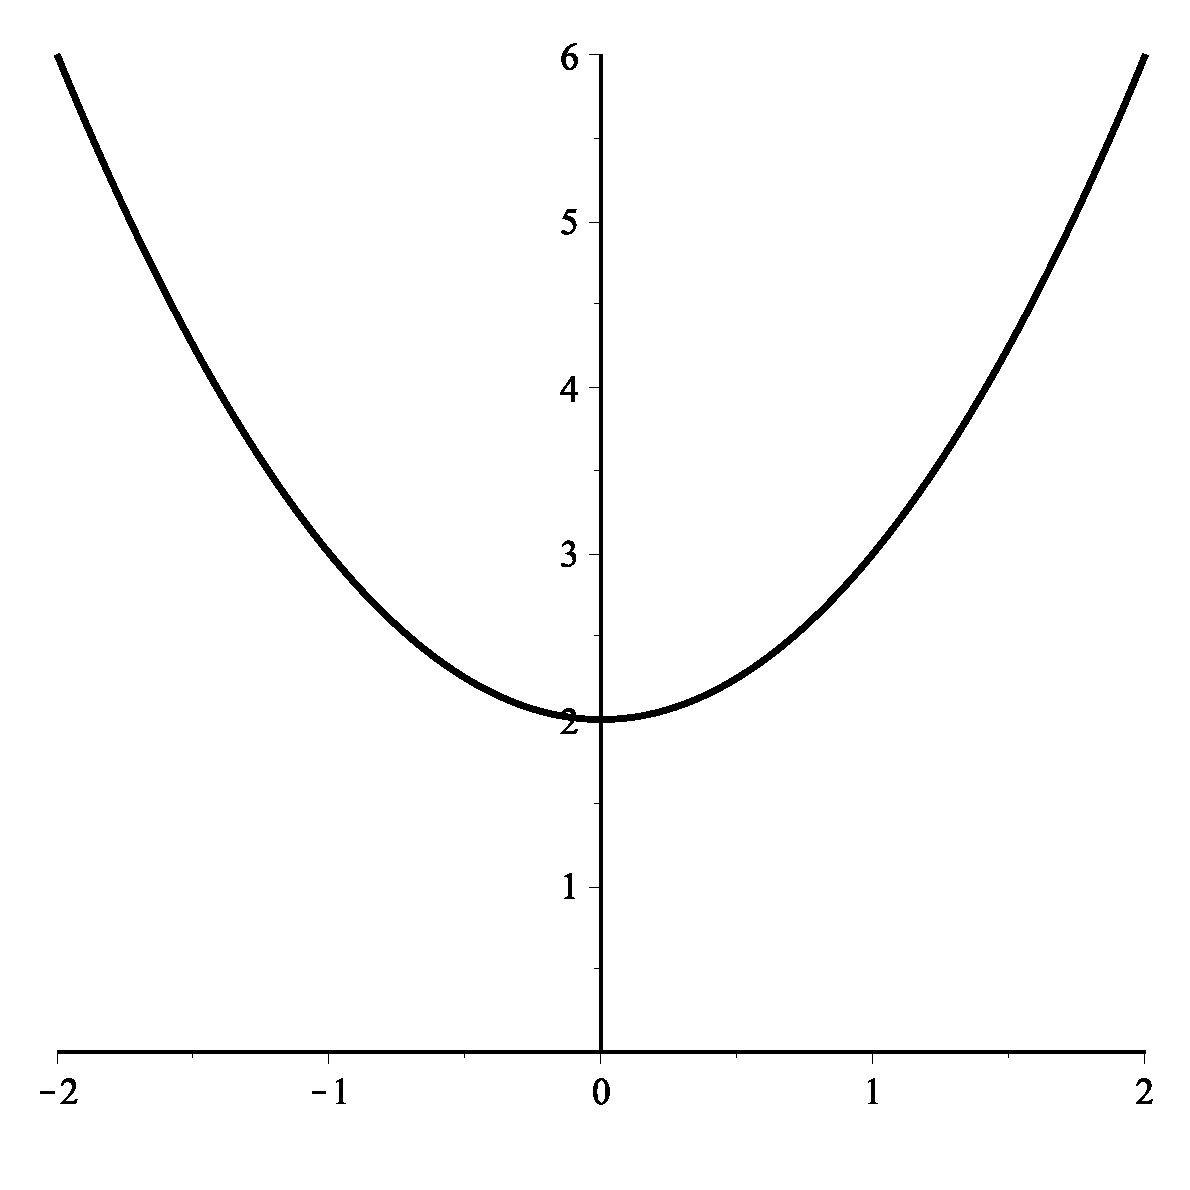
\includegraphics[width=1.5in]{graph_of_x_squared_plus_2}}

{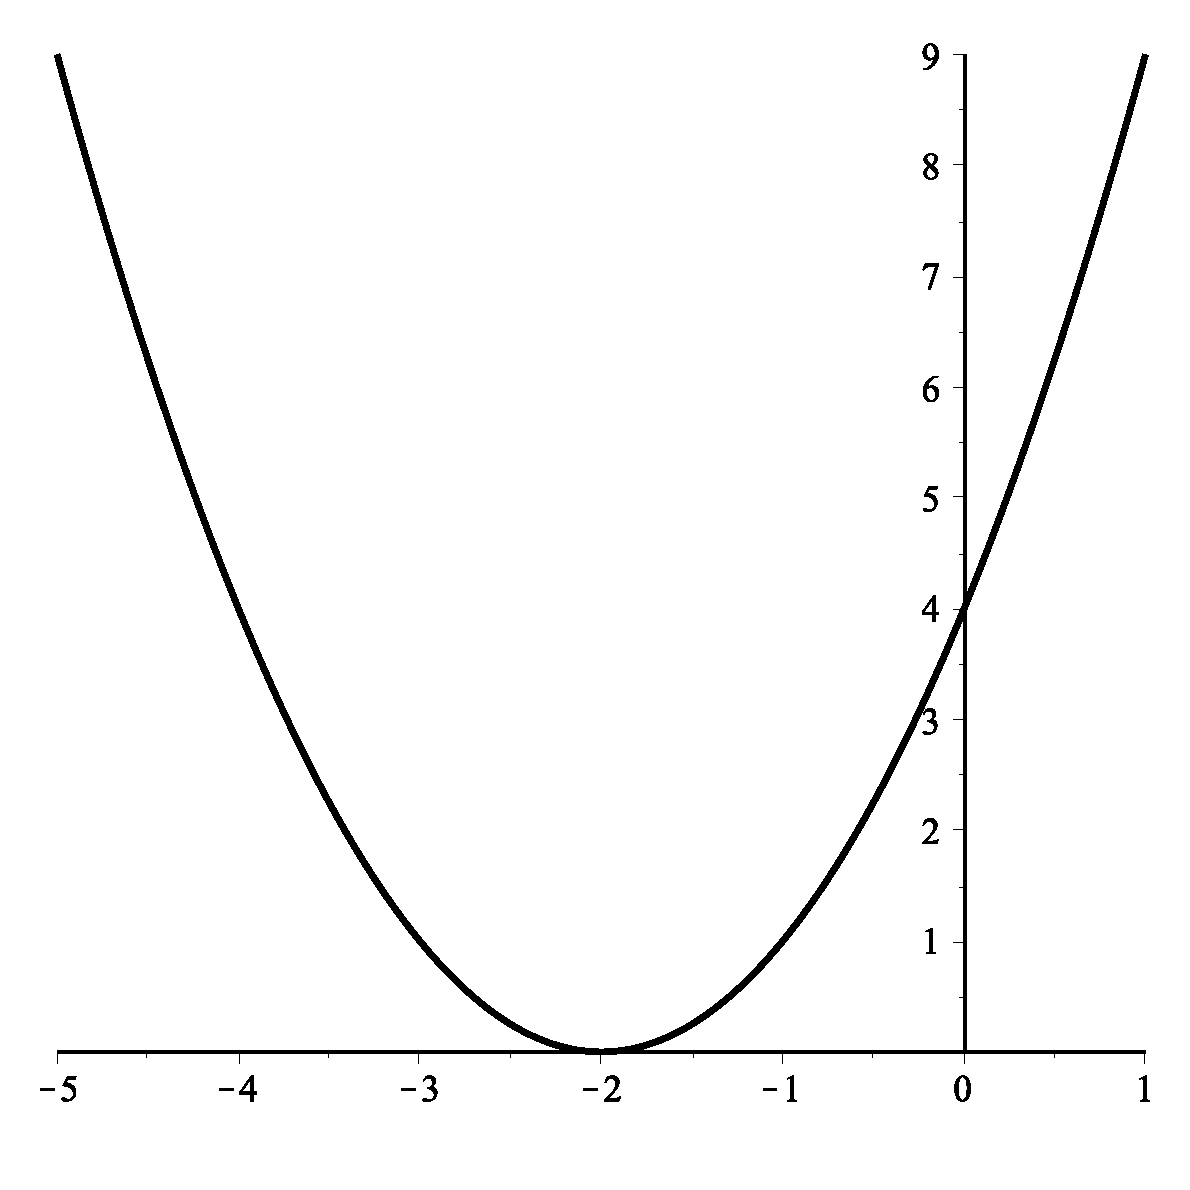
\includegraphics[width=1.5in]{graph_of_x_plus_2_squared}}

{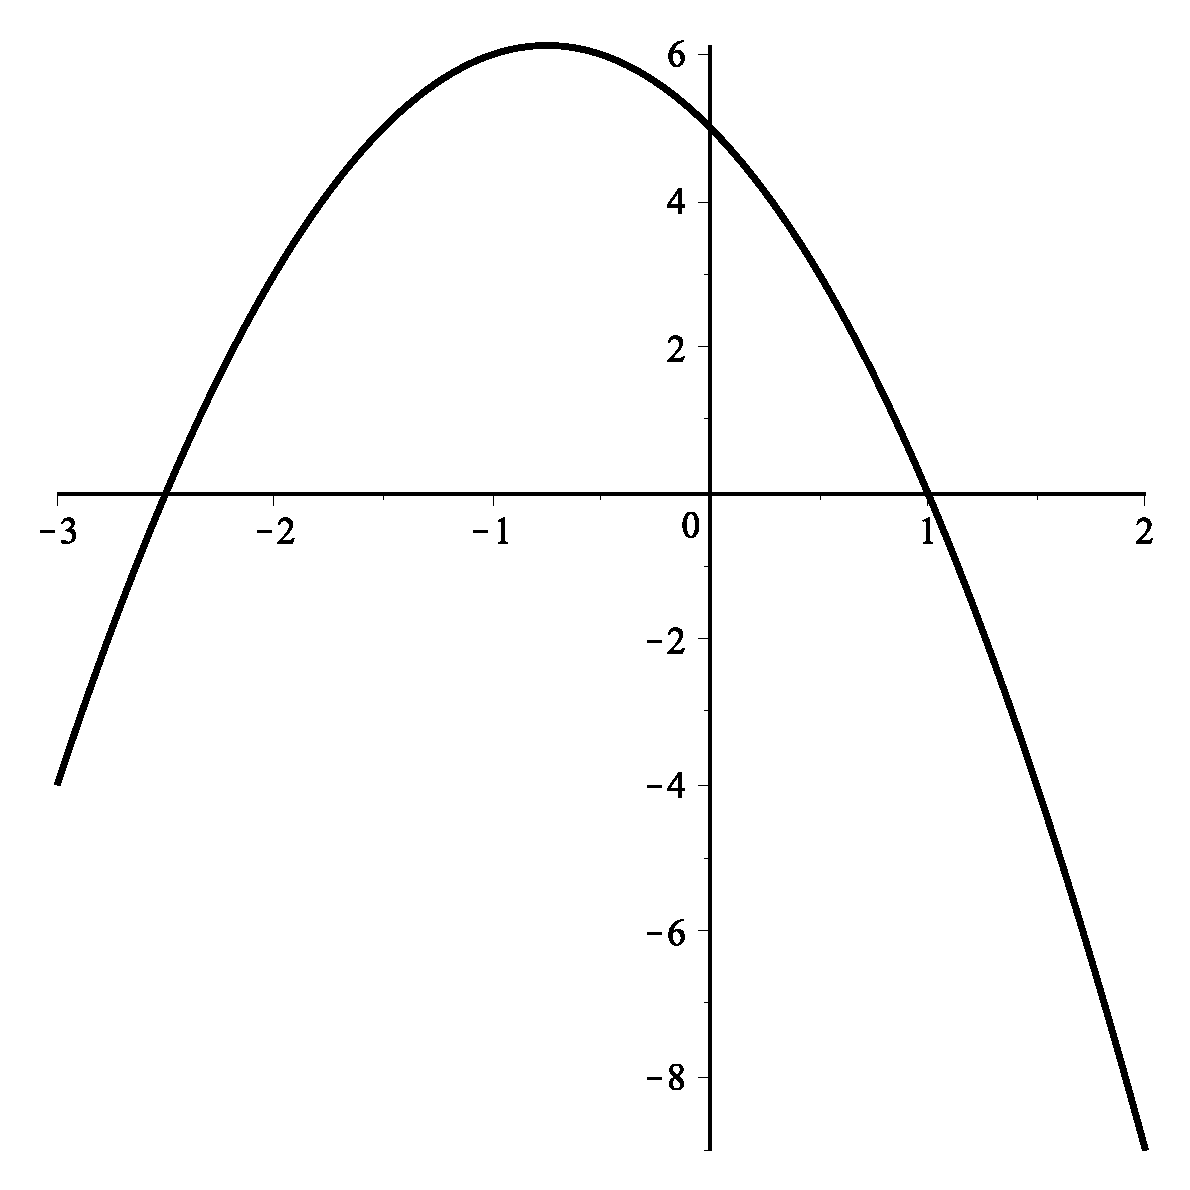
\includegraphics[width=1.5in]{graph_of_general_down_parab}}

{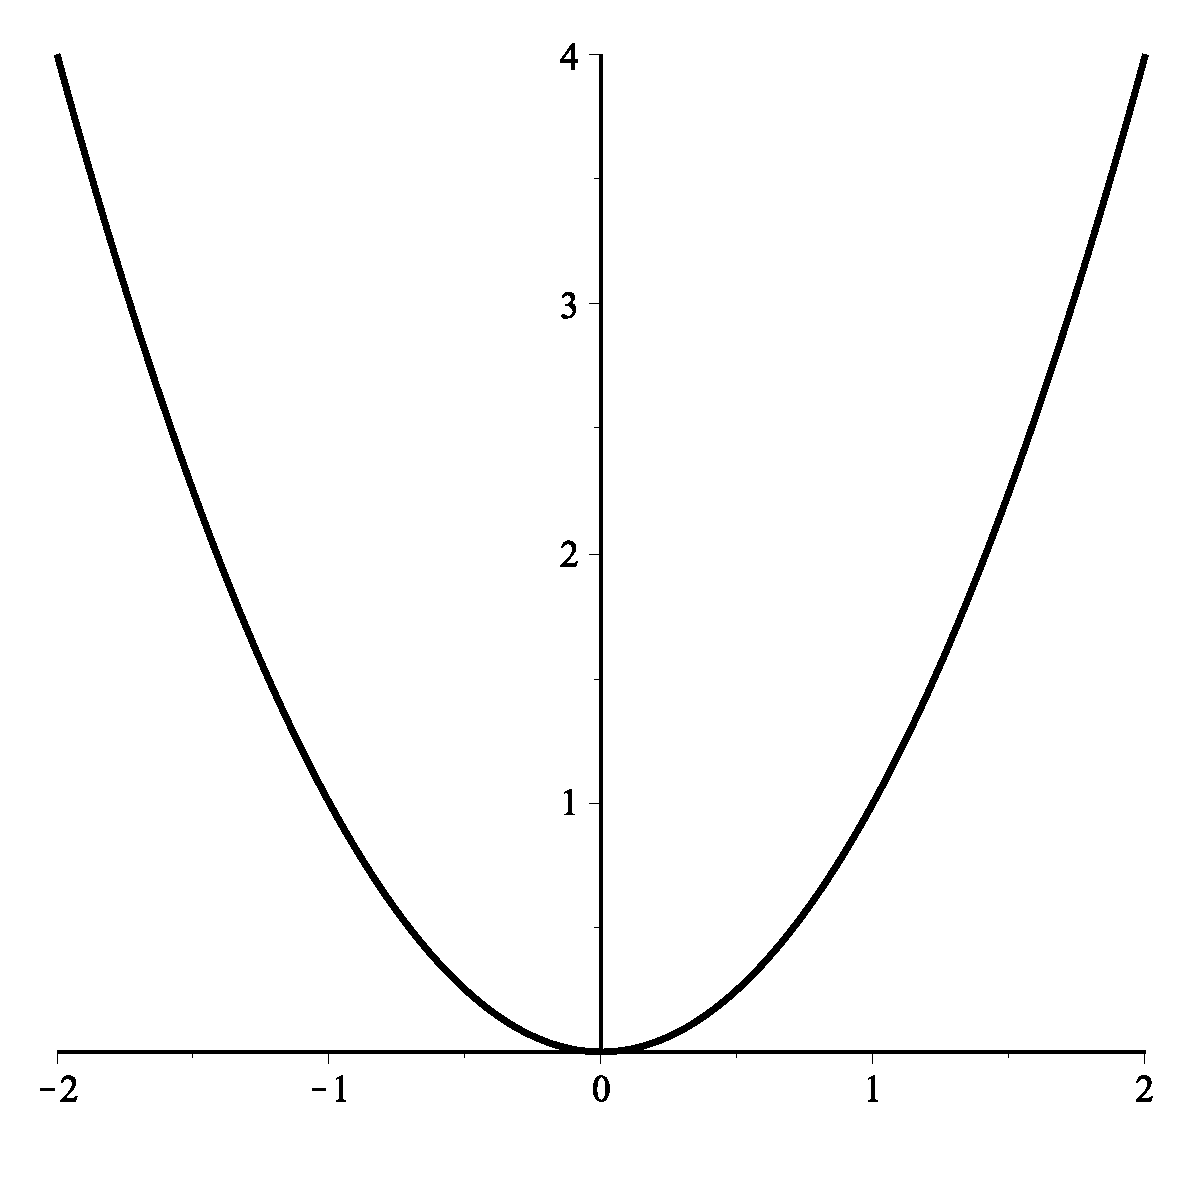
\includegraphics[width=1.5in]{graph_of_x_squared}}
\end{multicols}
\end{beforesolutions}
\end{example}

\begin{solution}\mbox{}
\begin{multicols}{2}
\parskip = 2\bigskipamount

\graphlabel{$3x^2-3x-5$}{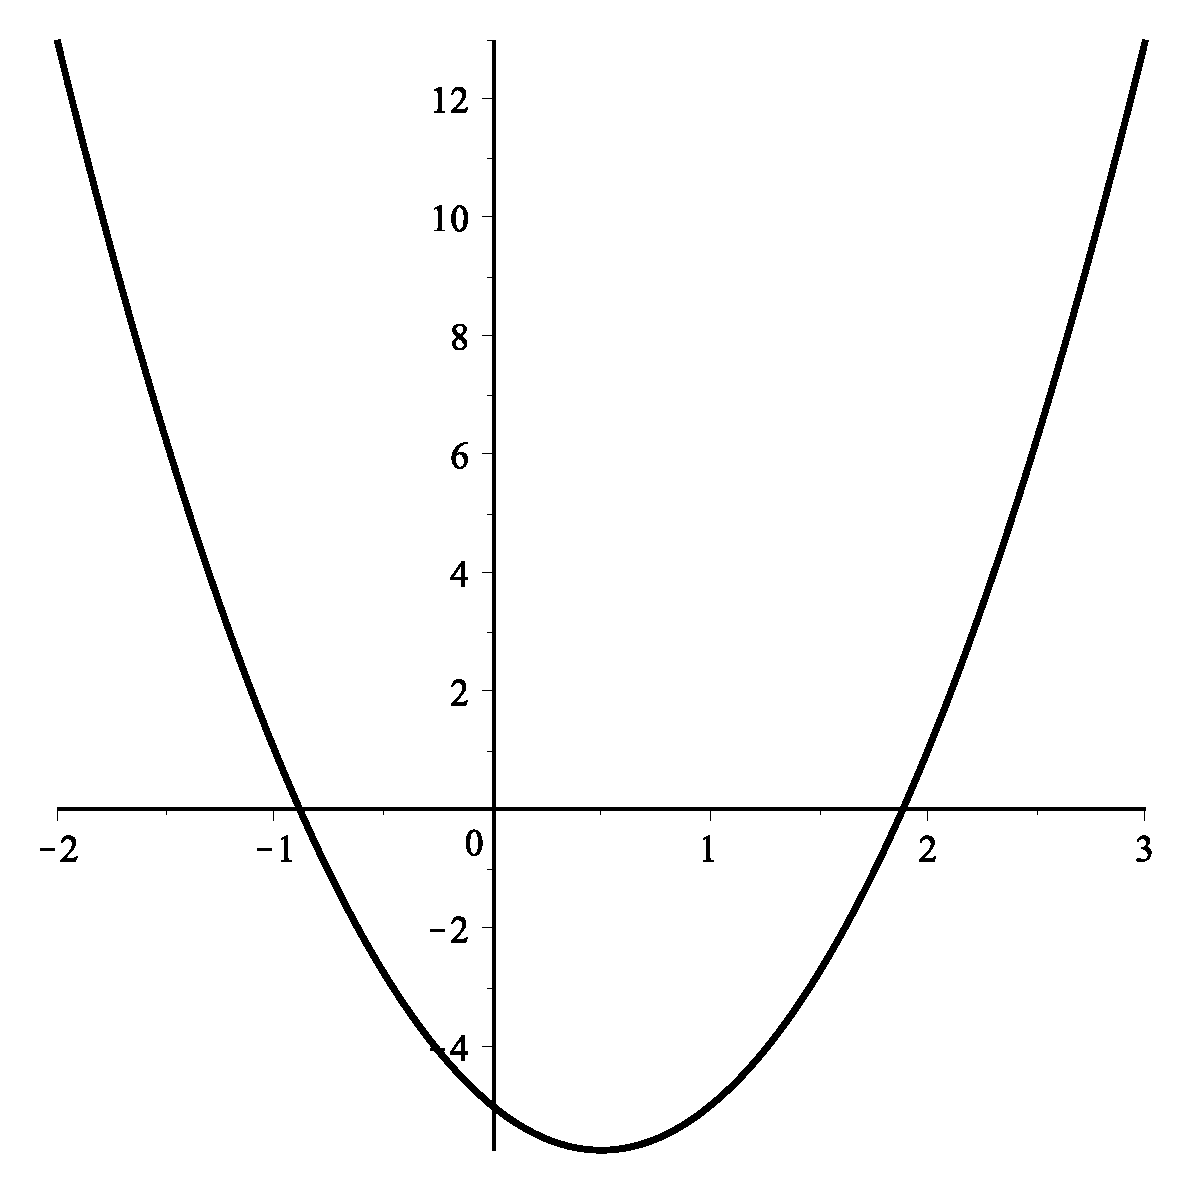
\includegraphics[width=1.5in]{graph_of_general_up_parab}}

\graphlabel{$x^2+2$}{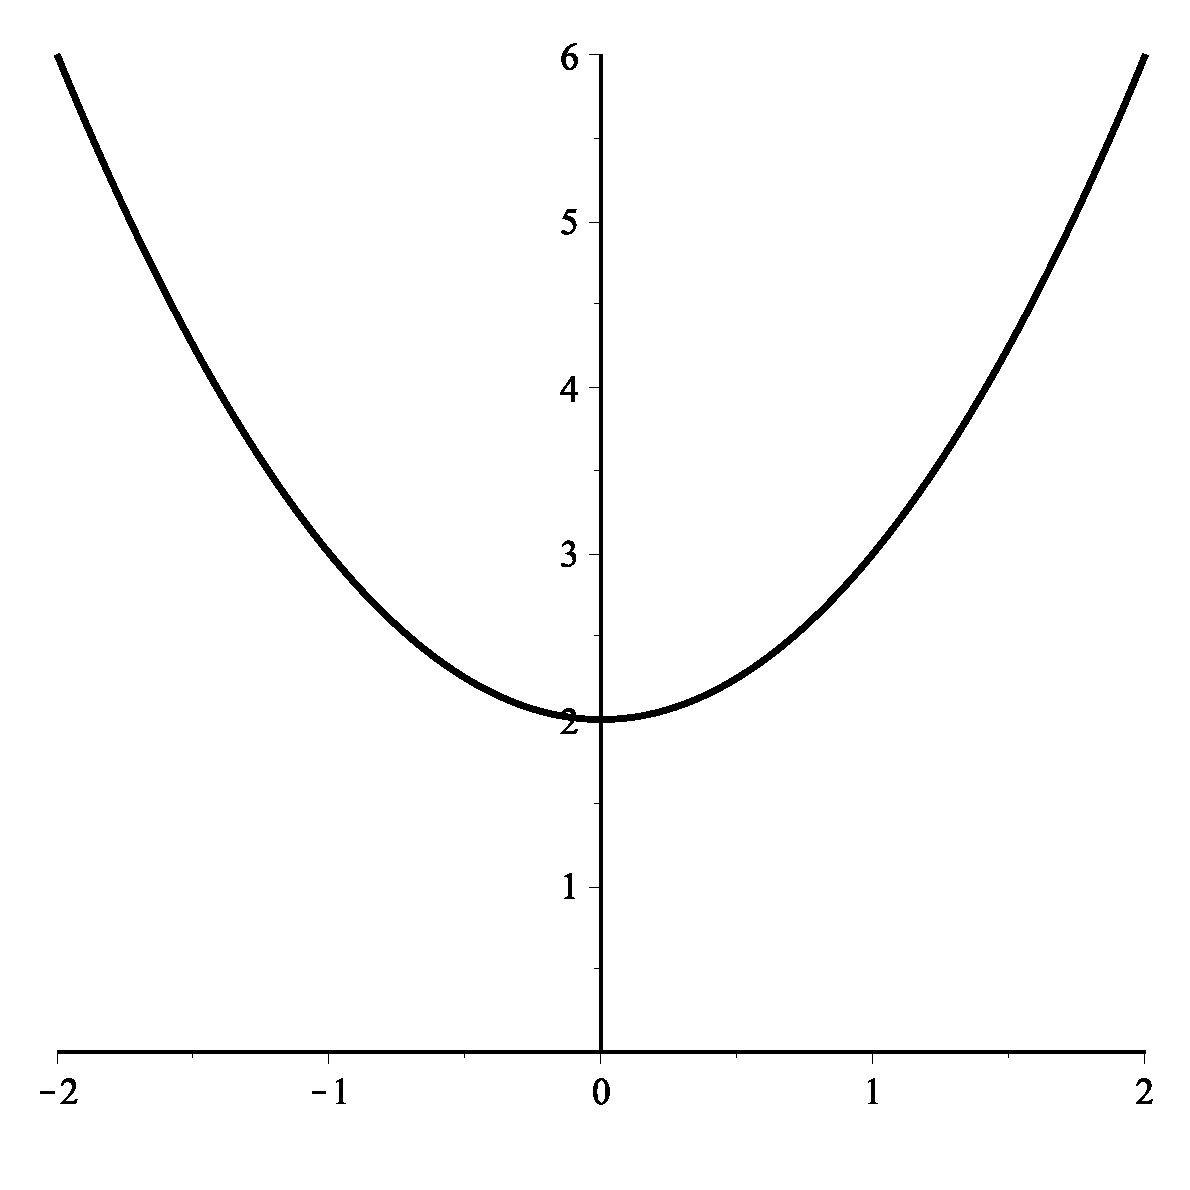
\includegraphics[width=1.5in]{graph_of_x_squared_plus_2}}

\graphlabel{$(x+2)^2$}{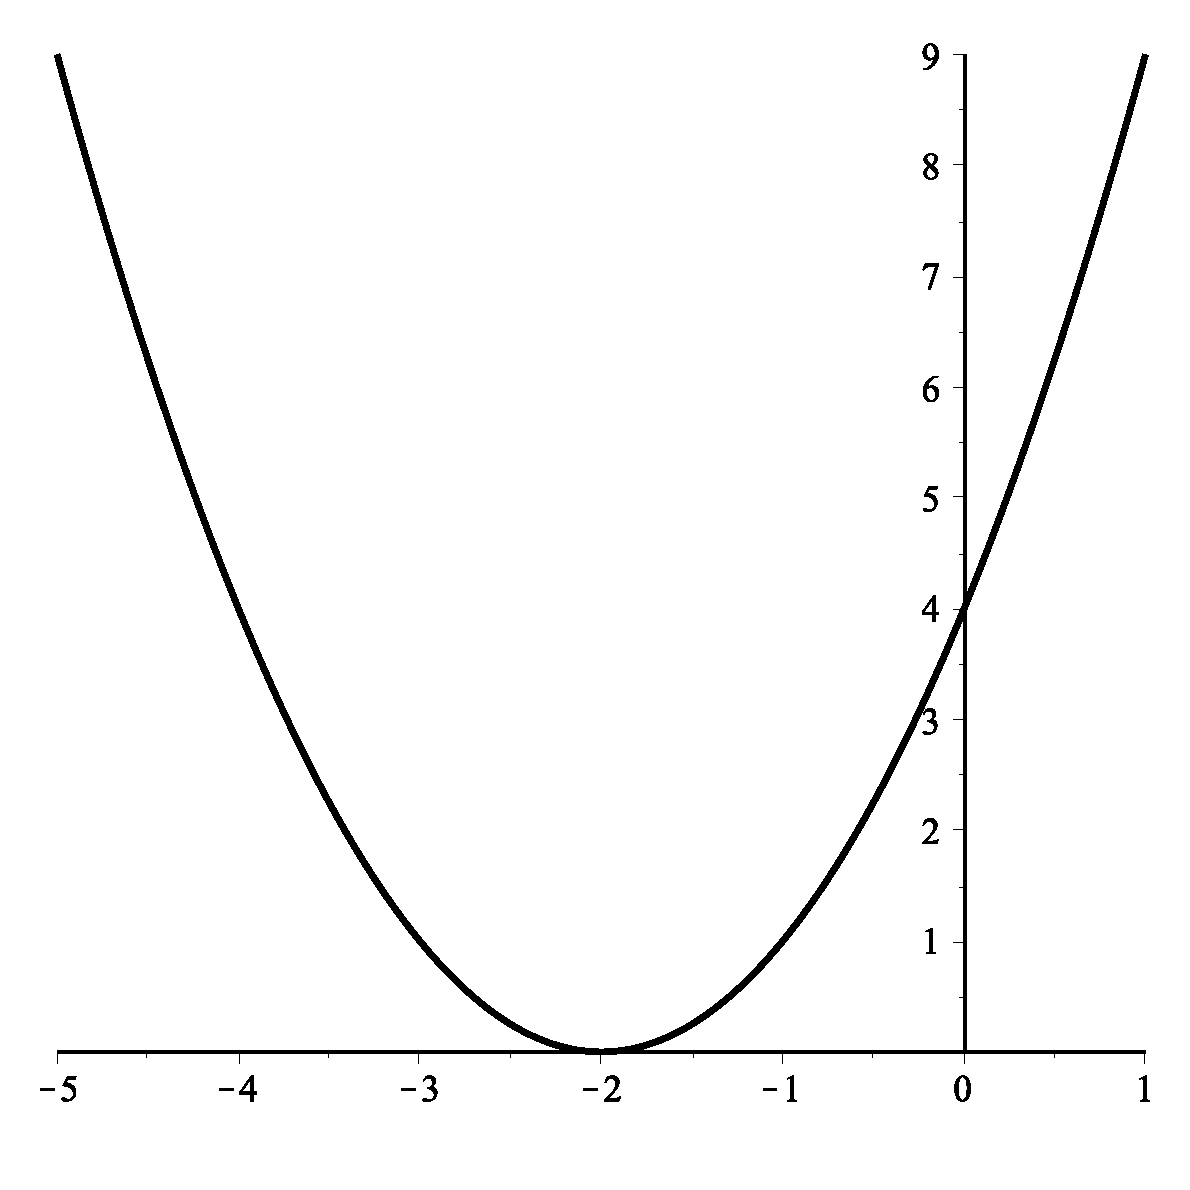
\includegraphics[width=1.5in]{graph_of_x_plus_2_squared}}

\graphlabel{$-2x^2-3x+5$}{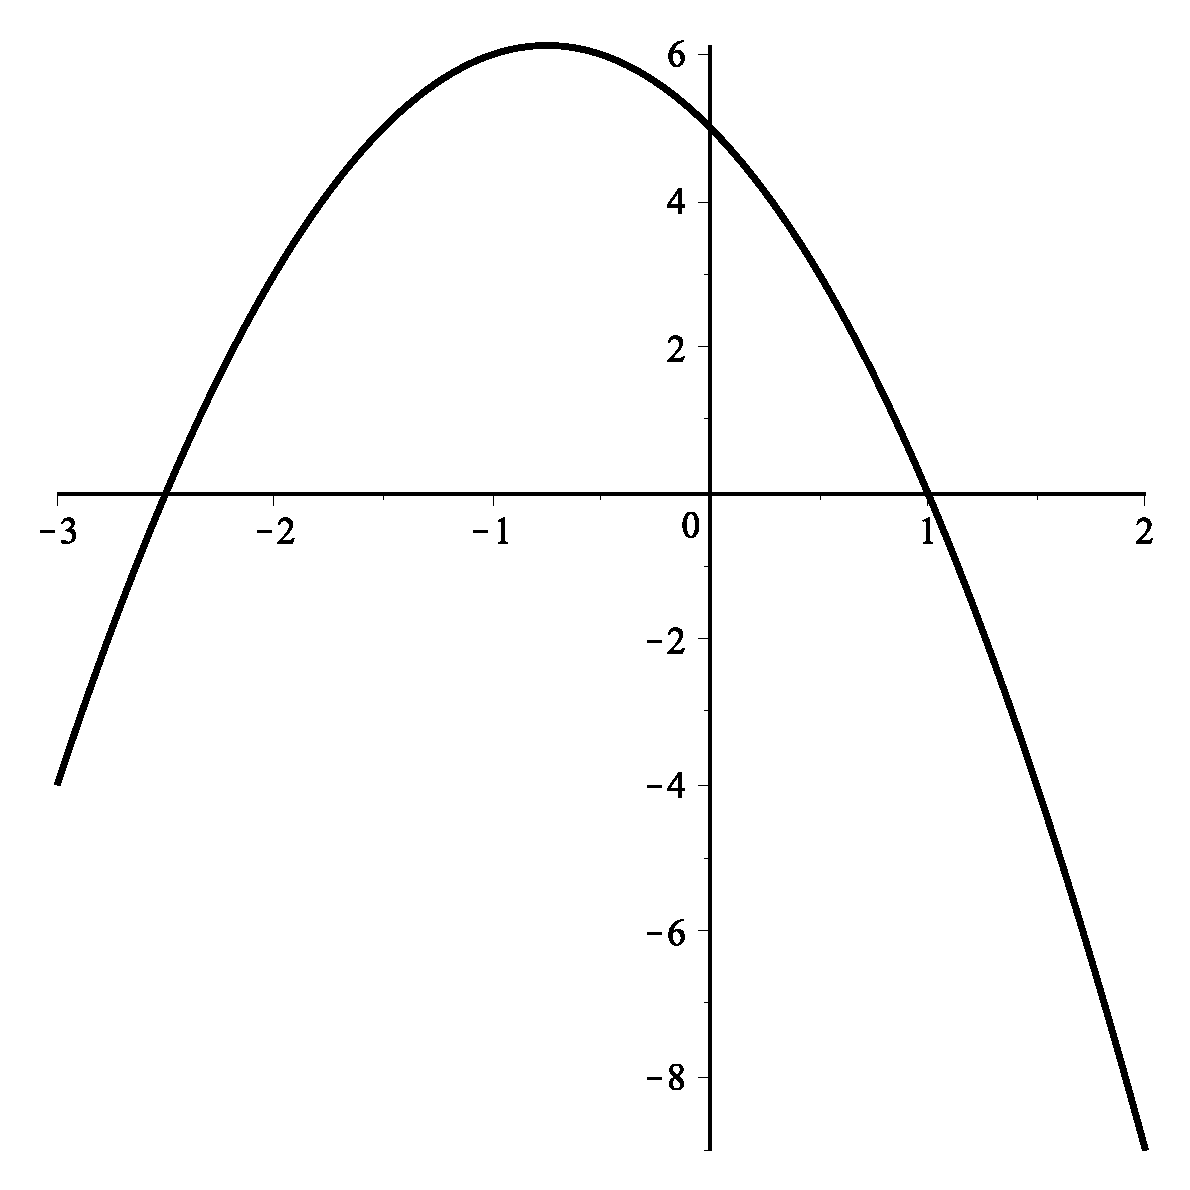
\includegraphics[width=1.5in]{graph_of_general_down_parab}}

\graphlabel{$x^2$}{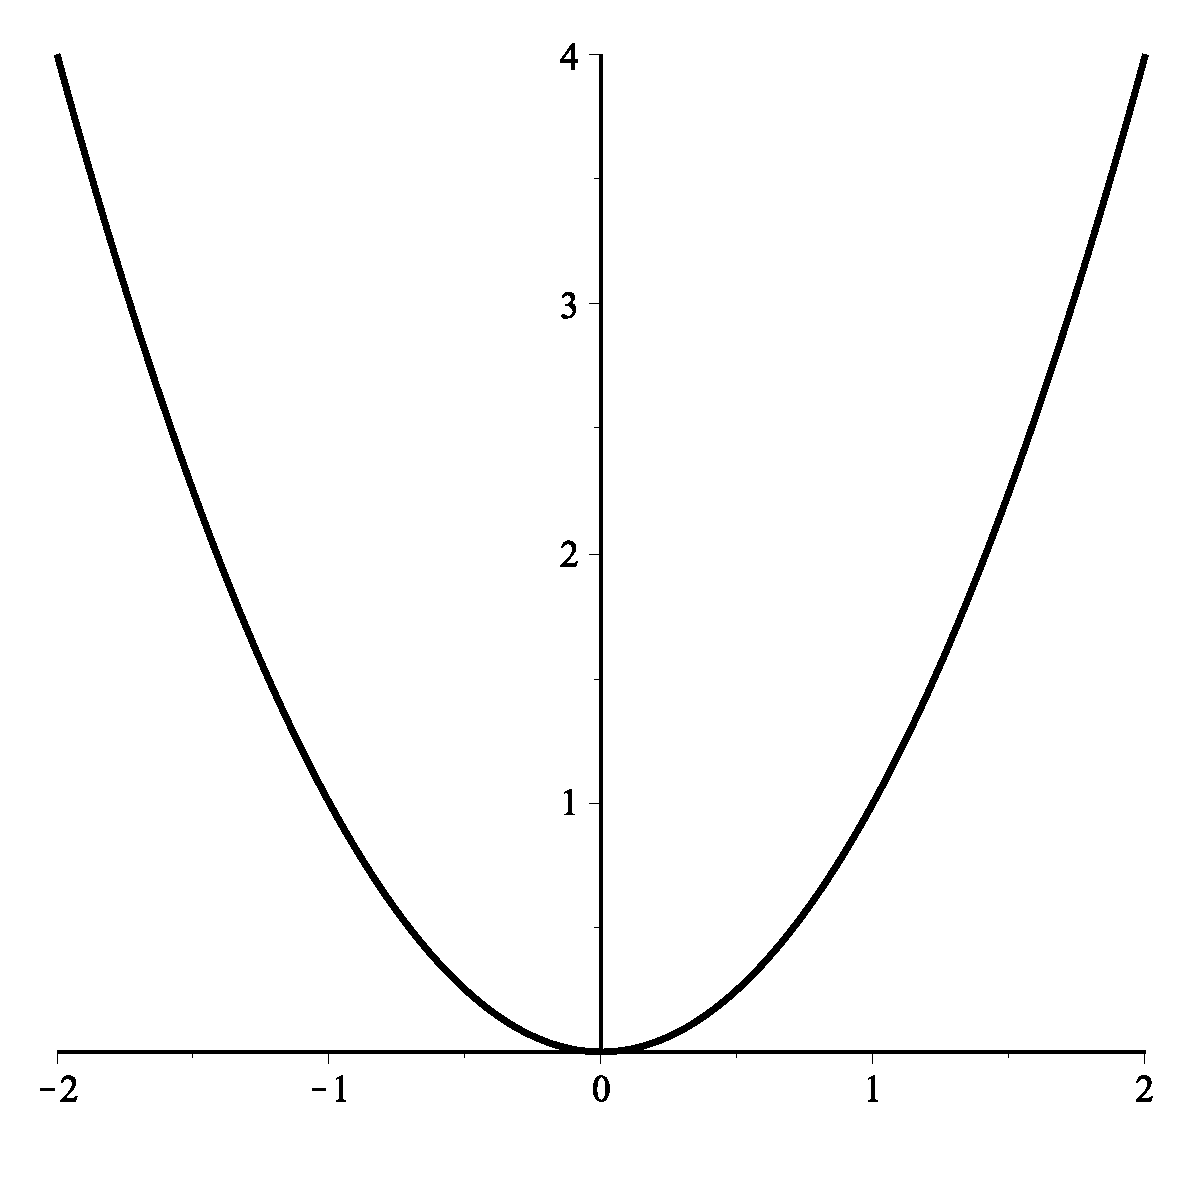
\includegraphics[width=1.5in]{graph_of_x_squared}}

\end{multicols}
\end{solution}




\begin{example}
Factoring a quadratic means to write it as a product.  Usually you
shouldn't bother to factor a quadratic unless the $x^2$-coefficient
equals $1$.  In that case, you're trying to write it like this:
$$
y=x^2+bx+c = (x+d)(x+e)
$$
There are various tricks in finding $d$ and $e$, but honestly, in this
case, I usually just guess and check as follows: (1) guess two values,
$d$ and $e$, that multiply together to give you $c$, and then (2)
check to see if they add up to $b$.  Note: when I write ``$+b$'' and
``$+c$'' and say ``add'' I'm also including negative numbers in there.

\begin{enumerate}
\handoutitemsep
\item Factor and solve $x^2+2x+1=0$.
\item Factor and solve $x^2+3x+2=0$.
\item Factor and solve $x^2-3x+2=0$.
\item Factor and solve $x^2-x-2=0$.
\item Factor and solve $x^2-x-12=0$.
\item Factor and solve $x^2-8x+12=0$.
\handoutfill
\end{enumerate}
\end{example}

\begin{solution}
\begin{multicols}{2}
\begin{enumerate}
\item \begin{align*}
x^2+2x+1 & =0\\
(x+1)(x+1) & = 0\\
x& = -1
\end{align*}

\item 
\begin{align*}
x^2+3x+2 & = 0\\
(x+2)(x+1) & = 0\\
x & = -2, -1
\end{align*}

\item
\begin{align*}
x^2-3x+2 & = 0\\
(x-2)(x-1) & = 0\\
x & = 1,2
\end{align*}

\item
\begin{align*}
x^2-x-2 & = 0\\
(x-2)(x+1) & =0\\
x & = -1,2
\end{align*}

\item
\begin{align*}
x^2-x-12 & = 0\\
(x-4)(x+3) & = 0\\
x & = -3,4
\end{align*}

\item
\begin{align*}
x^2-8x+12 & = 0\\
(x-10)(x+2) & = 0\\
x=-2,10
\end{align*}
\end{enumerate}
\end{multicols}
\end{solution}



\begin{example}
  A lot of times it's not worth factoring a quadratic, or it may be
  impossible.  In these cases, just use the quadratic formula
$$
ax^2+bx+c = 0 
\quad \Longrightarrow \quad 
x = \frac{-b\pm \sqrt{b^2-4ac}}{2a}
$$
\begin{enumerate}
\handoutitemsep
\item Apply the quadratic formula to $x^2-x-12=0$.
\item Apply the quadratic formula to $2x^2+3x-2=0$.
\handoutfill
\end{enumerate}
\end{example}

\begin{solution}
\begin{enumerate}
\item 
\begin{align*}
x & = \frac{+1 \pm \sqrt{(-1)^2 -4(1)(-12)}}{2(1)}\\
  & = \frac{1 \pm \sqrt{1+48}}{2}\\
  & = \frac{1 \pm \sqrt{49}}{2}\\
  & = \frac{1 \pm 7}{2}\\
  & = \frac{8}{2}, \frac{-6}{2}\\
  & = 4, -3
\end{align*}
(Note: this is the same as part (e) in the previous example.)

\item 
\begin{align*}
x & = \frac{-3 \pm \sqrt{(3)^2 -4(2)(-2)}}{2(2)}\\
  & = \frac{-3 \pm \sqrt{9+16}}{4}\\
  & = \frac{-3 \pm \sqrt{25}}{4}\\
  & = \frac{-3 \pm 5}{4}\\
  & = \frac{2}{4}, \frac{-8}{4}\\
  & = 1/2, -2
\end{align*}
\end{enumerate}
\end{solution}


\chapter{Functions and Change}
%%%%%% Section 1.1
\section{What is a Function?}

\begin{example}
\begin{enumerate}
\item $f(x) = x^2$, then $f(5) = ?$
\item $g(t) = \sqrt{t^2 + 1}$, \qquad $g(0) = ?$, \qquad $g(-3) = ?$
\item $f(t+1) = ?$
\item $g(x + h) = ?$
\end{enumerate}
\end{example}

\begin{solution}
\begin{enumerate}
\item In the formula ``\,$f(x)=x^2$\,'' we simply replace each ``$x$''
  with $5$ to get
$$
f(5) = 5^2
$$
Maybe that's the best place to stop, because this problem isn't really
about calculating $5^2$ it's about how we combine $x^2$ and $5$, which
we've done.  But I know the curiosity is killing you, so we can go to
the next step and say:
$$
f(5) = 5^2 = 25
$$

\item With a little practice, you should be able to find $g(0)$ in
  your head, but for now, let's write out every step:
\begin{align*}
g(0) & = \sqrt{0^2 + 1}\\
     & = \sqrt{1}\\
     & = 1
\end{align*}
For $g(-3)$ the only real difference is that you should be careful
about order of operations with the negative $3$.  Note that whatever
we plug in for $t$ should be squared, including the negative:
\begin{align*}
g(-3) & = \sqrt{(-3)^2 + 1}\\
     & = \sqrt{9+1}\\
     & = \sqrt{10}
\end{align*}
We'll leave the answer in this form, because the point of this example
\emph{isn't} how to find the square root using our calculator.  The
point is do we know where to put the $-3$.

\item For $f(t+1)$ it might help if we first write $f$ without using
  $x$.  Remember, ``$x$'' is just a letter we use to stand for
  something else.  If you get too fixated on $x$ you might miss how
  $f$ is really defined, and therefore how to find $f(t+1)$.  Here's a
  different way to write $f$:
$$
f(\quad) = (\quad)^2
$$
Whatever you put into $(\quad)$ on the left you should also put into
$(\quad)^2$ on the right:
$$
f(t+1) = (t+1)^2
$$
I'll stop there for (c) because the point isn't whether we can FOIL or
expand $(t+1)^2$, the point is did we plug $t+1$ in correctly.

\item As in the last part, let's first write $g$ without using the
  letter $t$, just using a blank space which we can plug stuff into:
$$
g(\quad)=\sqrt{(\quad)^2+1}
$$
Now, we should plug $x+h$ into $(\quad)$ on both the left and the
right:
$$
g(x+h)=\sqrt{(x+h)^2+1}
$$
Again, I won't try to expand and rewrite that any, because it's not
the point, and because in this problem it doesn't really help.
\end{enumerate}
\end{solution}

\begin{example}
  The historic Senator Theater is the nearest movie theater to Loyola.
  Their ticket prices for adults (non-students) seeing a 3D movie are
  \$13.50 for movies after 6 PM, \$11 for a matinee (noon -- 6 PM),
  and \$9 for an early bird show (before 11 AM).  Write a piecewise
  function $P(t)$ for the price of the ticket where $t$ is the time of
  the showing.
\end{example}

\begin{solution}
  Basically we're just taking the given information about pricing and
  times and arranging it using the notation for piecewise functions.
  We put the prices first, and then times second.  (In general we put
  formulas first, and the conditions second.)  In this case we get
$$ 
P(t) = 
\begin{cases}
9 & \text{ if }t< 11:00\\
11 & \text{ if }12:00 \le t \le 18:00\\
13.50 & \text{ if }t> 18:00
\end{cases}
$$
\end{solution}

\begin{example}
  Since July 1, 2016, the Maryland minimum wage is \$8.75 per hour
  (FYI: it will increase to \$9.25 on July 1, 2017).  Suppose someone
  is able to make time and a half per hour of overtime (over 40
  hours).  If $x$ is the number of hours worked for this week and
  $f(x)$ is the income function for (gross) income earned that week,
  answer the following:

\begin{enumerate}
\item Make up an integer $A$ such that $A<40$, and then calculate $f(A)=$?
\item Make up an integer $B$ such that $B>40$, and then calculate $f(B)=$?
\item Make up a non-integer $C$ that $C<40$, and then calculate
  $f(C)=$? (For instance, $f(10.5)=?$)
\item Make up a non-integer $D$ that $D>40$, and then calculate $f(D)=$?
\item $f(x) = $? in general
\end{enumerate}
\end{example}

\begin{solution} 
(e) Time and a half rate is $8.75(1.5) = 13.125$
$$
I(x) = 
\begin{cases} 
  8.75 x & \text{ if }x \le 40\\ 
  8.75\cdot 40 + 13.125(x-40) & \text{ if }x > 40 
\end{cases}
$$
\end{solution}

\begin{example}
What are the domains of these functions?
\begin{enumerate}
\item $f(x) = 3x-5$
\item $g(x) = \sqrt{x+5}$
\item $h(x) = \dfrac{1}{x}$
\item $F(t) = \dfrac{\sqrt{5-t}}{t+2}$
\end{enumerate}
\end{example}

\begin{solution}
  The domain is the set of all numbers that we can plug into our
  formula.  When I say ``we can plug in'' I mean so that the result is
  defined, or calculate-able.  The way we find the domain is to look
  for the numbers that are not in it, the numbers that make things
  undefined or un-calculate-able.  In other words, we look for the
  problem spots.

  With algebraic functions like these there are only two possible
  kinds of problem spots: division by 0, and square roots of negative
  numbers.  These are problems, and so these are not in the domain.

\begin{enumerate}
\item For $3x-5$ are there any problem spots?  Is there any number I
  could plug in that would lead to division by $0$ or the square root
  of a negative number?  No.  There is no division, and there is no
  square root here.

  No problem spots means that all numbers are ok.  Thus, the domain is
  all real numbers.  We write this in two ways:
$$
\begin{array}{ccc}
\text{interval notation} & & \text{inequalities}\\
(-\infty,\infty)  && \infty < x < \infty
\end{array}
$$


\item For $\sqrt{x+5}$ are there are problem spots?  Is there any
  number I could plug in that would lead to division by $0$ or the
  square root of a negative number?  No for division, yes for the
  square root of a negative number.
\begin{align*}
\sqrt{x+5} & \text{ needs}\\
x+5 & \ge 0\\
x & \ge -5
\end{align*}
Again, these are the numbers that are ok, i.e.\ that are in the
domain.

As before, we write this in two ways:
$$
\begin{array}{ccc}
\text{interval notation} & & \text{inequalities}\\
(-5,\infty) &&  x \ge -5
\end{array}
$$

\item For $\frac 1x$ are there are problem spots?  Is there any number
  I could plug in that would lead to division by $0$ or the square
  root of a negative number?  No for square roots, yes for division.
\begin{align*}
\frac 1x & \text{ needs}\\
x & \ne 0
\end{align*}
Again, these are the numbers that are ok, i.e.\ that are in the domain. 

As before, we write this in two ways:
$$
\begin{array}{ccc}
\text{interval notation} & & \text{inequalities}\\
(-\infty,0)\cup (0,\infty) && x \ne 0
\end{array}
$$

\item For $\frac {\sqrt{5-t}}{t+2}$ are there are problem spots?  Is
  there any number I could plug in that would lead to division by $0$
  or the square root of a negative number?  Yes for both!
\begin{align*}
\sqrt{5-t} & \text{ needs}\\
5-t  & \ge 0\\
5 & \ge t\\
t & \le 5\\
\frac{\text{something}}{t+2} & \text{ needs}\\
t+2 & \ne 0\\
t & \ne -2
\end{align*}
Again, these are the numbers that are ok, i.e.\ that are in the domain. 

We need both of these conditions to be true: $t\le 5$ and $t\ne -2$.
This is a good way to write the answer, but if we want to make it look
like the other answers, then we can write this in two ways:
$$
\begin{array}{ccc}
\text{interval notation} & & \text{inequalities}\\
(-\infty,-2)\cup (-2,5) &  & t <-2 \text{ or }-2 < t \le 5
\end{array}
$$
\end{enumerate}
\end{solution}

%%%%%% Section 1.2
\section{Linear Functions}


\begin{example}
  For the two points $(1,2)$ and $(-5,4)$ what is the slope of the
  line connecting them?
\end{example}
 
\begin{solution}
There are probably three useful ways to think about the slope
\begin{align*}
m & = \frac{\text{rise}}{\text{run}}\\
  & = \frac{y_2-y_1}{x_2-x_1}\\
  & = \frac{\Delta y}{\Delta x}
\end{align*}
Note that all three of these formulas say the same thing: ``rise''
really means $y_2-y_1$, i.e.\ how much did $y$ change.  Similarly,
``$\Delta y$'' is just shorthand notation for ``change of $y$''.

The main things you have to watch out for in this kind of problem are:
(1) make sure you put the $y$'s on top, (2) make sure you use the
numbers in the same order on the top and bottom.  Here's a picture of
how the numbers should move into the correct places:
\begin{center}
\begin{tikzpicture}[
  every node/.style={inner sep=2pt},
  lasso/.style={shape=ellipse, draw}
% the ellipse can be tweeked with xscale, yscale, inner xsep and inner ysep
]
\path (-1.25,3.25) node[left]{
$\begin{array}{rl}
\multicolumn{2}{r}{\text{Given Points}}\\
(-5, & 4)\\
(1, &  2)
\end{array}$};

\path (0,1) node (x1) {\llap{$-$}$5$};
\path (1,1) node (y1) {$4$};
\path (0,0) node (x2) {$1$};
\path (1,0) node (y2) {$2$};

\path (x1) node[left=0.75cm] {1st in subtraction};
\path (x2) node[left=0.75cm] {2nd in subtraction};
\path (x1) ++ (0,1.25) node[right,rotate=90] {top of fraction};
\path (y1) ++ (0,1.25) node[right,rotate=90] {bottom of fraction};

\begin{scope}[xshift=7cm]
\path (0,1) node (n1) {$4$};
\path (1,1) node (n2) {$2$};
\path (0,0) node (d1) {\llap{$-$}$5$};
\path (1,0) node (d2) {$1$};
\path (0.5,1) node {$-$};
\path (0.5,0) node {$-$};
\draw (-0.5,0.5) -- (1.5,0.5);
\end{scope}

\begin{scope}[color=red!75!black,very thick]
\node[fit=(x1)(x2), lasso] (Ltop) {};
\node[fit=(y1)(y2), lasso] (Lbot) {};
\node[fit=(n1)(n2), lasso] (Rtop) {};
\node[fit=(d1)(d2), lasso] (Rbot) {};
\draw[->,out=35,in=180,shorten >=5pt] (Ltop.north) to (Rtop.west);
\draw[->,out=25,in=180,shorten >=5pt] (Lbot.north) to (Rbot.west);
\end{scope}

\begin{scope}[color=green!65!black,very thick]
\node[fit=(x1)(y1), lasso] (L1st) {};
\node[fit=(x2)(y2), lasso] (L2nd) {};
\node[fit=(n1)(d1), lasso] (R1st) {};
\node[fit=(n2)(d2), lasso] (R2nd) {};
\draw[->,out=-25,in=240,shorten >=5pt] (L1st.east) to (R1st.south);
\draw[->,out=-35,in=270,shorten >=5pt] (L2nd.east) to (R2nd.south);
\end{scope}
\end{tikzpicture}
\end{center}
Now we finish our calculation:
\begin{align*}
 m & = \frac{4 - 2}{-5 - 1}\\
   & = \frac{\ 2\ }{-6}\\
   & = - \frac 13
\end{align*}
\end{solution}

%DRAW SOME LINES/EQUATIONS - GOOD OPPORTUNITY FOR MATCHING QUIZ OR SOMETHING

%\begin{example}{1.2 Example 2: Problem 10}
%  \begin{enumerate}[(a)]
%  \item Which two lines in Figure 1.22 have the same slope?  Of these two lines, which has the larger $y$-intercept?
%  \item Which two lines have the same $y$-intercept? Of these two lines, which has the larger slope?
%  
%  \mygraphcentered{0.5\textwidth}{Images/s1-2prob10}
%  \end{enumerate}
%\end{example}
%


\begin{example}
  Find an equation of the line that passes through $(1,2)$ and
  $(-5,4)$.
\end{example}

\begin{solution}
  We'll start with the point-slope form of the equation of a line:
   $$
   y  = m(x-x_0) + y_0\\
  $$
  From Example 1, we know the slope already, $m = -\frac{1}{3}$.  Then
  we can use either $(1,2)$ or $(-5,4)$ for the known point.  We'll
  use $(1,2)$.
$$
          y = -\frac{1}{3}(x-1) +2
$$
There's nothing wrong with leaving the equation like this, but most of
us are more used to the slope-intercept form, so we can distribute the
numbers and simplify:
  \begin{align*}
    y & = -\frac{1}{3}x + \frac{1}{3} + 2 \\
    y  & = -\frac{1}{3}x + \frac{1}{3} + \frac{6}{3}\\
    y  & = -\frac{1}{3}x + \frac{7}{3}
  \end{align*}
\end{solution}

\begin{example}
  A cab company has an initial charge of $\$4.00$ plus $\$2.20$ per
  mile.  Find a formula for the cab fare, $C$, in dollars, as a
  function of the number of miles, $m$.
\end{example}


\begin{solution}
  There are three things to identify here: where do we put the $4.00$,
  where do we put the $2.20$, and which variables should we use?

  The $4.00$ is the initial charge.  The word ``initial'' means at the
  very beginning, in this case, before we start driving at all.  This
  means it's the value when we've gone $0$ miles, which is another way
  to say it's the $y$-intercept, or the vertical intercept.

  The $2.20$ is a charge \underline{\ per\ }mile.  The word ``per'' is a
  clue that this is the slope: slope is a ratio, and ``per'' always
  means ratio too.

  Putting these together we should have
$$
\text{something like }y = 2.20\times \text{something like }x + 4.00
$$
The correct somethings are $C$ instead of $y$ and $m$ instead of $x$.
I know it looks weird, but ``$m$'' is our variable here, not slope
(since $m$ looks so weird, that's why I wrote it out with words first,
to make sure I got things in the right place).
  $$ 
  C = 2.20m + 4
  $$
\end{solution}


\begin{example}
  ACME company has seen a decline in sales of their product. In 2010
  they sold 28.4 million, while in 2016 they sold 22.7 million.
  \begin{enumerate}
  \item Find a formula for annual sales $S$, in millions of items, as
    a linear function of the years $t$, since 2010.
  \item Predict the sales in 2019.
  \end{enumerate}
\end{example}

\begin{solution}
  \begin{enumerate}
  \item We have two points of the line: $(0, 28.4)$, and $(6, 22.7)$, which gives us
    $$ 
    m = \frac{22.7-28.4}{6-0} = \frac{-5.7}{6} = -0.95
    $$
    Luckily, we were given the $y$-intercept of $28.4$ so we have
    $$ 
    S(t) = -0.95t + 28.4
    $$
  \item Use $t = 9$ to get
    $$ 
    S(9) = -0.95(9) + 28.4 = 19.85
    $$
    Thus we predict sales of $19.85$ million in the year 2019.
  \end{enumerate}
  \end{solution}

%%%%%% Section 1.3
\handoutpagebreak

\section{Rates of change}
\begin{example}[Problem 12]
  Table 1.14 shows world bicycle production (from
  \url{http://www.earth-policy.org/indicators/C48/},
  accessed April 19, 2005.)
\begin{center}
Table 1.14 \emph{World bicycle production, in millions}
\vspace{11pt}

\begin{tabular}{*6{c|}c}
\hline
Year & 1950 & 1960 & 1970 & 1980 & 1990 & 2000 \\ 
\hline
Bicycles & 11 & 20 & 36 & 62 & 92 & 101 \\
\hline
\end{tabular}
\end{center}

\begin{enumerate}
\item  
Find the change in bicycle production between 1950 and 2000. Give units.

\item   
Find the average rate of change in bicycle production between 1950 and
2000. Give units and interpret your answer in terms of bicycle
production.
\end{enumerate}
\end{example}

\begin{solution}
  \begin{enumerate}
  \item We simply subtract the bicycle production during one year from
    the production during another year:
$$
101-11 = 90
$$
The units are ``million bicycles'', so the full answer is 90 million
bicycles.  

  \item 
The average rate of change is, by definition, 
$$
\frac{\text{change in $y$-values}}{\text{change in $x$-values}}
$$
In this case that means 
$$
\dfrac{90}{50} = \frac{9}{5} = \frac{18}{10} = \unitfrac[1.8]{Million\ Bicycles}{Year}
$$
where the units are million bicycles per year.

The interpretation is this: from 1950 to 2000, production of bicycles
increased on average $1.8$ million bicycles per year.  
\end{enumerate}
\end{solution}


\begin{example}
Find the average rate of change of $f(x) = 4x^2-2$ between $x = -1$ and
$x=3$.
\end{example}

\begin{solution}
The average rate of change is, by definition, 
$$
\frac{\text{change in $y$-values}}{\text{change in $x$-values}}
$$
In this case that means 
  \begin{align*}
    \frac{f(3) - f(-1)}{3 - (-1)} &= \frac{4(9) - 2 - (4(1) - 2)}{4} \\
                                  & = \frac{36 - 2 - 4 + 2}{4} \\
                                  & = \frac{32}{4} \\ 
                                  & = \boxed{8}
  \end{align*}
\end{solution}


\begin{example}[Problem 46*]
  Consider two situations: (1) A company has an increase in sales from
  \$100,000 to \$500,000; (2) A company has an increase in sales from
  \$20,000,000 to \$20,500,000.

\begin{enumerate}
\item Which absolute change is bigger?
\item Which relative change is bigger?  Justify your answer.
\end{enumerate}
\end{example}

\begin{solution}
  \begin{enumerate}
  \item 
The change is situation (1) is $400,000$ and the change in situation
(2) is $500,000$.  Situation (2) is bigger.

\item 
The relative change is situation (1) is 
\begin{align*}
\frac{\Delta y }{y_0} & = \frac{400000}{100000}\\
 & = 400\%
\end{align*}
The relative change in situation (2) is 
\begin{align*}
\frac{\Delta y }{y_0} & = \frac{500000}{20000000}\\
 & = \frac{5}{200} \\
 & = \frac{1}{40}\\
& = 2.5\%
\end{align*}
The relative change in situation (1) is bigger.
\end{enumerate}
\end{solution}


\section{Applications of Functions to Economics}

\begin{example}[Problem 20]
A company producing jigsaw puzzles has fixed costs of \$6000 and
variable costs of \$2 per puzzle. The company sells the puzzles for \$5
each. 
\begin{enumerate}
\item  
Find formulas for the cost function, the revenue function, and the profit function.

\item Sketch a graph of $R(q)$  and $C(q)$ on the same
  axes. What is the break-even point, $q_0$, for the company?

\item What is the marginal cost?
\end{enumerate}
\end{example}

\begin{solution}
  \begin{enumerate}
  \item 
    \begin{align*}
      C(q)& = \text{fixed cost} + \text{variable cost}\times
            \text{number of puzzles}\\
          & 6000 + 2q\\
      R(q) &= \text{sale price}\times \text{number of puzzles}\\
          & = 5q,\\
      P(q) &= \text{revenue} - \text{costs}\\
          & = 5q-(6000 + 2q) \\
          & = 3q-6000
    \end{align*}

\item    
The graph is shown below
\begin{center}
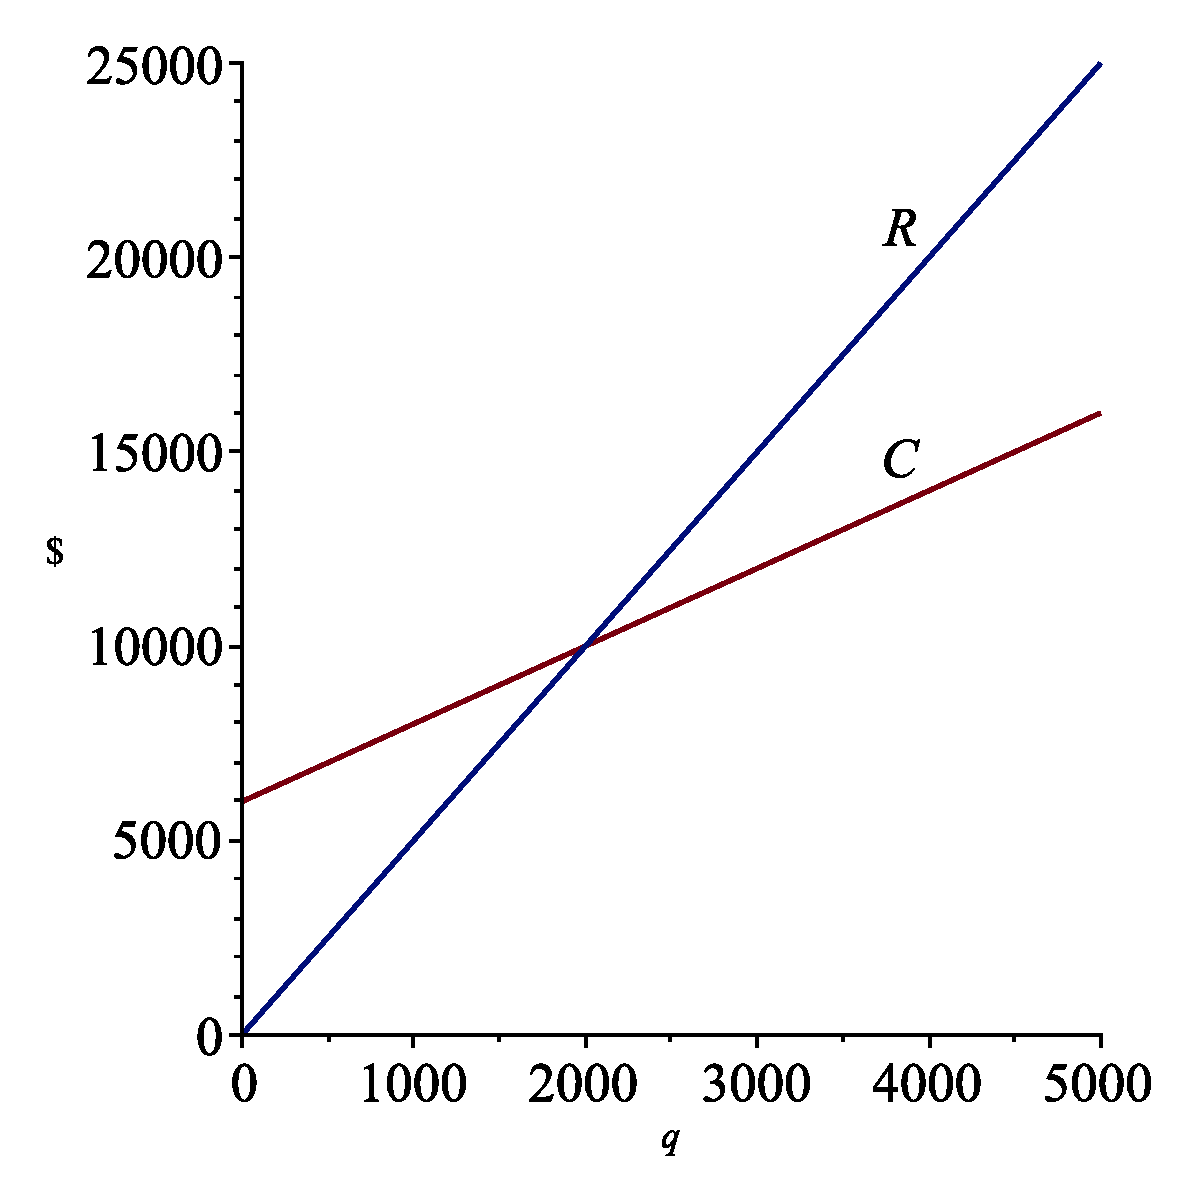
\includegraphics[width=3in]{cost_and_revenue}
\end{center}
It appears from the graph that the break-even point is about
$q=2000$, and this is easy to verify algebraically:
\begin{align*}
C & = R\\
6000 + 2q & = 5q\\
6000 & = 3q\\
q & = 2000\quad  \checkmark
\end{align*}

\item The marginal cost is \$2 per puzzle, the cost of making one
  additional puzzle.  
\end{enumerate}
\end{solution}


\begin{example}[Problem 32]
\small  The demand curve for a product is given by $q=120,000-500p$ and the
  supply curve is given by $q=1000p$ for $0\le q \le 120,000$, where price
  is in dollars.
\begin{enumerate}
\item At a price of \$100, what quantity are consumers
  willing to buy and what quantity are producers willing to supply?
  Will the market push prices up or down?
\item Find the equilibrium price and quantity. Does your answer to
  part (a) support the observation that market forces tend to push
  prices closer to the equilibrium price?
\end{enumerate}
\end{example}

\begin{solution}
\begin{enumerate}
\item 
\begin{align*}
\parbox[b]{1.5in}{quantity consumers are willing to buy}
& = \text{demand}\\
& = 120,000 - 500(100)\\
&  = 70,000\\
\parbox[b]{1.5in}{quantity producers are willing to make}
& = \text{supply}\\
& = 1000(100)\\
& = 100,000
\end{align*}
  At a price of \$100, the supply is larger than the demand, so some
  goods remain unsold and we expect the market to push prices down.

\item
\begin{align*}
\text{equilibrium is where supply} & = \text{demand}\\
120 000 - 500 p & = 1000 p \\
120 000 & = 1500 p\\
p  & = \frac{1200}{15} = \frac{400}{5} = 80 
\end{align*}
The equilibrium price is $\$80$, and the equilibrium quantity is
$ 80,000$.  
  
  The market will push prices downward from \$100, toward the
  equilibrium price of \$80. This agrees with the conclusion to part
  (a) which says that prices will drop.
\end{enumerate}
\end{solution}


\section{Exponential Functions}

\begin{example}[Problem 6]
  The gross domestic product, $G$, of Switzerland was 310 billion
  dollars in 2007. Give a formula for $G$ (in billions of dollars)
  $t$ years after 2007 if $G$ increases by
\begin{enumerate}
\item   3\% per year
\item 8 billion dollars per year
\end{enumerate}
\end{example}

\begin{solution}
  \begin{enumerate}
  \item 
\begin{align*}
G & = P_0 a^t,\ \text{where }a=1+r\\
 a &= 1 + 0.03 = 1.03 \\
& \kern-1em \boxed{G = 310(1.03)^t}
\end{align*}

\item This describes a \emph{constant} rate of change, so it is
  linear.
\begin{align*}
G & = mt+b\\
m &= 8\\
b &= 310\\
&\kern-1em \boxed{G = 8t + 310}
\end{align*}
\end{enumerate}
\end{solution}


\begin{example}[Loyola's Tuition part I]
  For school year 2013--2014, the annual tuition at Loyola University
  Maryland was \$41,850.  For school year 2016--2017, the annual
  tuition at Loyola was \$45,030.   Over this time the
  tuition grew exponentially with an annual percentage rate of growth
  of 2.47\%.
\bigskip

  Assuming that the tuition continues to grow at the same rate, what
  will it be for the 2019--2020 school year?
\end{example}

\begin{solution}
We model the tuition with the following equation
$$
T = 41850 (1.0247)^t
$$
where $t$ is the number of years after 2013.  

For 2019 we  have $t=6$ and so tuition is estimated to be
$$
T = 41850 (1.0247)^6 \approx \$48,448.
$$

% Lisa didn't do this part here.  
% \item Using a graph, predict when the annual tuition will be $\$52,000$.
%   \begin{solution}
%   We want to solve
% $$
% 41850 (1.0247)^t = 52000.
% $$
% We start by graphing $41850(1.0247)^t$ and then find when the
% $y$-value equals $52000$.  
% %Shown below is a plot, with a point marking the $y$-value $52000$.
% %\begin{center}
% %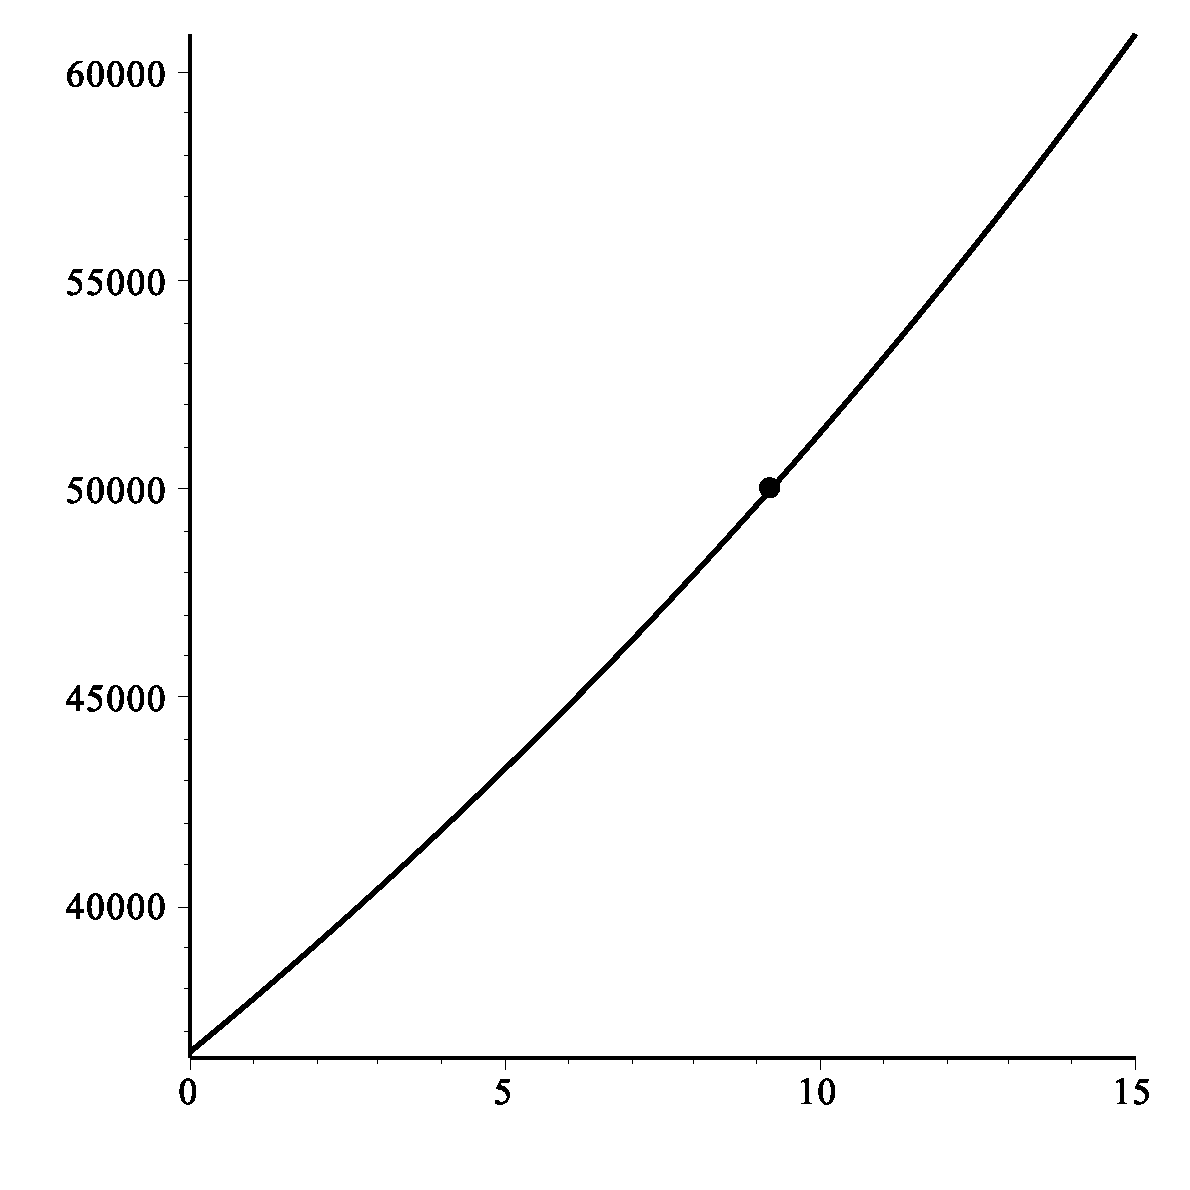
\includegraphics[width=2.5in]{Images/loyola_tuition}
% %\end{center}
% The corresponding $t$-value is approximately $8.9$.  So the tuition
% will be $52000$ in the year corresponding to $t=9$, i.e.\ $2022$.  
\end{solution}


\begin{example}[Loyola's Tuition part II]
  For school year 2013--2014, the annual tuition at Loyola University
  Maryland was \$41,850.  For school year 2016--2017, the annual
  tuition at Loyola was \$45,030.   
\bigskip

  Find $r$, the relative growth rate, so that this growth is modeled
  by an exponential equation.
\end{example}

\begin{solution}
We want tuition to fit into the formula
$$
P = P_0(1+r)^t.
$$
We plug the data into this equation:
\begin{align*}
P_0 & = \text{tuition in 2013}\\
 & = 41850\\
P & = \text{tuition in 2016}\\
 & = 45030\\
t & = \text{the number of years gone by}\\
  & = 3\\
45030 & = 41850 (1+r)^3\\
\frac{45030}{41850} & = (1+r)^3\\
\left(\frac{45030}{41850}\right)^{1/3} & = 1+r\\
r & = \left(\frac{45030}{41850}\right)^{1/3} -1\\
 & \approx 0.02471\\
 & \approx 2.47\%
\end{align*}
\end{solution}


\section{Natural Logarithm}

\begin{example}[Problem 2]
Solve 
$$
10 = 2^t
$$
using natural log.
\end{example}

\begin{solution}
  We can't solve this problem all the way in our heads, but you should
  be able to make a guess that the solution will be between $3$ and
  $4$.  Why? We know $2^3 = 8$ and $2^4 = 16$, so $t$ is somewhere
  between 3 and 4.

Here's how we solve it algebraically:
\begin{align*}
 10 & = 2^t\\
\ln(10) & = \ln(2^t) \\
\ln(10) & = t\ln(2) \\
t & = \frac{\ln(10)}{\ln(2)}\\
 &  \approx 3.3219 
\end{align*}
\end{solution}



\begin{example}[Loyola tuition part III]
In the school year 2013--2014, the annual tuition at Loyola University
Maryland was \$41,850.  Since then it has had an annual growth rate of
$r=2.47\%$.  Assuming this growth rate continues, when will the
tuition reach \$52,000?
\end{example}

\begin{solution}
We plug this data into the model
$$
P = P_0 (1+r)^t
$$  
and solve for $t$:
\begin{align*}
  52000  & = 41850 (1.0247)^t \\
  \frac{52000}{41850} & = 1.0247^t \\
  \ln(52000/41850) & = \ln \left(1.0247^t\right)\\
  \ln(52000/41850) & = t\ln(1.0247)\\
 t  & = \frac{\ln(52000/41850)}{\ln(1.0247)} \\
& \approx 8.8997102
\end{align*}
So, the actual year should be about $2022$.  
\end{solution}


\begin{example}
A city's population starts at 600,000 in 2010 and has a continuous
growth rate of 5\%.  What is the population size in 2017?  
\end{example}

\begin{solution}
We model this city with 
$$
P = 600 000 (1+0.05)^t
$$
and plug in $t=7$:
\begin{align*}
P & \approx 600 000 (1.05)^7\\
  & = 844 260
\end{align*}
\end{solution}


\section{Exponential Growth and Decay}

\begin{example}[Problem 14*]
A population, currently 200, is growing at 5\% per year.
\begin{enumerate}
\item   
Write a formula for the population, $P$, as a function of
time, $t$, years in the future. 

\item   
Graph $P$ against $t$.

\item   
Estimate the population 10 years from now.

\item[(d*)] Find the doubling time of the population algebraically.

\item[(e*)] Model the same population using a continuous
  growth rate, compare the graph of this model with the graph from
  part (b).  
\end{enumerate}
\end{example}

\begin{solution}
\begin{enumerate}
\item $P = 200(1.05)^t$
\item 
\begin{center}
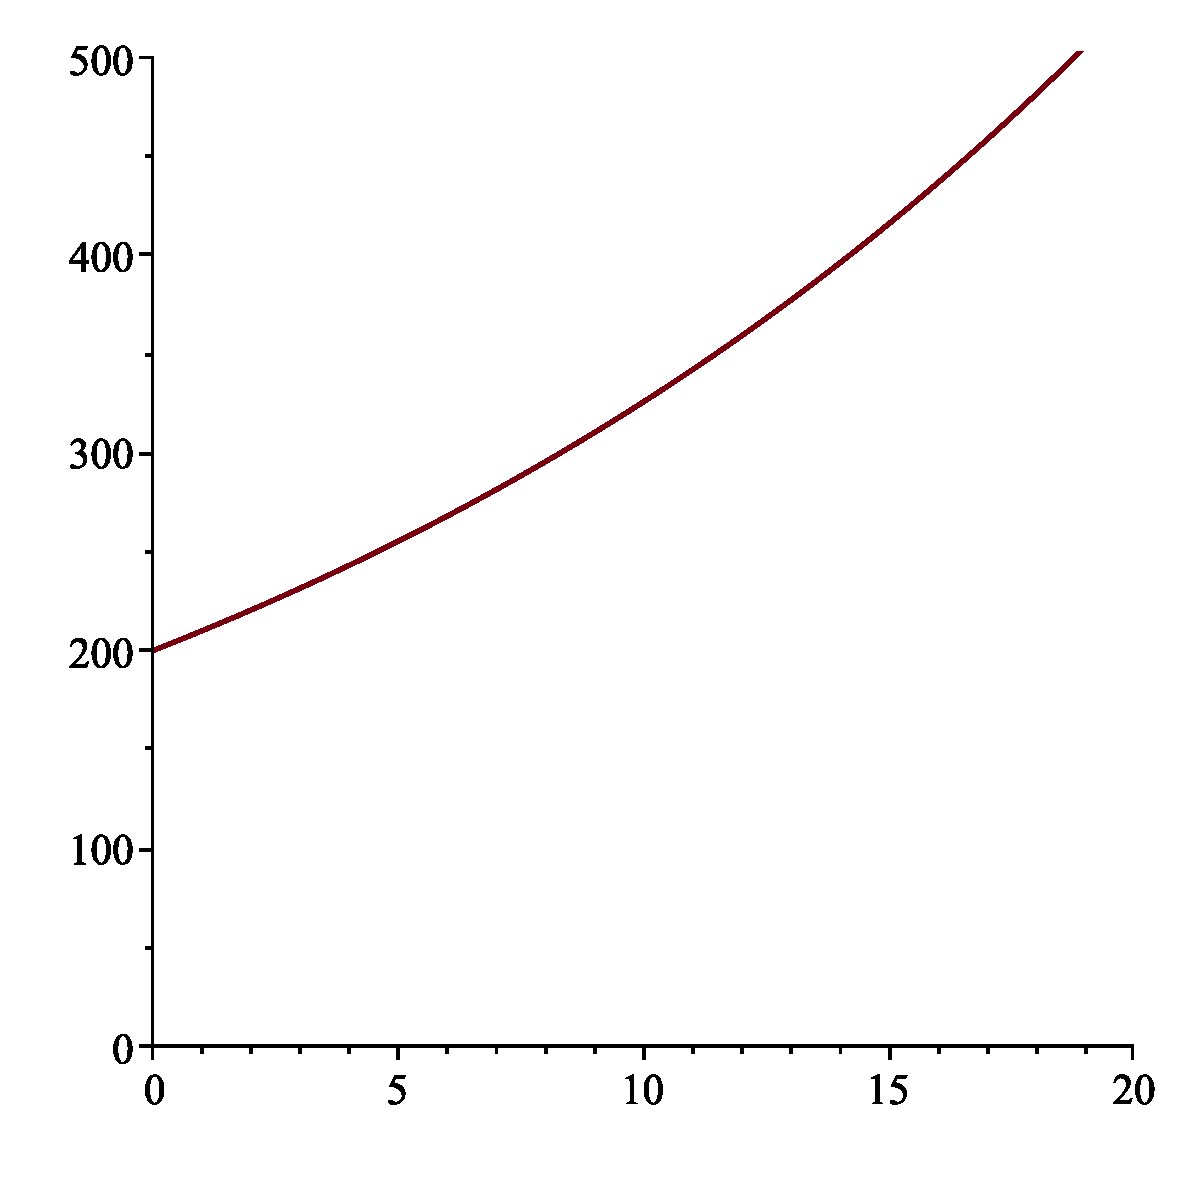
\includegraphics[width=3in]{city_population_growth}
\end{center}

\item \begin{align*}
P(10) & = 200(1.05)^{10}\\
& \approx 325.7789\\
& \boxed{\text{ about }326}
\end{align*}

\item We solve for when $P=400$:
\begin{align*}
 400 & = 200(1.05)^t \\
 2 & = 1.05^t\\
 t & = \ln(2)/\ln(1.05) \\
  & \approx 14.2067 
\end{align*}

\item They are asking to change this model to the natural exponential
  (base $e$, or $Pe^{kt}$ model.  What is the $k$ in this instance?
  \begin{align*}
    200(1.05)^t & = 200e^{kt}\\
    \intertext{We can use $t = 1$(or any value of $t$ but $t=1$ is easiest)}
    1.05 & = e^{k}\\
    \ln(1.05) & = k \ln(e) = k\\
    k & \approx 0.04879
  \end{align*}
  Thus the continuous growth rate is about $4.879\%$ for an annual
  growth rate of 5\%.

  We show below the original function, $P_1$, plotted together with
  the function $P_2 = e^{0.04879t}$, marked with a few little stars,
  $\color{green!75!black}\star$.  As you can see, the original
  function and the new one look identical:
\begin{center}
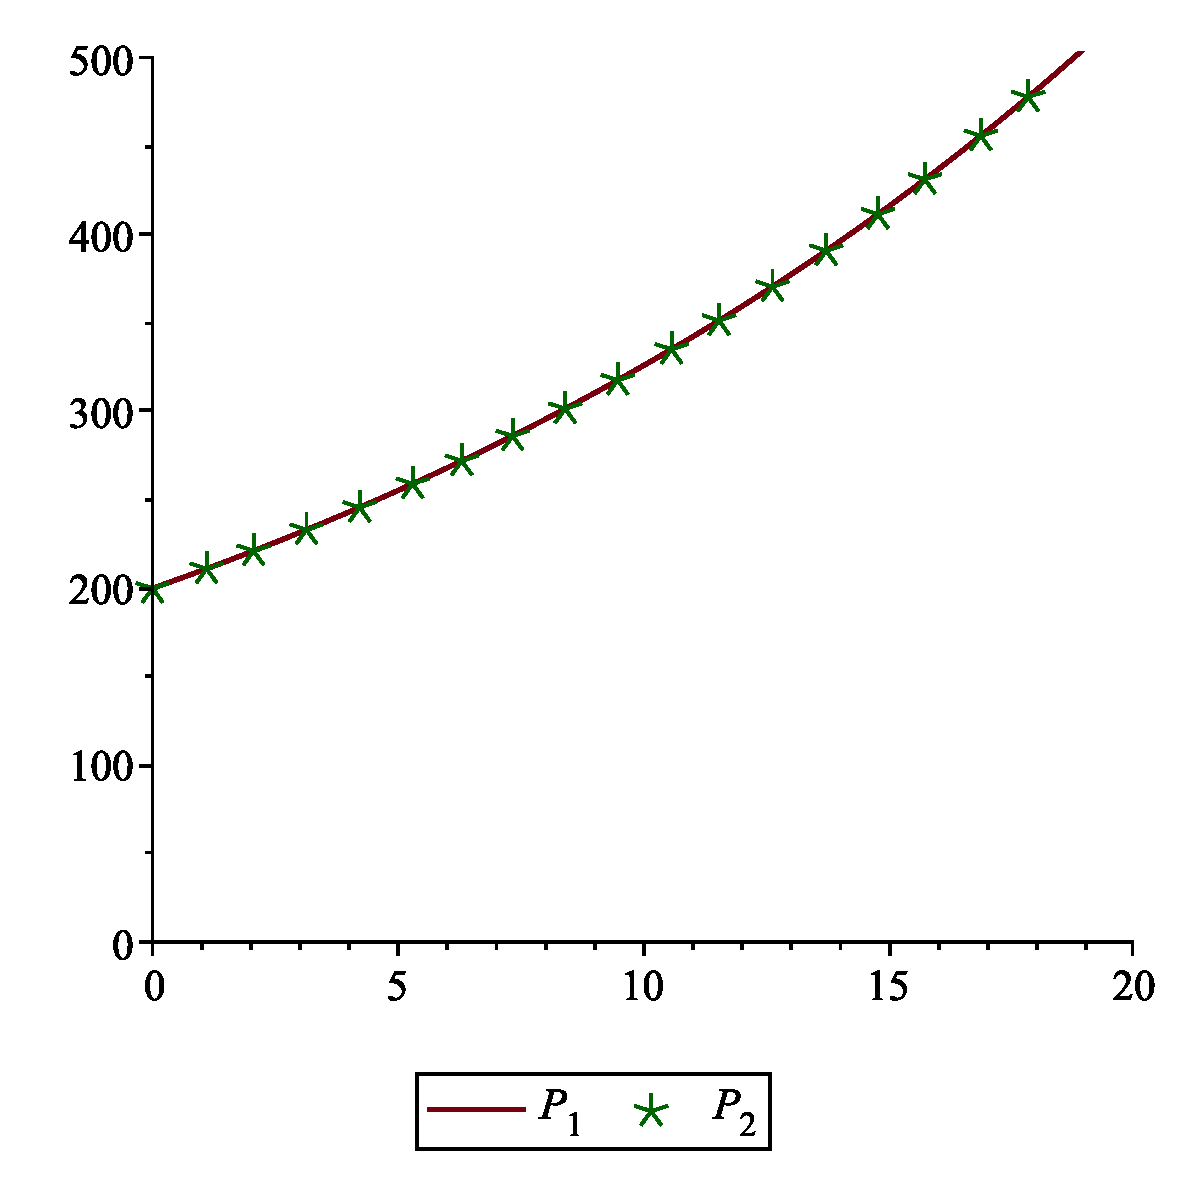
\includegraphics[width=3in]{city_population_two_models}
\end{center}
\end{enumerate}
\end{solution}

\begin{example}
\begin{enumerate}
\item Find the future value in 8 years of a \$7,000 payment today, if
  the interest rate is 3.5\% compounded continuously.

\item Find the present value of a \$7,000 payment that will be made 8
  years from now if the interest rate is 3.5\% compounded
  continuously.
\end{enumerate}
\end{example}

\begin{solution}
\begin{enumerate}
\item We'll use the equation
$$
FV = PV e^{rt}
$$
where $PV = 7000$, $r = 0.035$, and $t = 8$:
$$
 FV = 7000e^{0.035(8)} \approx \$9261.91
$$

\item 
We'll use the equation
$$
FV = PV e^{rt}
$$
where $FV = 7000$, $r = 0.035$, and $t = 8$:
\begin{align*}
 7000 &= PVe^{.035(8)} \\
 PV &= \frac{7000}{e^{.035(8)}}\\
  & = 7000e^{-0.035(8)}\\
  & \approx \$5290.49 
\end{align*}
\end{enumerate}
\end{solution}


\chapter{The Derivative}
\section{Tangent and Velocity Problems}

\begin{example}[Problem 5]
Figure 2.12 shows the cost, $y = f(x)$, of manufacturing $x$ kilograms
of a chemical. 

\begin{center}
 {\large Figure 2.12}\\
  \includegraphics{Images/s2-1prob5.pdf}
\end{center}

\begin{enumerate}
\item Is the average rate of change of the cost greater between
  $x = 0$ and $x = 3$, or between $x = 3$ and $x = 5$? Explain your
  answer graphically.
\item Is the instantaneous rate of change of the cost of producing $x$
  kilograms greater at $x = 1$ or at $x = 4$? Explain your answer
  graphically.
\item What are the units of these rates of change?
\end{enumerate}
\end{example}

\begin{solution}
\begin{enumerate}
\item In the graph below I've marked, by hand, two line segments on
  the curve, i.e.\ two secant lines.  One goes from $x=0$ to $x=3$,
  and the other goes from $x=3$ to $x=5$
\begin{center}
  \includegraphics[width=3in]{Images/s2-1prob5markedA.png}
\end{center}
To compare the average rates of change, you should look at the slope of
each line segment.  Since the one from $x=0$ to $x=3$ is steeper, it
has a greater slope, and therefore the average rate of change is
greater from $x=0$ to $x=3$.


\item In the graph below I've marked, by hand, two tangent lines.  One
  is tangent at $x=1$ and the other is tangent at $x=4$.
\begin{center}
  \includegraphics[width=3in]{Images/s2-1prob5markedB.png}
\end{center}
To compare the instantaneous rates of change, you should look at the
slope of the tangent lines. Since the one at $x=1$ is steeper, it has
a greater slope, and therefore the instantaneous rate of change is
greater at $x=1$.

\item 
The units are, as always,
$$
\frac{\text{units of $y$}}{\text{units of $x$}}
$$
In this case that's
$$
\text{thousands of dollars per kilogram}
$$
\end{enumerate}
\end{solution}

\begin{example}[Problem 12]
Match the points labeled on the curve in Figure 2.14 with the given slopes.
\begin{center}
\renewcommand{\arraystretch}{1.5}
\begin{tabular}{c|c}\hline
Slope &  Point \\ \hline
$-3$  &       \\ \hline
$-1$  &       \\ \hline
$0$   &       \\ \hline
$1/2$ &       \\ \hline
$1$   &       \\ \hline
$2$   &       \\ \hline
\end{tabular}
\bigskip

{\large Figure 2.14}

  \includegraphics[scale=0.75]{Images/s2-1prob12.pdf}
\end{center}
\end{example}

\begin{solution}
We'll justify below the following answers:
$$
\begin{array}{c|c}\hline
\text{Slope} &  \text{Point} \\ \hline
-3  & F     \\ \hline
-1  & C     \\ \hline
0   & E     \\ \hline
1/2 & A     \\ \hline
1   & B     \\ \hline
2   & D     \\ \hline
\end{array}
$$
Let's start by thinking about which point has negative slope: only two
points are marked where the graph is going down: $C$ and $F$.  Which
one is going down more steeply?  You should be able to see that it's
$F$.  So, given the choice of two negative slopes in the table, $-3$
and $-1$, we should choose $F$ to have the slope that's more negative:
$F \to -3$.  Then we must have $C\to -1$.

Now let's think about which point has $0$ slope: this should be where
the tangent line is perfectly horizontal.  There's only one point
where this happens: $E$.  

Finally, let's look at three remaining points, where the slope is
positive.  We can order them by how steep the graph is: It's steepest
at $D$, then next steepest at $B$, and least steep at $A$.  This means
that $D\to 2$, $B\to 1$, and $A\to 1/2$.  
\end{solution}


\begin{example}
Suppose we drop a penny from the roof of a very tall building.  Then
the distance fallen is given by
$$
s(t) = 4.9t^2,
$$
where $s$ is measured in meters, and $t$ is the number of seconds
since the penny has been dropped.  
\begin{enumerate}
\item Find the average velocity from $t=0$ to $t=7$.
\item Estimate the instantaneous velocity at $t=7$.
\end{enumerate}
\end{example}

\begin{solution}
\begin{enumerate}
\item 
\begin{align*}
\text{average velocity} & = \frac{\text{distance traveled}}{\text{time elapsed}} \\
                         & = \frac{s(7) - s(0)} {7-0}                             \\
                       & = \frac{4.9(7^2)-0}{7}                                 \\
                       & = \unitfrac[34.3]{m}{s}
\end{align*}

\item To estimate the instantaneous velocity we find the average velocity over
shorter and shorter time intervals around $t = 7$ seconds.  In other
words, we will calculate this quantity
$$
\frac{s(t) - s(7)} {t-7} = \frac{4.9(t^2)-4.9(7^2)}{t-7}
$$
for values of $t$ that are close to $7$.  

The best way to get a range of values like this is to make a table,
either in your calculator, or in a spreadsheet.  
$$
\begin{array}{c|c}
\text{$t$-value (the one not equal to $7$)} & \text{average velocity from $t$ to $7$} \\
                        & = \frac{s(t)-s(7)}{t-7}                 \\ \hline
6                       & 63.7                                    \\
6.9                     & 68.11                                   \\
6.99                    & 68.551                                  \\
6.999                   & 68.595                                  \\
7.001                   & 68.605                                  \\
7.1                     & 69.09
\end{array}
$$
Once we have this information, we should look just around the rows
that have $t$ as close to $7$ as possible, in this case, those are the
rows with $6.999$ and $7.001$.  In those rows, the velocity is very
close to $68.6$, and so that's our guess:
$$
\text{Instantaneous velocity at $t=7$ is approximately: }
  \unitfrac[68.6]{m}{s}
$$
\end{enumerate}
\end{solution}



\begin{example}
Using a calculator or an equivalent app, estimate $f'(1)$ for $f(x) =
3x^2$.  
\end{example}

\begin{solution}
By definition we have
$$
 f'(1) = \lim_{x \to 1}\frac{f(x) - f(1)}{x-1} .
$$
The way to estimate this is to calculate $\frac{f(x)-f(1)}{x-1}$ for
more than one value of $x$, using values that are close to $1$.  

The best way to get a range of values like this is to make a table,
either in your calculator, or in something like \url{www.desmos.com}:  
$$
\begin{array}{c|c}
\text{$x$-value (the one not equal to $1$)} 
      & \text{average velocity from $x$ to $1$}                            \\
      & = \frac{f(x)-f(1)}{x-1}                                            \\ \hline
  0.5 & 4.500  \qquad \rlap{$\left(=\frac{3(0.5)^2-3(1)^2}{0.5-1}\right)$} \\
0.9   & 5.700                                                              \\
0.99  & 5.970                                                              \\
0.999 & 5.997                                                              \\
1.001 & 6.003                                                              \\
1.01  & 6.030                                                              \\
1.1   & 6.300                                                              \\
1.5   & 7.500 
\end{array}
$$
Once we have this information, we should look just around the rows
that have $x$ as close to $1$ as possible, in this case, those are the
rows with $0.999$ and $1.001$.  In those rows, the difference quotient
is very close to $6$, and so that's our guess:
$$
f'(1) \approx 6
$$
\end{solution}


\begin{example}[Problem 18]
Use Figure 2.16 to fill in the blanks in the following statements
about the function $f$ at point $A$. 
\begin{enumerate}
\item  $f(\blank) = \blank$
\item $f'(\blank) = \blank$
\end{enumerate}
\begin{center}
{\large Figure 2.16}

  \includegraphics[width=3in]{Images/s2-1prob18.pdf}
\end{center}
\end{example}

\begin{solution}
\begin{enumerate}
\item When we write something like ``$f(1)=2$'' we mean that when
  $x=1$ we have $y=2$.  Based on the coordinates of point $A$, we have
  $$
\boxed{f(7) = 3}
$$

\item When we write something like $f'(10) = 11$ we mean that tangent
  line at $x=10$ has slope of $11$.  Based on the graph we can figure
  out $f'(7)$ by calculating the slope of the tangent line.  

  Using the coordinate of the other point on the tangent line, we get
  the slope of the tangent line is
 $$
 m = \frac{3.8 - 3}{7.2-7} = \frac{0.8}{0.2} = 4
$$
so 
$$
\boxed{f'(7) = 4}
$$
\end{enumerate}
\end{solution}

\handoutpagebreak
\section{The Derivative as a Function}
\begin{example}[Problems 18--21]
Match the functions in Problems 18--21 with one of the derivatives in
Figure 2.25.
\begin{center}
\setkeys{Gin}{width=2in}
\renewcommand{\arraystretch}{10}
\begin{tabular}{c@{\hspace{1cm}}c}
\#18\raisebox{-0.75\height}{\includegraphics{s2-2_prob_18}} & \#19\raisebox{-0.75\height}{\includegraphics{s2-2_prob_19}}\\
[15pt]
\#20\raisebox{-0.75\height}{\includegraphics{s2-2_prob_20}} & \#21\raisebox{-0.75\height}{\includegraphics{s2-2_prob_21}}
\end{tabular}
\end{center}
\vfill

\begin{figure}[p]
\centering
{\large Figure 2.25}\bigskip

\setkeys{Gin}{width=2in}
\renewcommand{\arraystretch}{10}
\begin{tabular}{c@{\hspace{1cm}}c}
\includegraphics{s2-2_prob_18-20_I} & \includegraphics{s2_2_prob_18-20_II}\\
\includegraphics{s2-2_prob_18-20_III} & \includegraphics{s2-2_prob_18-20_IV}\\
\includegraphics{s2-2_prob_18-20_V} & \includegraphics{s2-2_prob_18-20_VI}\\
\includegraphics{s2-2_prob_18-20_VII} & \includegraphics{s2-2_prob_18-20_VIII}
\end{tabular}
\end{figure}
\afterpage{\clearpage}
\end{example}

\begin{solution}
Although we have to do all four functions, we don't have to do them
in order.  So, we'll start with the simplest one: \#19.

The function in \#19 is straight line, and it always has the same
slope.  We may not be able to tell exactly what this slope is: maybe
$m=-2$, or $m=-3$ or something like that.  When we look at the graphs
in Figure 2.25 we should not look at their slopes: we should look at
their $y$-values.  Which graph always has a constant $y$-value, of
$y=-2$ or $y=-3$?  Graph IV.  So, \#19 goes with graph IV.

Now let's look at \#20.  Around $x=0$ this has a positive slope: maybe
$m=1$ or $m=2$.  Around $x=2$ this graph is horizontal, so $m=0$.
Around $x=4$ his has a negative slope: maybe $m=-1$ or $m=-2$.  When
we look at the graphs in Figure 2.25 we should not look at their
slopes: we should look at their $y$-values.  Look at $x=0$, and $x=2$
and $x=4$, which graph has $y=-1$ or $y=-2$, then $y=0$, then $y=1$ or
$y=2$?  Graph II.  So, \#20 goes with graph II.

Now let,s look at \#18.  This one is more complicated, but
paradoxically, this means we don't need to be as precise.  There are
two spots where the slope is $0$: at $x=-1$ and $x=1$.  To the far
left the slope is negative; between $x=-1$ and $x=1$ the slope is
positive, and to the far right the slope is negative again.  When we
look at the graphs in Figure 2.25 we should not look at their slopes:
we should look at their $y$-values.  Reading from left to right, we
should look for $y$-values that are negative, $0$, positive, $0$, 
negative, or, to use shorthand:
$$
-, 0, +, 0, -
$$
Which graph has $y$-values that follow this pattern?  Graph VIII.

Finally, let's look at \#21.  See if you can figure out why this
function goes with graph VI.  
\end{solution}

\section{Variations on the derivative}

\begin{example}[Problems 2 and 4]
Write the Leibniz notation for the derivative of the given function
and include units.

\begin{enumerate}
\item[\#2.] The cost, $C$, of a steak, in dollars, is a function of
  the weight, $W$, of the steak, in pounds.

\item[\#4.] An employee's pay, $P$, in dollars, for a week is a
  function of the number of hours worked, $H$.
\end{enumerate}
\end{example}

\begin{solution}
\begin{enumerate}
\item[\#2.]  Since $C$ is a function of $W$, we write $C = f(W)$.  The
  Leibniz notation is $\dfrac{dC}{dW}$ and the units are dollars per
  pound.  

\item[\#4.]  Since $P$ is a function of $H$ we write $P = f(H)$.  The
  Leibniz notation is $\dfrac{dP}{dH}$ and the units are dollars per
  hour.  
\end{enumerate}
\end{solution}

\begin{example}[Problem 6]
  An economist is interested in how the price of a certain item
  affects its sales.  At a price of $\$p$, a quantity, $q$, of the item
  is sold.  If $q = f(p)$, explain the meaning of each of the following
  statements:
  \begin{enumerate}
  \item $f(150) = 2000$
  \item $f'(150) = -25$
  \end{enumerate}
\end{example}

\begin{solution}
\begin{enumerate}
\item In problems like these, the best way to ``explain the meaning''
  is to write a complete, correct, English sentence that uses the
  least amount of technical jargon as possible.  In this case, here
  are some examples:
\begin{center}
``When the price is \$150, there were 2000 items sold.''\\
``If we price it at \$150, then we'll sell 2000 items.''\\
``A price of \$150 leads to sales of 2000.''\\
``We'll sell 2000 items at a price of \$150.''
\end{center}

\item It may help here to practice writing this in Leibniz notation:
$$
\deriv{q}{p}\eval_{p=150}=-25
$$
The reason this notation is useful is that it reminds us that the
derivative is a rate of change, and which units are on top.  Thus,
we can see that the units are ``items per dollar'' and the rate of
change is $-25$.  As before, the best thing to do is to write this
information down in a complete, correct, English sentence:
\begin{center}
\begin{minipage}{3in}
``If the price changes to \$151, we can expect to sell about $25$
fewer items.''
\bigskip

``At the price of \$150, an increase of \$1 will cause the number of
items sold to decrease by \$25.''
\end{minipage}
\end{center}
\end{enumerate}
\end{solution}

\begin{example}
  The cost, $C$ (in dollars), to produce $\ell$ liters of a chemical
  can be expressed as $C = f(\ell)$.  Using units, explain the meaning
  of the following statements in terms of the chemical:
  \begin{enumerate}
  \item $f(350)=1750$

  \item $f'(350)=9$
  \end{enumerate}
\end{example}

\begin{solution}
  \begin{enumerate}
  \item This means that it costs \$1750 to produce 350 liters of chemical.

  \item This means it will cost about \$1759 to produce 351 gallons.
  \end{enumerate}
\end{solution}

\begin{example}
For the function $f(x) = 2\ln(x)$ first
\begin{enumerate}
\item Use a table of numbers to approximate $f'(1)$, and to write the
  equation of the tangent line at the point $(1,0)$.
\item Using linear approximation and your answer to part (a), to
  approximate $f(1.01)$, $f(1.001)$.  
\end{enumerate}
\end{example}



\begin{solution}
\begin{enumerate}
\item Here are some of the values we look at for the difference
  quotient:
$$
\begin{array}{c|c}
\text{2nd $x$-value} & \dfrac{2\ln(x)-2\ln(1)}{x-1}\\ \hline
    0.5000 & 2.7726 \\
    0.9000 & 2.1072 \\
    0.9900 & 2.0101 \\
    0.9990 & 2.0010 \\
    0.9999 & 2.0001 \\
1.0001     & 1.9999 \\
1.0010     & 1.9990 \\
1.0100     & 1.9901 \\
1.1000     & 1.9062 \\
1.5000     & 1.6219
\end{array}
$$
From this table, we estimate that $f'(1) = 2$.  Using this, the tangent line at
\begin{align*}
y & = m(x-x_0) + y_0\\
y & 2(x-1)
\end{align*}

\item The basic idea here is that we can use the tangent line to
  approximate values on the original graph.  Thus
$$
f(1.01) \approx y(1.01) 
$$
where $f(x) = 2\ln(x)$ and $y(x) = 2(x-1)$.  Using this, we have
\begin{align*}
f(1.01) & \approx 2(1.01-1) = 0.02\\
f(1.001) & \approx 2(1.001-1) = 0.002
\end{align*}
(As a way to double check these answers, my calculator says $\ln(1.01)
= 0.009950330$ and $\ln(1.001) = 0.000999500$.  Our estimates are
\emph{very} close to these answers.)

To see why this sort of approximation might be useful, given the
examples we are working with, you have to use your imagination a
little bit.  You need to imagine a function that we \emph{don't} know
much about.  For instance, the exact amount of the total national debt
as a function of, $t$, or the amount of fuel consumption for a truck as
function of its cargo weight, $w$.  In each case, we don't know a
formula for the function.  But we might know what it's current value
is, and how much that value is changing.  Using this, we could
estimate what it's value would be tomorrow, or with a slight increase
in weight.
\end{enumerate}
\end{solution}

\begin{example}[Problem 46]
The area of Brazil's rain forest, $R = f(t)$, in million acres, is a
function of the number of years, $t,$ since 2000.
\begin{enumerate}
\item Interpret $f(9) = 740$ and $f'(9) = -2.7$ in terms of Brazil's
  rain forests.
\item Find and interpret the relative rate of change of $f(t)$ when
  $t = 9$.
\end{enumerate}
\end{example}

\begin{solution}
\begin{enumerate}
\item $f(9) = 740$ tells us that in 2009, the area of Brazil's rain
  forest was 740 million acres.  The formula $f'(9) = -2.7$ tells us
  that in 2009, the area of the rain forest is decreasing by about 2.7
  million acres per year.

\item  
$$
\text{Relative rate of change in 2009} = \frac{f'(9)}{f(9)} =
    \frac{-2.7}{740} \approx -0.00365
$$
Thus in 2009, the rain forests are shrinking at a rate of about
$0.365\%$ per year.
\end{enumerate}
\end{solution}


\begin{example}[Problem 50(b*)]
The world population in billions is predicted to be approximately
$P = 7.1e^{0.011t}$ where $t$ is in years since 2013. Estimate the
relative rate of change of population in 2018 using this model and
$\Delta t = 0.1$.
\end{example}

\begin{solution}
By definition, 
$$
\text{Relative change in 2018} = \frac{P'(5)}{P(5)}
$$
But to use this we first need to find $P'(5)$.  We don't know the
shortcut formula for this yet, so we will estimate it.  Recall  that
$$
P'(5) = \lim_{\Delta t \to 0} \frac{P(5 + \Delta t) - P(5)}{\Delta t}
$$
We use this with $\Delta t=0.1$ to estimate $P'(5)$:
$$
  P'(5) \approx \frac{P(5.1) - P(5)}{0.1} \approx 0.08256
$$
Now we can finish this problem:
$$
\text{Relative rate of change in 2018} \approx \frac{0.08256}{P(5)}
\approx 0.0122858
$$
Another way to put this is that the relative rate of change in $2018$
is approximately $1.2286 \%$ per year.
\end{solution}

\section{The second derivative}

\begin{example}[Problem 2]
  At which of the labeled points, if any, are both $\dfrac{dy}{dx}$
  and $\dfrac{d^2y}{dx^2}$ positive?
  \begin{center}
    \includegraphics[width=2in]{Images/s2-4prob2}
  \end{center}
\end{example}

\begin{solution}
The only point where they are both positive is $B$.  

Here's the proof.  Recall that $\deriv{y}{x}$ is positive when the slope is
positive, and this means the graph is increasing.  The points $B$
and $C$ are the only points where the slope is positive, and so we can
cross off all the other points from our answer: cross off $A$, $D$, and
$E$.

Next, recall that $\frac{d^2y}{dx^2}$ is positive where the graph is
concave up, which means it must have a shape roughly like
\begin{center}
\IncreaseConcaveUp
\quad or \quad
\DecreaseConcaveUp
\end{center}
So, the only points where $\frac{d^2y}{dx^2}$ is positive are at $A$
and $B$.  
\end{solution}


\begin{example}[Problems 4, 6, 8]
Give the signs of the first and second derivatives for the following
functions. Each derivative is either positive everywhere, zero
everywhere, or negative everywhere. 
\begin{center}
\hspace*{-0.5in}
\begin{tabular}{c@{\qquad}c@{\qquad}c}
\#4   \raisebox{-0.75\height}{\includegraphics[width=0.3\textwidth]{Images/s2-4prob4}}
& \#6  \raisebox{-0.75\height}{\includegraphics[width=0.3\textwidth]{Images/s2-4prob6}}
& \#8  \raisebox{-0.75\height}{\includegraphics[width=0.3\textwidth]{Images/s2-4prob8}}
\end{tabular}
\end{center}
\end{example}

\begin{solution}
\begin{enumerate}
\item[\#4] Since this graph is increasing, we have $f'(x)$ is
  positive, which is the same thing as $f'(x)>0$.  Since this graph is
  curving upwards, we have $f''(x)$ is positive.  (Remember: Concave
  up is part of a cup.)
  
\item[\#6] Since this graph is decreasing, we have $f'(x)$ is
  negative, which is the same thing as $f'(x)<0$.  Since this graph is
  not curving at all, we have that $f''(x)$ equals $0$.

\item[\#8] Since this graph is increasing, we have $f'(x)$ is
  positive, which is the same thing as $f'(x)>0$.  Since this graph is
  concave down, we have that $f''(x)<0$.  (Remember: Concave down is
  part of a frown.)
\end{enumerate}
\end{solution}

\begin{example}
  The temperature outside on a given day is given by $f(t){}^\circ C$,
  where $t$ is in hours since midnight.  From 6 AM until noon, the
  first derivative was negative and the second was positive.  Which of
  the following is correct?  You may choose more than one.

  This poll should be done through Poll Everywhere and then discussed
  online.  

  \begin{enumerate}
  \item The temperature was below freezing but getting warmer.
  \item The temperature was below freezing and getting colder.
  \item We do not no whether the temperature was above or below freezing.
  \item The temperature was higher at noon than at 6 AM.
  \item The temperature was lower at noon than at 6 AM.
  \item The temperature was rising but at a slower rate as the morning progressed.
  \item The temperature was rising but at a faster rate as the morning progressed.
  \item The temperature was falling and at a faster rate as the morning progressed.
  \item The temperature was falling but at a slower rate as the morning progressed.
  \end{enumerate}
  \end{example}

\begin{solution}
% (c), (e), and (i).
There is not an ``official'' solution to this, because it is meant to
be a discussion.
\end{solution}

\begin{example}
  Let $P(t)$ represent the price of a share of stock of a corporation
  at time $t$. What does each of the following statements tell us
  about the signs of the first and second derivatives of $P(t)$?
  
\begin{enumerate}
\item ``The price of the stock is falling faster and faster.''
\item ``The price of the stock is getting close to its peak, at which
  it will remain for a little while.'' 
\item ``The price of the stock is skyrocketing.''
\end{enumerate}
\end{example}

\begin{solution} 
  \begin{enumerate}
  \item The phrase ``price \dots is falling'' means $P'(t) < 0$.  Now
    you can draw three kinds of falling graphs:
\begin{center}
\DecreaseStraight
\quad or \quad
\DecreaseConcaveDown
\quad or \quad
\DecreaseConcaveUp
\end{center}
Which of these do you think makes the most sense for ``faster and
faster.'' Probably the middle one.  In that case, it's concave down
(``concave down is part of a frown'') and so  $P''(t) < 0$.

\item For the price to be getting close to its peak, we need that the
  graph is increasing, so $P'(t) > 0$, and starting to level out a
  little bit, so curving like this
\begin{center}
\IncreaseConcaveDown
\end{center}
That means that it's concave down, so $P''(t)<0$.  

\item The price skyrocketing means that it is increasing, so $P'(t) >
  0$.  Also, it's probably not increasing more slowly as time goes on,
  so it's \emph{not} \IncreaseConcaveDown.  Rather, it probably looks like this:
\begin{center}
\IncreaseConcaveUp
\end{center}
This means that it is concave up (``Concave up is part of a cup'') and
so $P''(0)>0$.  
\end{enumerate}
\end{solution}

\section{Marginal Cost and Revenue}

\begin{example}
  It costs \$2500 to produce 1350 items and it costs \$2545 to produce
  1360 items.  What is the approximate marginal cost when producing
  1350 items?
\end{example}

\begin{solution}
We don't have enough information to solve this exactly but we can
approximate it:
\begin{align*}
MC(1350) & = \text{Derivative at }q=1350\\
  & \approx \frac{C(1360)-C(1350)}{1360-1350}\\
  &  = \frac{2545 - 2500}{1360-1350}\\
  &  = \frac{45}{10}\\
  &  = 4.5\\
& \kern-2ex \boxed{MC \approx \$4.50\text{ per item}}
\end{align*}
\end{solution}


\begin{example}[Problem 4*]
Figure 2.55 shows a total cost function, $C(q)$:
  \begin{center}
\includegraphics[width=0.5\textwidth]{Images/s2-5prob4}

{\Large Figure 2.55}
  \end{center}

\begin{enumerate}
\item Estimate the marginal cost when the production level is
  20 and interpret it.

\item Is the marginal cost greater at $q = 5$ or at $q = 30$?
  Explain.

\item Is the marginal cost greater at $q = 20$ or at $q = 40$?
Explain.
\end{enumerate}
\end{example}

\begin{solution}
\begin{enumerate}
\item The best way to do this graphically is to put a ruler on the
  graph at $q=20$ and make it as close to a tangent line as you can.
  Then draw the line and estimate some points on the line.  Maybe you
  get something like this:
\begin{center}
\begin{tikzpicture}
\draw node{\includegraphics[width=2.5in]{Images/s2-5prob4}};
\draw[very thick,red] (-1.5,-0.75) -- ++ (3.3,1); % m = 3.33, but yscale =10
\end{tikzpicture}
\end{center}
It looks like when $q = 20$, we have $C = 200)$ so we have one point
$(20,\ 200)$.  Another point on the tangent line might be
$(50,\ 300)$.  This tangent line would have slope of
$m = \dfrac{300-200}{50-20} = \dfrac{100}{30} = \dfrac{10}{3}$, so
marginal cost would at $q = 20$ is estimated to be about
$10/3 = 3.\overline{3}$.

\item By looking at the tangent lines when $q = 5$ and $q = 30$, both
  would have positive slope but at $q = 5$ the line would be steeper,
  thus the slope would be greater.  Thus marginal cost is greater at
  $q = 5$ than at $q = 30$.

\item By looking at the tangent lines when $q = 20$ and $q = 40$, both
  would have positive slope but at $q = 40$ the line would be steeper,
  thus the slope would be greater.  Thus marginal cost is greater at
  $q = 40$ than at $q = 20$.
\end{enumerate}
\end{solution}


\begin{example}[Problem 8]
Figure 2.57 shows part of the graph of cost and revenue for a car
  manufacturer. Which is greater, marginal cost or marginal revenue,
  at
  \begin{enumerate}
  \item $q_1$?
  \item $q_2$?
  \end{enumerate}
  \begin{center}
    \includegraphics[width=0.5\textwidth]{Images/s2-5prob8}

{\Large Figure 2.57}
  \end{center}
\end{example}

\begin{solution} 
  Remember \emph{not} to look at the gap between the two lines, or at
  which line is higher at which point.  Rather, look at the slopes of
  the two lines, at the points $q_1$ and $q_2$.  Since the graphs are
  lines, the slopes don't change, and we can see that marginal revenue
  is higher for at both points since the slope of the revenue curve is
  greater than the slope of the cost curve at both points.
\end{solution}

\begin{example}
  To produce 2000 items, the total cost is \$4000 and the marginal
  cost is \$15 per item. Estimate the costs of producing:
  \begin{enumerate}
  \item 2001 items
  \item 1999 items
  \item 2050 items
  \end{enumerate}
\end{example}

\begin{solution}
\begin{enumerate}
\item With marginal cost being \$15 when $q = 2000$, this approximates
  the additional cost of producing $2001$ items.  Since it costs
  \$4000 to produce 2000 items, the cost of producing 2001 items is
  estimated to be \$4015.  We can summarize all of this in a linear
  equation:
\begin{align*}
C(2001) & \approx C(2000) + MC(2000) \times \Delta q\\
        & = 4000 + 15 \times 1\\
        & = \boxed{\$4015}
\end{align*}


\item With marginal cost being \$15 when $q = 2000$, this approximates
  the additional cost of producing $2001$ items.  This could also be
  interpreted as the amount of money saved by producing one fewer
  item.  Since it costs \$4000 to produce 2000 items, the cost of
  producing 1999 items is estimated to be
  $\$4000 - \$15 = \$3985$:
\begin{align*}
C(1999) & \approx C(2000) + MC(2000) \times \Delta q\\
        & = 4000 + 15 \times (-1)\\
        & = \boxed{\$3985}
\end{align*}

    
\item With marginal cost being \$15 when $q = 2000$, this approximates
  the additional cost of producing one more item.  Thus to produce 50
  more items, the additional cost is estimated to be $15(50) = 750$.
  Since it costs \$4000 to produce 2000 items, the cost of producing
  2050 items is estimated to be $4000 + 750 = \$4750$:
\begin{align*}
C(2050) & \approx C(2000) + MC(2000) \times \Delta q\\
        & = 4000 + 15 \times 50\\
        & = \boxed{\$4750}
\end{align*}
\end{enumerate}
\end{solution}


\begin{example}[Problem 12]
  Cost and revenue functions for a charter bus company are shown in
  Figure 2.58. Should the company add a 50th bus? How about a 90th?
  Explain your answers using marginal revenue and marginal cost.
  \begin{center}
\includegraphics[width=0.5\textwidth]{Images/s2-5prob12}

{\Large Figure 2.58}
  \end{center}
\end{example}

\begin{solution}
  We need to look at the difference between the marginal costs and
  marginal revenues.  At $q = 50$, the marginal revenue (slope at
  $R(50)$) is greater than the marginal cost (slope at $C(50)$)
\begin{center}
  \begin{tikzpicture}
    \draw node{\includegraphics[width=2.5in]{Images/s2-5prob12}};
    \draw[very thick, red] (-1.5,-1.6) -- ++ (3,1.1) node[right]{$m=C(50)$};
  \end{tikzpicture}
\end{center}
  So the additional revenue of adding the 50th bus will be greater
  than the additional cost.  So yes, it should add a 50th bus.
    
  At $q = 90$, the marginal revenue (slope at $R(90)$) is less than
  the marginal cost (slope at $C(90)$, so no, the 90th bus should not
  be added.
\end{solution}

\chapter{Rules for Derivatives}
\section[Derivatives of power functions]{Shortcuts for powers of $x$,
  constants, sums, and differences}

\begin{example}
Let $f(x)=3x^2-5x+8$.  Find $f'(x)$.  
\end{example}

\begin{solution}
With practice, you can probably just write this down in one step:
$$
f'(x) = 6x -5
$$
But when you are still learning these steps, it might help to break it
down more:
\begin{align*}
f'(x) & = \ddx (3x^2-5x+8) &&\text{``$f'(x)$'' means ``take the derivative''}\\
    &  = \ddx (3x^2) - \ddx(5x) + \ddx(8) && \text{apply the derivative across $+$ and $-$ signs}\\
    &  = 3\cdot 2x^1 - 5\cdot x^0 + 0  && \text{``constant multiple'', ``constant rule'' and ``power rule''}\\
    &  = 6 x  - 5  && \text{just cleaning up}
\end{align*}
\end{solution}

\begin{example}
\begin{enumerate}
\item For $f(x)=6\sqrt{x}$ find $f'(x)$.
\item For $C(q) = q^{13}-\frac{5}{q^3}+7$, find the marginal cost.
\end{enumerate}
\end{example}

\begin{solution}
\begin{enumerate}
\item Before taking the derivative of $\sqrt{x}$ we should rewrite it
  in exponential form, i.e. as a power of $x$:
$$
6\sqrt{x}=6x^{1/2}
$$ 
It's very important that you become comfortable with fractional
exponents: fractional exponents mean you have a root.  

Now we can take the derivative:
\begin{align*}
f' (x) & = \ddx 6\sqrt{x}\\
       & = \ddx 6x^{1/2}\\
       & = 6\cdot \frac 12 x^{\tfrac 12 -1}\\
       & = 3x^{-1/2}\quad \text{or}\quad \frac{3}{\sqrt{x}}
\end{align*}

\item Before taking the derivative of $\frac{5}{q^3}$ we should 
  rewrite it in an exponential form, i.e.\ as a constant times a
  power of $q$:
$$
\frac{5}{q^3} = 5q^{-3}
$$
It's very important that you become comfortable with negative
exponents: negative exponents mean you have ``one over \dots''.

Now we can take the derivative:
\begin{align*}
C'(q) & = \ddq (q^{13}-\frac{5}{q^3}+7)\\
      & = \ddq (q^{13} -5q^{-3}+7)\\
      & = 13q^{13-1} -5(-3)q^{-3-1}+0\\
      & = 13q^{12} +15 q^{-4}\quad \text{or}\quad 13q^{12}+\frac{15}{q^4}
\end{align*}
\end{enumerate}
\end{solution}

\begin{example}
\begin{enumerate}
\item For $y=2.5q^2-0.75q+9.23$, find $y''$.
\item For $C(q) = q(q^2+q^{-2})$, find $C''(q)$.
\end{enumerate}
\end{example}

\begin{solution}
\begin{enumerate}
\item 
\begin{align*}
 y ' & = \ddq (2.5q^2-0.75q+9.23)\\
   & = 2.5(2)q^{2-1}-0.75(1)q^{0}+0&& \text{clean up before taking next derivative}\\
  & = 5q-0.75 \\
y'' & = \ddq (5q-0.75)\\
   & = 5
\end{align*}

\item
In this case we should ``clean up'' \emph{before} you take even the first derivative:
$$
C(q) = q(q^2+q^{-2}) = q^3+q^{-1}
$$
Now we take derivatives:
\begin{align*}
C'(q) & = \ddq (q^3+q^{-1})\\
  & = 3q^2 + (-1) q^{-1-1}\\
  & = 3q^2 - q^{-2}\\
C''(q) & = 3(2)q^{1}-(-2)q^{-2-1}\\
  & = 6q+2q^{-3}
\end{align*}
\end{enumerate}
\end{solution}

\begin{example}
Let $f(x) =3x^2-4x+1$.
\begin{enumerate}
\item Find the equation of the tangent line to $f$ at $(1,0)$

\item Find when $f$ has a horizontal tangent line.
\end{enumerate}
\end{example}

\begin{solution}
\begin{enumerate}
\item We will fill in the following equation
\begin{align*}
y & = m(x-x_0) + y_0\\
x_0 & = 1\\
y_0 & = 0\\
m & = f'(x_0) = f'(1)
\end{align*}
We start by taking the derivative, and then plug this into the equations above:
\begin{align*}
f' (x) & = \ddx (3x^2-4x+1)\\
    & = 6x-4\\
m & = f'(1)\\
  & = 6(1)-4 = 2\\
y & = 2(x-1)+0\\
  & = 2x-2
\end{align*}
Just to double check, you can look at the graphs to see we got it right:
\begin{center}
\includegraphics[width=3in]{"Quadratic and Tangent Line"}
\end{center}

\item First we ``rewrite'' the question, at least in our heads:
\begin{align*}
f \text{ has a horizontal tangent line} & = \text{ means the slope is $0$}\\
  & = \text{ means }f'(x)=0
\end{align*}
Now we set this up as an equation and solve it:
\begin{align*}
f'(x) & = 0\\
6x-4 & = 0\\
6x & = 4\\
x & = 4/6 = 2/3
\end{align*}
Just to double check, you can look at the graphs to see we got it right:
\begin{center}
\includegraphics[width=3in]{"quadratic with horizontal tangent line"}
\end{center}
\end{enumerate}
\end{solution}

\section{Derivatives of exponentials and logarithms}

\begin{example}
Let $f(x) = 3x^3+2e^x$
\begin{enumerate}
\item Find $f'(x)$.

\item Find the equation of the tangent line at $x = 0$.

\item Compare the graph of $f(x)$ and the graph of the tangent line.
\end{enumerate}
\end{example}



\begin{solution} 
\begin{enumerate}
\item Using the constant multiple rule, sum rule, and exponential
  rules:
    $$ 
    f'(x) = 9x^2 + 2e^x 
    $$

\item 
\begin{align*}
 y & = m(x-x_0) + y_0\\
 x_0 & = 0\\
 y_0 & = f(0) = 2\\
 m & = f'(0) = 2\\
y & = 2x+2
\end{align*}

\item We show $f(x)$ and $y=2x+2$ below.  
\begin{center}
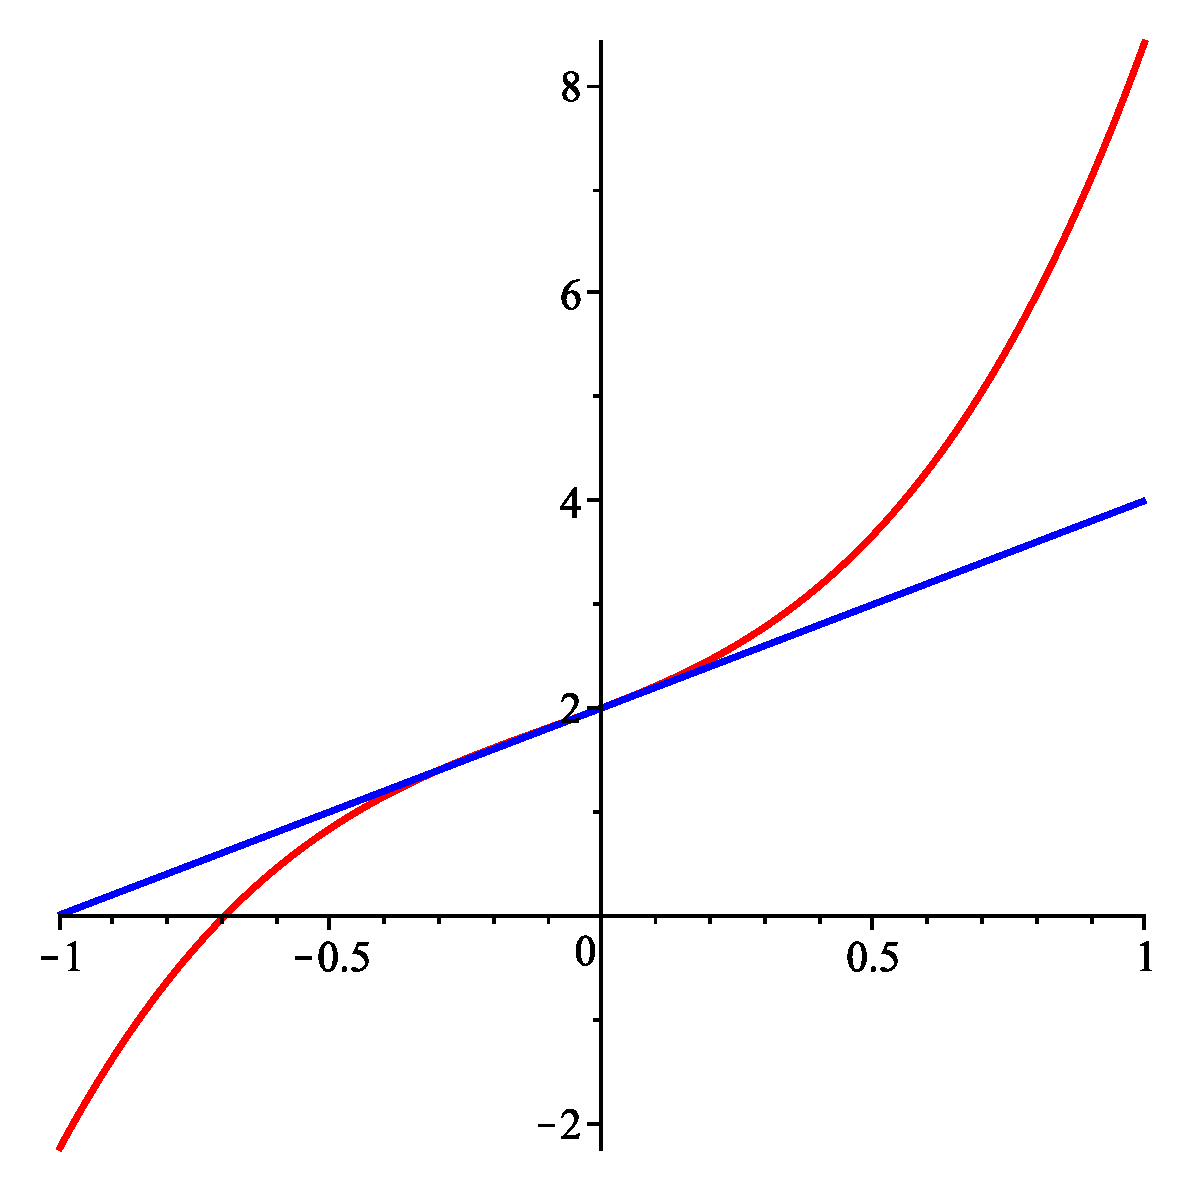
\includegraphics[width=3in]{exponential_with_tangent_line}
\end{center}
\end{enumerate}
\end{solution}



\begin{example}
  The human population of the entire world can be modeled by
  $P = 6.8(1.011)^t$ where $P$ is in billions, and $t$ is the year
  with $t = 0$ corresponding to 2010 (source Wikipedia).
\bigskip



  Find the estimated rate of growth in 2020, and interpret your answer,
  with units.
\end{example}

\begin{solution} 
  Recall that
  $$
  \text{rate of growth} = \text{derivative.}
  $$
Also, the year 2020 means that $t = 10$. Thus, we need to calculate
$P'(10)$, or in Leibniz notation, $\dfrac{dP}{dt}\eval_{t=10}$.
Always find the derivative as a formula first, and then plug in the
number. We use the Constant Multiple Rule and the General Exponential
Rule
\begin{align*} 
  P'(t) &= \ddt (6.8(1.011)t)\\ 
        & = 6.8\BigParens{(1.011)t}'\\ 
        & = 6.8 \ln(1.011)(1.011)^t
\end{align*} 
and plug in $t = 10$:
$$
P'(10) = 6.8 \ln(1.011)(1.011)^{10} \approx 0.083 \text{
      billion people/year}.
$$ 
Here is a simple interpretation:
\begin{quote}
  ``In 2020 the population will increase by 0.083
  billion people each year.''
\end{quote} 
Note: A simpler, and better, statement would convert 0.083 billion to
83 million. I didn't do that above just because I didn't want to
introduce an extra calculation or step into the solution.
\end{solution}

\begin{example}
Find the marginal revenue function if  $R(q) = 4q^2 + 7\ln(q)$.
\end{example}

\begin{solution}
Basically ``marginal revenue'' means we should take the derivative of
$R(q)$.  Really this means we should combine the following basic rules
for derivatives:
\begin{align*}
\ddx \ln(x) & = \frac{1}{x}\\
\ddx c\cdot f(x) & = c\cdot \ddx f(x)
\end{align*}
Now we apply these rules, as well as the power rule from earlier:
\begin{align*}
MR(q) & = R'(q)\\
 & = \ddq \big(4q^2+7\ln(q)\,\big)\\
 & = 4\cdot 2q^1 + 7 \ddq \ln(q)\\
 & = 8q+7\cdot \frac 1q\\
 & =  8q + \frac{7}{q}
\end{align*}
\end{solution}


\section{The Chain Rule}

%%%%%% Section 3.3
% Skipped this in class and videos
% \begin{example}
%   If a car is getting 25 miles per gallon, so it consumes $0.04$
%   gallons per mile and you are driving on cruise control at 60 miles
%   per hour, how many gallons per hour are you consuming?
% 
% 
% \end{example}
% 
% \begin{solution} 
%   If $\dfrac{dG}{dM} = 0.04$ is how many gallons per mile is being
%   consumed by the car, and the speed is $\dfrac{dM}{dH} = 60$ miles
%   per hour, then using the Chain Rule we have
% 
% $$ \dfrac{dG}{dH} = \frac{dG}{dM}\; \frac{dM}{dH} = 0.04(60) = 2.4 \text{ gallons per hour}$$
% \end{solution}
%

%% not sure which to do - did the following in class
\begin{example}
Suppose we are given $A(t) = 1000 e^{0.149t}$.  Find $A'(1)$.
\end{example}

\begin{solution}
  The main idea here is to apply the chain rule to $e^{0.149t}$.  If
  it was just $e^t$ we would use the basic rule, $\ddt e^t = e^t$,
  i.e.\ do nothing.  Since we have $0.149t$ ``inside'' of the
  exponent, we should use the chain rule.  We start with the basic
  rule (do nothing in this case), we don't change the inside, and then
  we multiply by the derivative of the inside.  I'll write this in two
  ways: (1) using an extra variable, $z$, like the book does, to label
  the inside function, (2) using colors and words to keep track of
  what's inside and what's outside.  \emph{You} don't need to write it
  both ways, choose what works best for you.
\begin{gather*}
 % f and g notation, which the book mostly avoids
 % \BigParens{f(0.149t)}' = f'(0.149t)(0.149) \text{ where }f(x) = e^x \\
\begin{aligned}
\ddt e^z & = \deriv{y}{z}\cdot \deriv{z}{t} \text{ where }y=e^z,\text{ and }z=0.149t\\
         & = e^z\cdot (0.149)\\
         & = e^{0.149t}(0.149)
\end{aligned}
\\
% \chain[1]{2}{3}{4}
% #1 = optional shift for target to g(x)
% #2 = lhs of chain rule  
% #3 = f'(\inside{g(x)})           
% #4 = g'(x)              
\text{or} \quad
\raisebox{-0.85\height}{$\chain[(0.5ex,0.5ex)]{\ddt
    e^{0.149t}_{}}{e^{(\inside{0.149t})}_{}}{(0.149)}$}
\end{gather*}
Now we combine this with the rest of the formula for $A(t)$ and
evaluate at $t=1$
\begin{align*}
A'(t) & = 1000 e^{0.149t}(0.149) \\
      & = 149e^{0.149t}          \\
A'(1) & = 149e^{0.149}           \\
      & \approx 172.94
\end{align*}
\end{solution}

\begin{example}
Find the derivatives of 
  \begin{enumerate}
  \item $R = (q^3-5q+7)^5$
  \item $h(x) = \frac{17}{\sqrt{3+5x^2}}$
  \end{enumerate}
\end{example}

\begin{solution}  
  For Chain Rule problems, we want to think of what is the ``outside
  function'' and what is the ``inside function'', and we need each of
  these to be simple enough that we know how to find its derivatives.
  Sometimes it is best to think of the ``outside function'' as the
  last calculation you do.  \bigskip

  For (a), we see that the last calculation that would be done would
  be to take the fifth-power what is in the parentheses.  Thus we'd
  have $z = q^3 -5q+7$ and $R = z^5$.  The Chain Rule gives us
\begin{gather*}
\begin{aligned}
  % R'(q) &= f'(g(q)) g'(q) \text{ where }f(z)=z^5, g(q) = q^3-5q+7 \\
  %       & = 5(g(q))^4 (g'(q)) \text{ where }g'(q) = 3q^2-5\\
  %       & = 5(q^3-5q+7)^4(3q^2-5)\\
\deriv{R}{q} & = \deriv{R}{z} \cdot \deriv{z}{q}, \text{ where }R  = z^5, z= q^3-5q+7\\
        & = 5z^4\cdot (3q^2-5)\\
        & = 5(q^3-5q+7)^4(3q^2-5)
\end{aligned}
\\
% \chain[1]{2}{3}{4}
% #1 = optional shift for target to g(x)
% #2 = lhs of chain rule  
% #3 = f'(\inside{g(x)})           
% #4 = g'(x)              
\text{or} \quad \raisebox{-0.85\height}{\chain{\ddq (q^3-5q+7)^5}
  {5(\inside{q^3-5q+7})^4} {(3q^2-5)}}
\end{gather*}

\bigskip For (b), we need to rewrite the function, changing the
radical in the denominator to a negative exponent:
$h(x) = 17(3+5x^2)^{-1/2}$.  Then we use the Power and Chain Rule
Combined:
$$ 
\chain{\ddx 17(3+5x^2)^{-1/2}} {17\left(-\tfrac{1}{2}\right)(\inside{3+5x^2})^{-3/2}} {(10x)}
$$
We can clean this up, but please be clear in your head: we are done
with the derivative at this point.  The rest is algebra which
\emph{might} be useful, but you also might sometimes not want to do
it, and in any case it's not the new part here.
\begin{align*}
17\left(-\frac{1}{2}\right)(3+5x^2)^{-3/2} (10x)
  & = -\frac{17(10)}{2} (3+5x^2)^{-3/2}x\\
  & = \frac{85x}{(3+5x^2)^{3/2}}
\end{align*}
 \end{solution}

\begin{example}
Find the derivatives of 
\begin{enumerate}    
  \item $y = 5e^{6x} +e^{-x}$
  \item $y = e^{3x^2-7x+11}$
\end{enumerate}
\end{example}

\begin{solution} 
  With exponential functions it's a little tricky to spot what
  ``inside function'' means.  Basically, we should just learn with
  experience that for these, ``inside'' means what's on top.  You can
  make this a little easier to see if you realize that the exponents
  are basically inside implied parentheses:
$$
e^x = e^{(x)},\quad
e^{6x} = e^{(6x)},\quad
e^{-x} = e^{(-x)},\quad
e^{3x^2-7x+11} = e^{(3x^2-7x+11)},\ \text{etc.}
$$
Now ``inside'' really means inside, it's inside the parentheses.  If
you combine this with the Chain Rule you get the following pattern
  \begin{align*}
    y & = e^z,\ z=\text{stuff}
    \deriv{y}{x} & = \deriv{y}{z}\cdot \deriv{z}{x}\\
    y & = e^{\text{(stuff)}} \implies y' = e^{\text{(stuff)}} (\text{stuff})'
  \end{align*}
We'll use this in both parts below.
\bigskip

For (a), we use the Chain Rule on each of the terms, using the pattern
above.  Thus we get
\begin{align*}
  y' & =(5e^{6x}+e^{-x})'\\
     & = 5e^{(6x)}(6x)' + e^{(-x)}(-x)'\\
     & = 5e^{6x}(6)+e^{-x}(-1)\\
     & = 30e^{6x} - e^{-x}
\end{align*}
\bigskip

For (b), we use  the pattern for Exponential Functions and Chain Rule Combined:
\begin{align*}
  y' & = e^{\text{(stuff)}} (\text{stuff})'\\
  y' & =  e^{(3x^2-7x+11)}(3x^2-7x+11)'\\
     & =  e^{(3x^2-7x+11)}(6x-7)\\
     & = (6x-7)e^{3x^2-7x+11}
\end{align*}
Note: it's important that you include the parentheses around $6x-7$:
Without them it's not right, and you will lose points.
\end{solution}

\begin{example}
Find the derivative of $f(x) = \ln(x^2+5)$.
\end{example}

\begin{solution}
Here we have: outside = $\ln(\quad)$ and inside = $x^2+5$.
\begin{gather*}
\begin{aligned}
  \deriv{f}{x} & = \deriv{f}{z} \cdot \deriv{z}{x} \text{ where }z=x^2+5\\
    & = \frac{1}{z}\cdot (2x)\\
    & = \frac{2x}{x^2+5}
\end{aligned}
\\
\text{ or }\raisebox{-0.85\height}{\lnchain{\ddx \ln(x^2+5)}
  {\frac{1}{\inside{x^2+5}}} {(2x)}}
\end{gather*}
This gives us the pattern for natural logarithms with the Chain Rule:
  $$ 
  y = \ln(\text{stuff}) \implies y' = \frac{1}{(\text{stuff})}
  (\text{stuff})' = \frac{(\text{stuff})'}{\text{stuff}}
  $$
\end{solution}

  
% \begin{example}[Problem 36]
% A firm estimates that the total revenue, $R$, received from the sale of $q$ goods is given by
% $$ R = \ln(1 + 1000q^2).$$
% Calculate the marginal revenue when $q = 10$.
% \end{example}
% 
% \begin{solution}
%   We are asked to find $R'(10)$. Using the Log Function and Chain Rule Combined,
%   \begin{align*}
%   R'(q) &= \frac{1}{1+1000q^2}(2000q) = \frac{2000q}{1+1000q^2}\\
%   R'(10) & = \frac{20000}{1+1000(100)} = \frac{20000}{100001} \approx 0.199998
%   \end{align*}
%   So the marginal revenue when producing 10 items is about $0.20$ dollars per unit.
%   \end{solution}


%%%%%% Section 3.4

\section{Product and Quotient Rules}

\begin{example}
Use the Product Rule to differentiate $y = x^2 e^{5x-3}$.
\end{example}

\begin{solution}
  When you are first learning the product rule, you may need to take a
  couple of extra steps to keep the notation straight: (1) Write the
  product rule formula on your paper, right in your solution.  If you
  write this every time, I promise that you'll be able to remember it
  better, and you'll be able to use it better.  (2) Label the parts of
  the function with $f$ and $g$, then find $f'$ and $g'$ and then put
  the parts together where they go in the product rule.
\begin{align*}
(fg)' & = f'\cdot g + f\cdot g'                   \\
f     & = x^2                                     \\
g     & = e^{5x-3}                                \\
f'    & = 2x                                      \\
g'    & = e^{(\text{stuff})}\cdot (\text{stuff})' \\
      & = e^{5x-3}(5)                             \\
y'    & = f'\cdot g + f\cdot g'                   \\
      & = 2x \cdot e^{5x-3} + x^2 \cdot e^{5x-3}(5)
\end{align*}
It's not really necessary to do anything else to this answer: it's not
going to simplify much, and we weren't asked to factor it or anything.
It is traditional to put that last ``5'' in front of the $x^2$, but
it's not mandatory.

Let me show you how you might solve this problem if you've been doing
product rules for a while.  In that case, you might not label $f$ and
$g$ and $f'$ and $g'$.  You might just identify them in your head, and
say the following words to yourself as you go: ``derivative of the
1st, times the second, plus the 1st times the derivative of the
second.''
$$
\underbrace{2x}_{\rotatebox{-90}{deriv. of 1st}}
\underbrace{\cdot \,e^{5x-3}}_{\rotatebox{-90}{times 2nd}} 
+
\underbrace{x^2}_{\rotatebox{-90}{1st}}
\underbrace{\cdot \,e^{5x-3}(5)}_{\rotatebox{-90}{\parbox{0.5in}{times deriv of 2nd}}}
$$
That may seem like a lot to keep track of, or do in your head, but if
you just write and say one part at a time, it's not so bad.  In any
case, do not feel like you should try to do more in your head; feel
free to label everything and arrange all the parts like we did in our
first solution above.  Just know, that if you want to, you can start
to label less as you go.
\end{solution}

\begin{example}
Find the derivatives of the following:
  \begin{enumerate}
  \item $y = x^3(2x-7)^4$
  \item $y = 3t^4 \, \ln(t)$
  \end{enumerate}
\end{example}

\begin{solution} 
Both of these involve the Product Rule.

For (a), the first is $x^3$ and the second is $(2x-7)^4$.  Notice that
finding the derivative of the second will involve the Chain Rule.
  \begin{align*}
  y  & = \big[x^3\big] \ \big[(2x-7)^4\big]                                        \\
  y' & = \big[x^3\big]' \ (2x-7)^4 + x^3\ \big[(2x-7)^4\big]' \\
           & = \big[2x^2\big](2x-7)^4 + x^3\big[4(2x-7)^3(2)\big]                        \\
           & = 2x^2(2x-7)^4 + 8x^3(2x-7)^3
  \end{align*}
  Again, you probably shouldn't try to ``simplify'' any farther here.
  We've taken the derivative, and we're done with that; unless there's
  a reason to factor it, just stop.  \bigskip
  
  For (b), in addition to the Power Rule and Product Rule, we need to
  remember that $\ddt\ln(t) = \frac{1}{t}$.
  \begin{align*}
  y & = \big[3t^4\big]\,\big[\ln(t)\big]\\
  y' & = \big[3t^4\big]'\ln(t) + 3t^4\big[\ln(t)\big]'\\
  & = 12t^3\ln(t) + 3t^4\, \frac{1}{t}\\
  & = 12t^3\ln(t) + 3t^3
  \end{align*}
\end{solution}

\begin{example}
Use the Quotient Rule to differentiate $y = \frac{4t+5}{2-3t^2}$.
\end{example}

\begin{solution} 
  When you are first learning the Quotient Rule, you may need to take
  a couple of extra steps to keep the notation straight: (1) Write the
  Quotient Rule formula on your paper, right in your solution.  If you
  write this every time, I promise that you'll be able to remember it
  better, and you'll be able to use it better.  (2) Label the parts of
  the function with $f$ and $g$, then find $f'$ and $g'$ and then put
  the parts together where they go in the Quotient Rule.
\begin{align*}
\left(\frac{f}{g}\right)' & = \frac{f'\cdot g - f\cdot g'}{(g)^2}\\
f & = 4t+5\\
g & = 2-3t^2\\
f' & = 4\\
g' & = -6t\\
\frac{f'\cdot g - f\cdot g'}{g^2} & = \frac{(4)(2-3t^2)-(4t+5)(-6t)}{(2-3t^2)^2}
\end{align*}
As before, just leave it alone and don't try to simplify, unless
you've been asked to, or if there's a reason to.  In other words,
\textbf{simplify at your own risk}.  (In case you want to practice,
see if you can get $\frac{12t^2+30t + 8}{\left(2-3t^2\right)^2}$\,.)


We can also learn to take the quotient rule without labelling
everything, just like we talked about with the Product Rule.  Here's
how it looks.  Say the following words to yourself as you write things
down: ``derivative of the top, times the bottom, minus the top, times
the derivative of the bottom, all over the bottom squared.''
$$
\frac{
\overbrace{(4)}^{\rotatebox{-90}{deriv top}}
\overbrace{(2-3t^2)}^{\rotatebox{-90}{times bottom}}
-
\overbrace{(4t+5)}^{\rotatebox{-90}{top}}
\overbrace{(-6t)}^{\rotatebox{-90}{times deriv bottom}}
}
{
\underbrace{(2-3t^2)^2}_{\text{bottom squared}}
}
$$
There's a rhyming mnemonic for this as well: ``low d-hi minus hi
d-low, over the bottom squared, and away we go!''.  Here, ``low d-hi''
means derivative of the top (d-hi) times the bottom, etc.
\end{solution}

\begin{example}
Let $f(x) = \frac{e^x}{2x+e^x}$.  
  \begin{enumerate}
  \item Find $f'(x)$.
  \item Find the equation of the tangent line at $x = 0$.
  \end{enumerate}
\end{example}

\begin{solution}
  For part (a), we need to find $f'(x)$ (using the Quotient Rule):
  \begin{align*}
          \left(\frac{f}{g}\right)' & = \frac{f'\cdot g - f\cdot g'}{(g)^2}\\
          f'(x) & = \frac{e^x(2x+e^x) - e^x(2+e^x)}{(2x+e^x)^2}
\end{align*}
Note that we're using $f$ differently in the second line than in the
first one.  That's one reason we have to understand the Product Rule
and Quotient Rule as more than just moving letters around: we need to
understand that in a certain place it's the derivative of the top, not
just the letter $f'$.  \bigskip

For part (b), we'll fill in (as always) the point-slope equation of a line:
\begin{align*}
 y & = m(x-x_0)+y_0\\
 x_0 & = 0 \quad \text{given above}\\
 y_0 & = f(0) \\
     & = \frac{e^0}{0 + e^0} \\
     & = 1\\
m & = f'(0)\\
   & = \frac{e^0(0+e^0) - e^0(2+e^0)}{(0 + e^0)^2}\\
   & = \frac{1(1) - 1(3)}{1^2}\\
   & = -2\\
y & = -2(x-0)+1\\
  & = -2x+1
\end{align*}

They didn't ask us for it, but just for kicks, here's a graph of
$f(x)$ and the tangent line, just to show that we got it right:
\begin{center}
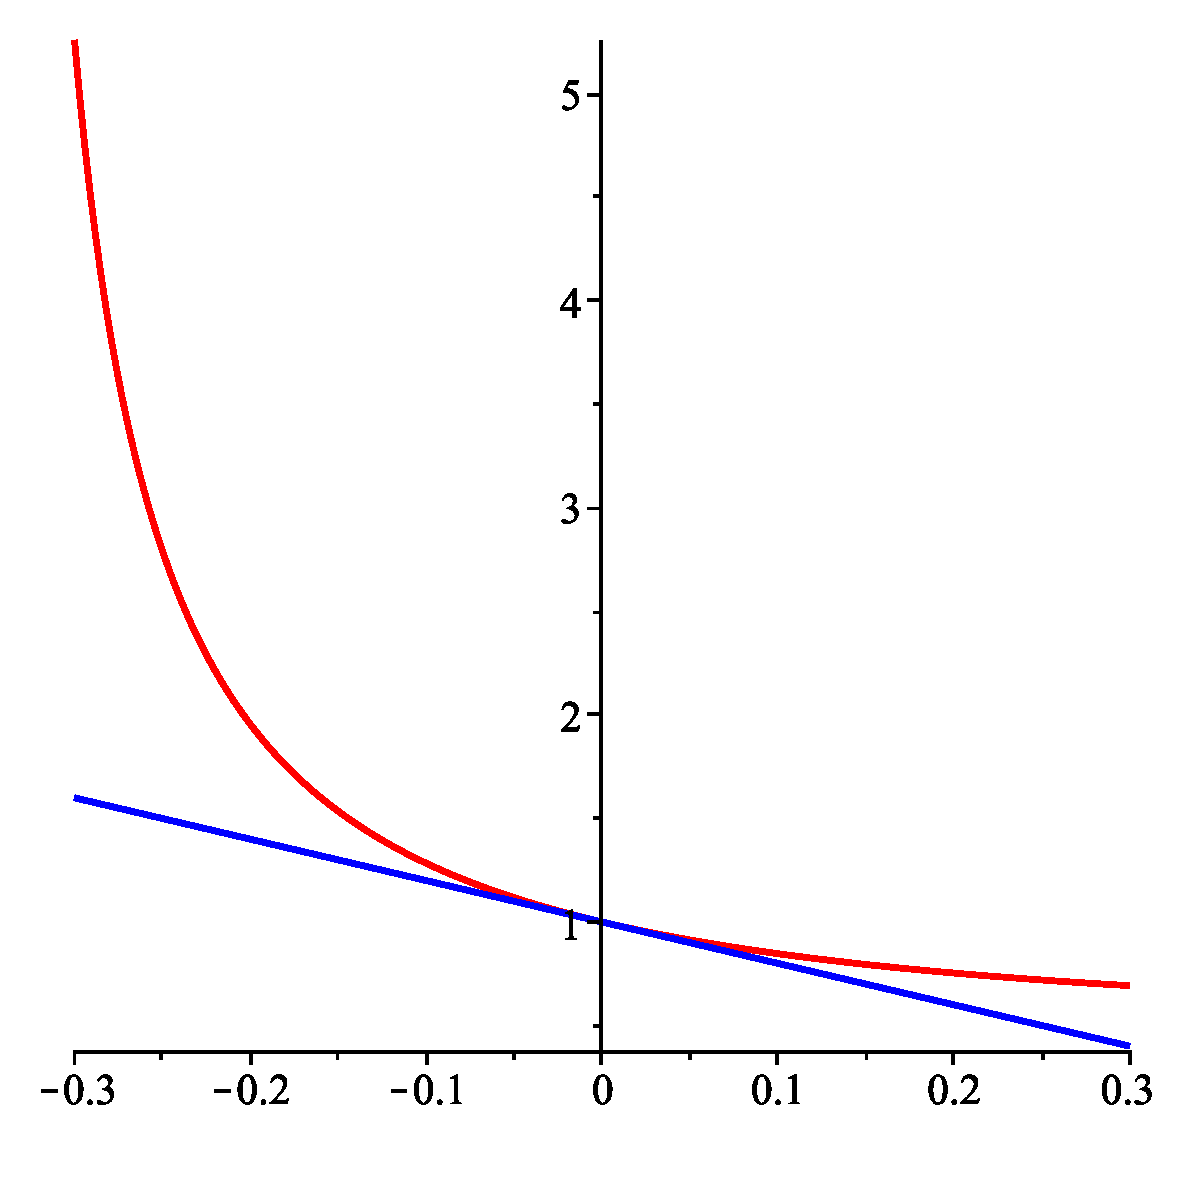
\includegraphics[width=3in]{quotient_rule_with_tangent_line}
\end{center}
\end{solution}



%%%%%% Section 4.1
\chapter{Using the Derivative}
\section{Local Max and Mins}

\begin{definition}
Suppose $c$ is in the domain of $f$:
\begin{itemize}
\item $f$ has a \define{local maximum} at $x=c$ if $f(c) \ge f(x)$ for $x$ near $c$.
  
\item $f$ has a \define{local minimum} at $x=c$ if $f(c) \le f(x)$ for $x$ near $c$.
\end{itemize}
\end{definition}



\begin{definition}
The point $(c,f(c))$ is a \define{critical point} of a function $f$ if either
  \begin{itemize}
  \item $f'(c) = 0$ or
  \item $f'(c)$ is undefined.
  \end{itemize}

The $x$-value, $c$, is a \define{critical number} of $f$.\\
The $y$-value, $f(c)$, is a \define{critical value} of $f$.    
\end{definition}



\begin{example}[Problem 5*]
  \begin{enumerate}
  \item Sketch the graph of a function with two local maxima and one
    local minimum.
  \item Sketch the graph of a function that has two critical points.
    One should be a local maximum and one should be neither a local
    maximum nor local minimum.
  \end{enumerate}
\end{example}

\begin{solution}
There is no ``solution'' for this example: we will discuss it as a group.  
\end{solution}

\begin{test}[First Derivative Test]
  Suppose $c$ is a critical point of a continuous function $f$. When
  moving from left to right:
  \begin{itemize}
  \item If $f'(x)$ changes from positive to negative at $c$, then $f$
    has a \emph{local maximum} at $c$.
  \item If $f'(x)$ changes from negative to positive at $c$, then $f$
    has a \emph{local minimum} at $c$.
  \item If $f'(x)$ does not change sign from at $c$, then $f$ does not
    have a local extremum at $c$.
  \end{itemize}
\end{test}



\begin{test}[Second Derivative Test]
  Suppose $c$ is a critical number for $f$ and $f'(c) = 0$.
  \begin{itemize}
  \item If $f''(c) < 0$, then $f$ has a \emph{local minimum} at $c$.
  \item If $f''(c) > 0$, then $f$ has a \emph{local maximum} at $c$.
  \item If $f''(c) = 0$, then the Second Derivative Test tells us
    nothing.
  \end{itemize}
\end{test}

\begin{example}
  Find all local extrema of the function below, using the Second
  Derivative Test:
$$ 
f(x)= \frac{2}{3}x^3 - 4x^2 - 42x.
$$  
\end{example}

\begin{solution}
Recall the main steps we need for the Second Derivative Test:
\begin{enumerate}
\item Find $f'(x)$
\item Find critical numbers (when $f'(x) = 0$ or $f'(x)$ DNE)
\item Find $f''(x)$.
\item Plug the critical numbers into $f''(x)$ to determine whether the
  critical number(s) are local extrema.
\end{enumerate}

We start by finding $f'(x)$ and setting it equal to $0$:
\begin{align*}
  f'(x) &= 2x^2 - 8x - 42 \\
  2x^2-8x-42 &  =0 \\
  2(x^2-4x-21) & = 0\\
  2(x-7)(x+3)&  =0\\
  x & = 7, -3
\end{align*}
Now we find $f''(x)$ and plug in these critical numbers:
\begin{align*}
  f''(x) & = 4x - 8\\
  f''(7) & = 4(7) - 8 > 0 \implies \text{local min}\\
  f''(-3) & = 4(-3)-8 < 0 \implies \text{local max}
\end{align*}

Finally, we find the critical \emph{points}, i.e.\ the $y$-values that
go along with each critical number.  We do this by plugging the
critical number back into $f$:
\begin{align*}
  f(-3) & = \frac{2}{3}(-3)^3 - 4(-3)^2 - 42(-3) = 72\\
  f(7) & = \cdots = \frac{-784}{3} \approx -261.333
\end{align*}
Thus the function has two critical points: $(-3, 72)$, which is a
local maximum, and $(7,-784/3)$ which is a local minimum.
\end{solution}

\begin{example}
Find and classify all the critical points of the function
$$ 
f(x) = 2x^5(2x-1)^4 + 7. 
$$
\end{example}

\begin{solution}
  We need to find the critical numbers by first finding $f'(x)$.  This
  one involves the Product Rule, and the Chain Rule when we take the
  derivative of the second part (the $(2x-1)^4$).
  $$
  f'(x)  = 10x^4(2x-1)^4 + 2x^5\left(4(2x-1)^3(2)\right)
  $$
  Now we set it equal to $0$ and solve:
  \begin{align*}
    f'(x) & = 0\\
    10x^4(2x-1)^4 + 16x^5(2x-1)^3& = 0
  \end{align*}
  Note the common factors of $2$, $x^4$, and $(2x-1)^3$:
  \begin{align*}
    2x^4(2x-1)^3 \BigParens{5(2x-1) + 8x} & = 0\\
    2x^4(2x-1)^3 \BigParens{10x-5+8x} & = 0\\
    2x^4(2x-1)^3(18x-5)& = 0\\
    2x^4 & = 0\text{ or }(2x-1)^3 =0 \text{ or }(18x-5) = 0\\
    x & = 0, 1/2, 5/18
  \end{align*}
  
  It would take a lot of work (multiple Product Rules) to
  find $f''(x)$ to use the Second Derivative Test.  Thus the First
  Derivative Test might be better in this case. So we want to find
  when $f'(x)$ is negative and positive, and when the derivative
  changes sign to find the local extrema (if any).
  
  So we look at $f'(x) = 2x^4(2x-1)^3(18x-5)$ and we see that the only
  time $f'(x)$ changes sign is when it equals zero, which are the
  critical numbers: $x = 0$, $5/18$, and $1/2$. Note that
  $5/18 \approx 0.277778$.
  
  To organize my work, I draw a number line with the critical numbers
  marked.  Then I calculate $f'(x)$ on each side of each critical
  number.  Note that I don't calculate the actual value, just whether
  the derivative is positive or negative.  This makes things
  \emph{much} faster.  For example, we are looking at
  $f'(x) = 2x^4(2x-1)^3(18x-5)$ and wondering whether $f'(x)$ is
  positive or negative to the left of $0$ (for $x < 0$).  So I choose
  one value, say $x = -1$, and plug it into $f'(x)$.  Since it is
  factored, I look at whether each factor is positive or negative,
  keeping in mind whether the powers are odd or even.  So for $f'(-1)$
  I get: $2(+)(-)(-) = (+)$, and mark this on the number line.  We
  could have chosen a different value to plug in, like $x=-2$, or
  $x=-1/2$, or $x=-10$ and the net result would have been the same.
  We need to pick three more values in the other parts of the number
  line.  Here are an easy three to use: $x=4/18$, $x=6/18$, and $x=1$
  (I used something over $18$ to make the factor $(18x-5)$ easy to
  figure out).  Here's the finished result
  \begin{center}
    \begin{tikzpicture}[scale = 1.25]
      % \draw[step=1cm,gray,ultra thin] (-2.2,-3.2) grid (7.2,5.2);
      \draw[<->] (-4,0) -- (4,0);
      \foreach \x/\l in {-2/0, 0/{5/18}, 2/{1/2}}
      \draw (\x,0.4) -- (\x,-0.6) node[below]{\large $\l$};
      
      \draw (0,0.5) node[above] {\small $f'(x) = 2x^4(2x-1)^3(18x-5)$};
      \draw (-4,0) node[above] {\small $2(+)(-)(-) = (+)$};
      \draw (-4,0) node[below] {\small $f'(x) > 0$};
      \draw(-4,-1) node {\small $f \nearrow$};
      
      \draw (-1,0) node[above] {\small $2(+)(-)(-)$};
      \draw (-1,0) node[below] {\small $f'(x) > 0$};
      \draw(-1,-1) node {\small $f \nearrow$};
      
      \draw (1,0) node[above] {\small $2(+)(-)(+)$};
      \draw (1,0) node[below] {\small $f'(x) < 0$};
      \draw(1,-1) node {\small $f \searrow$};
      
      \draw (3,0) node[above] {\small $2(+)(+)(+)$};
      \draw (3,0) node[below] {\small $f'(x) > 0$};
      \draw(3,-1) node {\small $f \nearrow$};
    \end{tikzpicture}
\end{center}

From the above information and the First Derivative Test, we see that
there is a local maximum at $x = 5/18$, and a local minimum at
$x = 1/2$, and the critical point at $x = 0$ is not a local extremum.
But they asked for critical \text{points}, so we have to figure out
the $y$-values of these points.  Go all the way back to the original
function $f(x)=2x^5(2x-1)^4$ (not $f'$!) and plug in the critical
numbers:
  \begin{align*}
    f(x) &= 2x^5(2x-1)^4 + 7\\
    f(0) &= 7\\
    f(5/18) & = 2\left(\tfrac{5}{18}\right)^5 \BigParens{2\left(\tfrac{5}{18}\right) - 1}^4 + 7\\
         & = 2\frac{5^5}{18^5}\left(-\frac{4}{9}\right)^4 + 7 \\
         & = \frac{3125(256)}{944784(6561)} + 7\\
         & \approx 7.000129\\
    f(1/2) & = 2\left(\tfrac{1}{2}\right)^5\BigParens{2(\tfrac{1}{2}) - 1}^4 + 7 \\
         & = \frac{1}{16}(0) + 7 =  7\\
  \end{align*}
Finally, we can summarize our answer
\begin{align*}
  (0, 7): & \text{ not a local extremum}\\
  (5/18, 7.000129):& \text{ local maximum}\\
  (1/2, 7):& \; \text{ local minimum}
\end{align*}
\end{solution}
  
%%%%%% Section 4.2
\section{Inflection points}

\begin{definition}
An \define{inflection point} for a function $f(x)$ is a point on the
graph of $f(x)$ where the concavity changes.  \bigskip

An inflection point is where $f''(x)$ changes from positive to
negative, or from negative to positive.
\end{definition}

\begin{example}
Find all critical points and inflection points of the function
$$ 
f(x) = x^3 - 12x + 8.
$$
Identify each critical point as a local max, local min, or neither.  
\end{example}

\begin{solution}
We start by taking the derivative and setting it equal to $0$:
\begin{align*}
f' (x) & = 3x^2-12\\
3x^2-12 & = 0\\
3(x^2-4) & = 0\\
3(x+2)(x-2) & = 0\\
x= -2, 2
\end{align*}
Our critical numbers are $-2$ and $2$.  We'll test these with the
second derivative test:
\begin{align*}
f''(x) & = 6x\\
f''(-2) & = -12 \Rightarrow f'' \text{ is }-, f\text{ is C.D., graph is \GenericConcaveDown}\\
f''(2) & = 12 \Rightarrow f'' \text{ is }+, f\text{ is C.U., graph is \GenericConcaveUp}
\end{align*}
Therefore we can identify the behavior at each critical number
\begin{align*}
x & = -2 \text{ local max}\\
x & = 2 \text{ local min}
\end{align*}
Now we find the inflection points. We start by setting the second
derivative equal to $0$:
\begin{align*}
f''(x) & = 0\\
6x & = 0\\
x & = 6
\end{align*}
It's easy to see that $f''(x) = 6x$ is negative to the left of $x=0$
(just plug any negative number into $6x$) and it's positive to the
right of $x=0$.  Thus, $x=0$ is the location of an inflection point.

Finally, we calculate the $y$-values at the critical points and the
inflection point.  We do this by plugging back into the original $f$
(not $f'$ or $f''$!).
\begin{align*}
f(x) & = x^3-12x+8\\
f(-2) & = 24\\
f(0) & = 8\\
f(2) & = -8
\end{align*}
\end{solution}

\begin{example}
Find all inflection points of each of the functions below
% Identify each critical point as a local max, local min, or neither.  Graph it.
$$ 
f(x)  = x^9 \quad\text{and}\quad g(x) = x^6
$$
\end{example}

\begin{solution}
  We start by finding where the second derivative of each of these is
  $0$, and then look at whether the second derivative is positive or
  negative on either side of these numbers.

\begin{align*}
f'(x) & = 9x^8\\
f''(x) & = 72x^7\\
72 x^7 & = 0\\
x& = 0
\end{align*}
Now we look to the left and the right of $0$.  For instance, is
$f''(x)$ positive or negative when we look at $x=-1$?
\begin{align*}
f''(-1) & = - \Rightarrow f \text{ is C.D.}\\
f''(1) & = + \Rightarrow f \text{ is C.U.}
\end{align*}
In other words, $f$ changes from C.D. to C.U. at $x=0$, so $x=0$ is
the location of an inflection point.

\begin{align*}
g'(x) & = 6x^5\\
g''(x) & = 30x^4\\
30 x^4 & = 0\\
x& = 0
\end{align*}
Now we look to the left and the right of $0$.  For instance, is
$g''(x)$ positive or negative when we look at $x=-1$?
\begin{align*}
g''(-1) & = + \Rightarrow g \text{ is C.U.}\\
g''(1) & = + \Rightarrow g \text{ is C.U.}
\end{align*}
In other words, $g$ does \emph{not} change concavity at $x=0$, so
$x=0$ is not the location of an inflection point.
\end{solution}


% \begin{example}
% Find all  inflection points of the function  %Identify each critical point as a local max, local min, or neither.  Graph it.
%   $$ 
%         f(x)  = 5x^3 - 3x^5.
%         $$
% \end{example}
% 
% \begin{solution}
% 
% \end{solution}

\begin{example}[Problem \#26]
  Sketch a possible graph of $y = f(x)$, using the given information
  about the derivatives $y' = f'(x)$ and $y'' = f''(x)$.  (Assume that
  the function is defined and continuous for all real $x$.)
\begin{center}
\begin{tikzpicture}
  \matrix (DerivGrid) [matrix of math nodes,row sep = 5pt]
{
% 1 & 2       & 3       & 4     & 5     & 6 & 7      & 8    & 9  \\
    &         & y' = 0  & {}    &       &   & y' = 0 &      &    \\
    & y'>0    &         &       & y'>0  &   &        & y'<0 &    \\
{}  &         &         &       &       &   &        &      & {} \\
    &         & x_1     &       & x_2   &   & x_3    &      &    \\
    &         & y'' = 0 &       & y''=0 &   &        &      &    \\
    & y'' < 0 &         & y''>0 &       &   & y''<0  &      &    \\
{}  &         & {}      &       & {}    &   & {}     &      & {} \\
};
\begin{scope}[<->,thick]
\draw (DerivGrid-3-1.west) -- (DerivGrid-3-9.east);
\draw (DerivGrid-7-1.west) -- (DerivGrid-7-9.east);
\end{scope}
\begin{scope}[densely dotted]
\draw (DerivGrid-1-3.south) -- (DerivGrid-4-3.north) 
      (DerivGrid-4-3.south) -- (DerivGrid-5-3.north)
      (DerivGrid-5-3.south) -- (DerivGrid-7-3.south);
\draw (DerivGrid-2-5.south) -- (DerivGrid-4-5.north) 
      (DerivGrid-4-5.south) -- (DerivGrid-5-5.north)
      (DerivGrid-5-5.south) -- (DerivGrid-7-5.south);
\draw (DerivGrid-1-7.south) -- (DerivGrid-4-7.north) 
      (DerivGrid-4-7.south) -- (DerivGrid-6-7.north)
      (DerivGrid-6-7.south) -- (DerivGrid-7-7.south);
\end{scope}
\end{tikzpicture}
\end{center}
\end{example}

\begin{solution}
  From the information in the chart, we see that $y'=0$ at $x_1$ and
  $x_3$.  This means that $x_1$ and $x_3$ are critical numbers.

  Can we say if these points are local max or mins?  Yes.  We have
  that $y'$ is positive on both sides of $x_1$, and $y'$ changes from
  positive to negative at $x_3$.  We can summarize this info in a
  picture
\begin{center}
\begin{tikzpicture}
% Let x_1,x_2 and x_3 be at 1, 2, 3
\draw (-0.5,0) -- (3.5,0);
\foreach \x in {1,3} \xtickmark[x_\x]{\x};
\draw (0,0) node[above]{$f:$};
\draw (0.5,0) node[above]{$\nearrow$};
\draw (1.5,0) node[above]{$\nearrow$};
\draw (3.5,0) node[above]{$\searrow$};
\end{tikzpicture}
\end{center}
This makes it easy to see that $x_1$ is neither a max nor a min, but,
on the other hand, $x_3$ is a local max.

From the information in the chart, we see that $y''=0$ at $x_1$ and
$x_2$.  This means that $x_1$ and $x_3$ are possible locations of
inflection points.

Can we say if inflection points really occur here?  Yes.  We have that
$y''$ changes from negative to positive at $x_1$, and changes back to
negative again at $x_2$.  We can summarize this info in a picture
\begin{center}
\begin{tikzpicture}
% Let x_1,x_2 and x_3 be at 1, 2, 3
\draw (-0.5,0) -- (3.5,0);
\foreach \x in {1,2} \xtickmark[x_\x]{\x};
\draw (0,0) node[above]{$f:\qquad$};
\draw (0.5,0) node[above]{C.D.};
\draw (1.5,0) node[above]{C.U.};
\draw (2.5,0) node[above]{C.D.};
\end{tikzpicture}
\end{center}
This makes it easy to see that $x_1$ and $x_2$ are both locations of
inflection points.  Here's a sketch of the shape that $f$ must have (I
only claim this is the shape: the $y$-values could be positive or
negative, the whole picture could be stretched in one direction, or
compressed, etc.)
\begin{center}
\begin{tikzpicture}
\draw (0,0) parabola bend (1,1) (1,1) 
parabola (2,2)
parabola bend (3,3) (3,3) 
parabola (4,2);
\begin{scope}[dashed]
\draw (1,1) -- (1,0) node[below]{$x_1$};
\draw (2,2) -- (2,0) node[below]{$x_2$};
\draw (3,3) -- (3,0) node[below]{$x_3$};
\end{scope}
\end{tikzpicture}
\end{center}
\end{solution}

\begin{example}
Graph a function with the given properties.
\begin{enumerate}
\item Has local minimum and global minimum at $x = 3$ but no local or
  global maximum.
\item Has local minimum at $x = 3$, local maximum at $x = 8$, but no
  global maximum or minimum.
\item Has no local or global maxima or minima.
\item Has local and global minimum at $x = 3$, local and global
  maximum at $x = 8$.
\end{enumerate}
\end{example}

\begin{solution}
Discussion opportunity.
\end{solution}

% Section 4.3

\section{Global max and min}

\begin{test}[Global Max/Min Test]
To find the global max and global min of $f(x)$ on an interval:
\begin{enumerate}
\item Find the critical numbers

\item Compare the values for $f(x)$ at the critical numbers and at the
  ends of the interval.
\end{enumerate}
\bigskip

``Values for $f(x)$'' means you plug the critical numbers and ends of
the interval into $f(x)$ and calculate the result.
\end{test}



\begin{example}
  For the function
  $$ 
  f(x) = x^5 - 2x^4, \quad -1 \le x \le 2
  $$
  identify any global maxima and minima of $f$ in the given interval.
\end{example}

\begin{solution}
  We start, as always, by finding the critical numbers.  In other
  words, we take the derivative and set it equal to $0$.

  For $f(x) = f(x) = x^5 - 2x^4$,
  \begin{align*}
    f'(x)     & = 5x^4-8x^3 \\
    5x^4-8x^3 & = 0         \\
    x^3(5x-8) & = 0         \\
    x         & = 0,\quad x = \frac{8}{5}
  \end{align*}
  Now it's rather easy to finish: we plug these critical numbers back
  into $f$ (not $f'$!), and do the same thing with the end points,
  $x=-1$ and $x=2$, and simply look at which produces the largest
  $y$-value and which produces the smallest $y$-value:
  \begin{align*}
    f(0) & = 0, \\
    f(8/5) &= (8/5)^5 - 2(8/5)^4\\
         & =  \frac{32768}{3125} - \frac{2(4096)}{625} \\
         & = \frac{-8192}{3125} \\
         & \approx -2.62144\\
    f(-1) & = -1-2\\
         & = -3\\
    f(2) & = 32 - 32\\
         & = 0
  \end{align*}
  Now, simply look at the $y$-values: $0$, $-2.62$, $-3$ and $0$
  again, and identify the largest and smallest.

We can summarize our findings:
\begin{align*}
(0,0) \text{ and }(2,0) :& \quad\text{Global Max}\\
(-3, -2.62): & \quad\text{Global Min}
\end{align*}
\end{solution}


%\begin{example}
% The product of two positive numbers is 1936. What is the minimum value of their sum?
%\end{example}
%
%  \begin{solution}
%  $xy = 1936 \implies y = \dfrac{1936}{x}$.\\
%  We want to find the minimum of $x + y = x + \frac{1936}{x}$. Also we need $x > 0$ since we need both numbers to be positive.
%  \begin{align*}
%  S(x) & = x + \frac{1936}{x} = x + 1936x^{-1}\\
%  S'(x) & = 1 - 1936x^{-2} = 1 - \frac{1936}{x^2}\\
%  & = \frac{x^2-1936}{x^2}
%  \end{align*}
%  We see there are critical numbers when $x = \pm \sqrt{1936} = \pm 44$ but we only care about $x = 44$.  Look at  $S''(x) = 1936x^3$ we see that $S''(44) > 0$ so by the Second Derivative Test, $X = 44$ gives us a minimum sum.  The minimum sum is
%  $$ S(44) = 44 + \frac{1936}{44} = 44 + 44 = \boxed{88}.$$
%  \end{solution}


\begin{example}
  The energy expended by a bird per day, $E$, depends on the time
  spent foraging for food per day, $F$ hours. Foraging for a shorter
  time requires better territory, which then requires more energy for
  its defense. Find the foraging time that minimizes energy
  expenditure if
  $$ 
  E = 0.25F + \frac{1.7}{F^2}
  $$
\end{example}

\begin{solution}
  To find the minimum value of $E$, we do what we always do: take the derivative and set it equal to $0$:
  \begin{align*}
    \deriv{E}{F}              & = 0.25 - \frac{2(1.7)}{F^3}           \\
    0.25 - \frac{3.4}{F^3} & = 0                                   \\
    F^3                    & = \frac{2(1.7)}{0.25}                 \\
    F                      & = \left(\frac{3.4}{0.25}\right)^{1/3} \\
                           & \approx 2.3870
  \end{align*}
  Looking at the second derivative, we see it is always positive, so a
  foraging time of $F \approx 2.387$ hours gives a local minimum.
  This is the global minimum for $F > 0$ (graph it to verify).
\end{solution}

\section{Optimizing Cost and Revenue}

\begin{discussion}
  Suppose you're looking at a demand curve.  What does the point on
  the curve where $p=0$ mean?  What does the point where $q=0$ mean?
\end{discussion}


\begin{example}
  Let $C(q)$ be the total cost of producing a quantity $q$ of a
  certain product. See Figure below (Figure 4.52 in the text).
  \begin{enumerate}
  \item What is the meaning of $C(0)$?
  \item Describe in words how the marginal cost changes as the
    quantity produced increases.
  \item Explain the concavity of the graph (in terms of economics).
  \item Explain the economic significance (in terms of marginal cost)
    of the point at which the concavity changes.
  \item Do you expect the graph of $C(q)$ to look like this for all
    types of products?
  \end{enumerate}
  \begin{center}
\includegraphics[width=3in]{Images/s4-4prob6}
\end{center}
\end{example}

\begin{solution}
  \begin{enumerate}
  \item $C(0)$ is the amount of the fixed costs before
    production. This would include costs of initial investments such
    as the building(s), equipment, etc. needed to begin production.
  \item The marginal cost decreases slowly, and then increases as
    quantity produced ($q$) increases.
  \item Concave down implies decreasing marginal cost, while concave
    up implies increasing marginal cost.
  \item Since the concavity of the graph is determined by
    $C''(q) = MC'(q)$, when the graph is concave up, that means
    $C''(q) = MC'(q)$ is positive.  Thus marginal cost ($MC$) is
    increasing when cost is concave up, and likewise marginal cost is
    decreasing when cost is concave down.  From this we get an
    inflection point on the graph of cost will be when marginal cost
    changes from increasing to decreasing, or from decreasing to
    increasing.  Thus an inflection point of the cost function is a
    point where marginal cost has a local or global extremum.
  \item Because of volume pricing of supplies, etc., there are
    production levels in which the additional cost to produce more
    items (marginal cost) would decrease. But at some point, one would
    have to pay workers overtime, hire more workers, rent more storage
    space, add more delivery trucks, etc.  Thus at some point the
    additional cost to produce more (marginal cost) will go up.
  \end{enumerate}
\end{solution}
  
\begin{example}
  A demand function is $p = 400-2q$, where $q$ is the quantity of the
  good sold for price $\$p$.
\begin{enumerate}
\item Find an expression for the total revenue $R$, in terms of $q$.
\item Find the marginal revenue, $MR$, in terms of $q$. Calculate the
  marginal revenue when $q=10$.
\item Compare with the change in total revenue when production changes
  from $q=10$ to $q=11$ using the revenue function to the
  approximation in change in revenue using $MR$.
\end{enumerate}
\end{example}

\begin{solution}
  Before we start, make sure you understand the basic formula
  $p=400-2q$.  This means that we can plug in something like $q=100$
  and get the price, $p(100)$.  Sometimes we do demand problems the
  other way around, so always stop and double check.

\begin{enumerate}
\item \begin{align*}
R(q) & = (\text{price})(\#\text{ sold})\\
   & = [p(q)][q]\\
   & = (400-2q)(q)\\
   & = 400q-2q^2
\end{align*}

\item 
\begin{align*}
MR & = R'(q)\\
  & = 400 - 4q\\
MR(10) & = 400+4(10)\\
 & = 360
\end{align*}

\item 
\begin{align*}
\Delta R & = R(11) - R(10)\\
 & = 400(11)-2(11^2) - \BigParens{400(10)-2(10^2)}\\
 & = 4158 - 3800\\
 & = 358
\end{align*} 
The point of part (c) is that 358 is really close to 360, but it's
actually much easier to calculate the 360.  So, rather than calculate
marginal revenue by plugging in two values of $q$ that are next to
each other, and subtracting, we should use the derivative.
\end{enumerate}
\end{solution}

\begin{example}
  The demand equation for a product is $p = 295 - 0.2q$. Write the
  revenue as a function of $q$ and find the quantity that maximizes
  revenue. What price corresponds to this quantity? What is the total
  revenue at this price?
\end{example}

\begin{solution}
We start by finding $R(q)$.  
\begin{align*}
R(q) & = (\text{price})(\#\text{ sold})\\
   & = [p(q)][q]\\
   & = (295 -0.2q)(q)\\
  & = 259q-0.2q^2
\end{align*}
Now, as always, we take the derivative and set it equal to $0$
\begin{align*}
R'(q) & = 295 - 0.4 q\\
295 - 0.4 q & = 0\\
q & = \frac{295}{0.4} \\
  & =  737.5
\end{align*}
This is a critical number.  To verify that it's a maximum, note that
the original function $R(q) = 295q-0.2q^2$ is a parabola that opens
downwards.  Thus, the only critical point that it has is a maximum.
(You can also pretty easily double check that the second derivative is
negative, so again, it's a maximum.)

To find the price that corresponds to this quantity we use the
original function for $p$:
\begin{align*}
p & = 295 - 0.2 q\\
p(737.5) & = 295 - 0.2(737.5)\\
  & = \$ 147.5\\
\end{align*}
Finally, we'll get the revenue that we expect at this quantity.  We
can calculate it in the simplest possible way: we've got $737.5$
things, and each of them sells at a price of $\$147.5$, for a total of
$$
737.5\times \$147.5 = \$108,781.25
$$
We could also plug $737.5$ directly into the formula for $R(q)$:
$$
R(737.5) = 295(737.5) - 0.2 (737.5)^2 = 108,781.25
$$
\end{solution}

\begin{example}
\begin{enumerate}
\item Production of an item has fixed costs of $\$9,500$ and variable
  costs of $\$175$ per item. Express the cost, $C$, of producing $q$
  items.
\item The relationship between price, $p$, and quantity, $q$, demanded
  is linear. Market research shows that $10,500$ items are sold when
  the price is $\$280$ and $13,000$ items are sold when the price is
  $\$250$. Express $p$ as a function of price $q$.
\item Find the profit function $P(q)$.
\item How many items should the company produce to maximize profit?
  (Give your answer to the nearest integer.) What is the profit at
  that production level? What is the price charged at that production
  level?
\end{enumerate}
\end{example}

\begin{solution}
  \begin{enumerate}
  \item $C(q) = 9500+175q$
  \item Be very carefully!  Some problems, many, use $q$ as a function
    of $p$.  But we are doing it the other way this time, we want $p$=
    stuff involving $q$.

    We solve this problem the same we solve every similar linear
    problem: use 2 points on the line: $(10500,280)$ and $(13000,250)$
    so we can calculate $m$, and plug into the point-slope formula:
\begin{align*}
  p-p_0 & = m(q-q_0)\\
  \text{or }p & = m(q-q_0)+p_0
\end{align*}
We can let $q_0=10500$, and $p_0=280$, and so all we have to do is
calculate $m$:
\begin{align*}
  m & = \frac{280-250}{10500-13000} = \frac{30}{-2500} = -\frac{3}{250}\\
  p & = -\frac{3}{250}(q-10500) +280\\
    & = -\frac{3}{250}q + 126 + 280\\
    & = -\frac{3}{250}q + 406\\
\end{align*}

\item As always, $R(q) = \text{price}\times \text{quantity}$:
  \begin{align*}
    R(q) & = p\times q\\
    R(q) & = \left(-\frac{3}{250}q + 406\right)q\\
    R(q) & = -\frac{3}{250}q^2 + 406 q\\
    P(q) & = R(q) - C(q)\\
         & = -\frac{3}{250}q^2 + 406q - (9500+175q)\\
         & = -\frac{3}{250}q^2+231q - 9500
\end{align*}
Finding the maximum of profit can be done in two different ways:
Finding the critical point of $P$ or by setting $MR = MC$.  Let's try
$MR=MC$ (recall that MC, the marginal cost, was given in the very
first line of the problem):
\begin{align*}
  MR                    & = MC         \\
  -\frac{6}{250}q + 406 & = 175        \\
  -\frac{6}{250}q + 406 & = 175        \\
  \frac{6}{250}q        & = 231        \\
  q                     & = 231(250/6) \\
                        & = 9625
\end{align*}
Since $P$ is a parabola opening downwards, we know this critical point
is the vertex and a maximum.  To find the actual profit, we should
plug $q=9625$ into $P$ to get $P(9625) = 1102187.5$ and to find the
actual price we should use our formula in part $b$ to get
$p(9625) = \$290.5$.  Now we can summarize everything we've found
\begin{align*}
  \text{Maximum profit:} & \ \$1,102,187.5\\
  \text{price:} &\  \$290.5\\
  \text{quantity:} &\  9625
\end{align*}
\end{enumerate}
\end{solution}

\begin{example}
  Suppose you are making something, say T-shirts, and you want to
  model how much revenue you'll bring in.  You know the demand curve
  of your T-shirts, i.e. how many T-shirts you'll sell at a given
  price.  You can write the demand curve in two ways, $q=Q(p)$,
  i.e. quantity sold depends on the price you set, or $p=P(q)$,
  i.e. the price you set should depend on how many you want to sell.

  Which do you think makes more sense: use $q=Q(p)$ and write $R$ as a
  function $p$, so $R(p)= p\times Q(p)$, or use $p=P(q)$ and write $R$
  as a function of $q$, so $R(q) = P(q)\times q$?
\end{example}

\begin{solution}
  There is no ``solution'' here: it's an(other) opportunity to discuss
  something!
\end{solution}


%%%%%% Section 4.5
\section{Average Cost}

\begin{example}[Problem 2]
  Figure 4.63 shows cost with $q = 10,000$ marked.
  \begin{enumerate}
  \item Find the average cost when the production level is 10,000
    units and interpret it.
  \item Represent your answer to part (a) graphically.
  \item At approximately what production level is average cost
    minimized?
  \end{enumerate}
  
\begin{center}
  \includegraphics[width=3in]{Images/s4-5prob2}
\end{center}
\end{example}

\begin{solution}
\begin{enumerate}
\item \begin{align*}
\text{average cost} & = a(q) = \frac{C(q)}{q}\\
  & = \frac{C(10000)}{10000}\\
  & \approx \frac{16000}{10000}\\
  & = \$1.60 \text{ per unit}
\end{align*}

\item Conceptually, our answer to part (a) can be viewed as the slope
  of a line through $(0,0)$ and $(10000,16000)$
$$
m= \frac{16000-0}{10000-0}
$$
So we can picture this slope by adding a line to the above figure:
\begin{center}
  \begin{tikzpicture}
    \draw[shift={(1.95,2.2)}]node{\includegraphics[width=3in]{s4-5prob2}};
    \draw[red,very thick](0,0)-- (2.15,2.75);
  \end{tikzpicture}
\end{center}

\item To minimize the average cost, we would look at different lines
  from the origin to points on the curve, and we would ask: Out of all
  such lines, which one has the smallest possible slope?  Here I've
  drawn 4 of them, just to illustrate:
\begin{center}
\begin{tikzpicture}
\draw[shift={(1.95,2.2)}]node{\includegraphics[width=3in]{s4-5prob2}};
\draw[red,very thick](0,0)-- (1.5,2.5);
\draw[red,very thick](0,0)-- (2.15,2.75);
\draw[red,very thick](0,0)-- (2.75,3);
\draw[red,very thick](0,0)-- (3.8,3.6);
\end{tikzpicture}
\end{center}
The last one, that goes to something like $q=18,000$, is the least
steep of all the lines we've added.  In fact, it's the least steep one
we \emph{can} add.  So that's about where the minimum of average cost
occurs.  This is really important: notice at the point
$(q,C) = (18000, 20500)$ we have that the red line, which represents
the average cost, is tangent to $C(q)$, the total cost.  Thus, at this
point, the average cost equals the marginal cost. We'll return to this
in a later example.
\end{enumerate}
\end{solution}

\begin{example}
  The cost function is $C(q) = 1000 + 20q$. Find the marginal cost to
  produce the 200th unit and the average cost of producing 200 units.
\end{example}

\begin{solution}
The marginal cost is simply the derivative
$$
MC(q) = C'(q) = 20
$$
In other words, marginal cost is constant, and so $MC(200)=20$.

The average cost $C(200)/200$:
$$
a(100) = \frac{C(200)}{200} = \frac{1000+20(200)}{200} = 25
$$
In other words, the added cost of making one additional unit is about
\$20, but on average the items have cost \$25 each.
\end{solution}


\handoutpagebreak
\begin{example}[Problem 9]
The average cost per item to produce $q$ items is given by
$$ 
a(q) = 0.01q^2 - 0.6q + 13, \text{ for }q > 0.
$$
\begin{enumerate}
\item What is the total cost, $C(q)$, of producing $q$ goods?
\item What is the minimum marginal cost? What is the practical
  interpretation of this result?
\item At what production level is the average cost a minimum? What is
  the lowest average cost?
\item Compute the marginal cost at $q = 30$. How does this relate to
  your answer to part (c)? Explain this relationship both analytically
  and in words.
\end{enumerate}
\end{example}

\begin{solution}
  \begin{enumerate}
  \item Since $a(q)= \frac{C(q)}{q}$ we can turn this around and say
    $C(q) = a(q)\times q$.  This gives
$$
C(q) = 0.01q^3 - 0.6q^2 + 13q
$$

\item There are two derivatives here: $MC$ equals the derivative of
  $C(q)$, but to minimize $MC$ we should take the derivative of $MC$
  and set this equal to $0$:
    \begin{align*}
      MC & = 0.03q^2 - 1.2q + 13\\
      MC' & = 0.06q-1.2 \\
      0.06q-1.2 & = 0\\
      q & = 1.2/0.06 \\
         & = 20
\end{align*}
Since $MC$ is a parabola opening upward, we know that its only
critical point is a minimum.  To find out what this minimum is, we
plug $q = 20$ into the formula for $MC$ (we plug it into MC because
that is the function we are finding the minimum of).  We get
$MC(20) = 1$ and so
$$
\text{Global Minimum:}\quad  MC= \$1\text{ when }q=20
$$
On a practical level, it means that when we make $20$ items, we are
operating at peak efficiency in the sense that each additional item
only has an added cost of \$1 per item.

\item We will learn in this problem that there are two ways to
  minimize average cost: find a critical point of $a(q)$ directly, or
  compare $a(q)$ to $MC(q)$ (we did this earlier on graphs).

  Here's how it looks to find the critical point of $a(q)$ directly:
  \begin{align*}
    a(q) & = 0.01q^2 - 0.6q + 13\\
    a'(q) & = 0.02q - 0.6 \\
    0.02q - 0.6 & = 0 \\
    q & = \frac{0.6}{0.02} = 30
  \end{align*}
  Because $a(q)$ is a parabola opening upward, this critical point is
  a minimum.

  The average cost at this point is
$$
a(30) = 0.01(30^2)-0.6(30)+13 = \$4 \text{ per item}
$$

 \item We simply plug in $q=30$ to our formula above for MC
$$
MC(30) = 0.03(30^2) -1.2(30)+13 = \$4 \text{ per item}
$$
This is the same as our answer to part (c).  We saw in an earlier
example, using graphs, that average cost should be minimized when
$MC = a(q)$, and that's the same thing we found just now.  Here's the
``analytical'' reason.  What that means is that we will take the
derivative of $a(q)$, and set this equal to $0$, using only general
formulas:
\begin{align*}
  a(q) & = \frac{C(q)}{q}\\
  a'(q) & = \frac{C'(q) \times q - C(q)\times 1}{q^2}\\
  \frac{qC'(q) - C(q)}{q^2} & = 0\\
  qC'(q) - C(q) & = 0\\
  qC'(q) & = C(q)\\
  C'(q) & = \frac{C(q)}{q}\\
  MC & = a(q)
\end{align*}
This gives us the following very useful fact
\begin{center}
  \fbox{\textbf{average cost has a critical point when }
    $MC(q) = a(q)$}
\end{center}

This should make sense on a practical level as well, using only words
that someone could understand without calculus.  Say you want to
minimize average cost (which you usually do).  If at some production
level, each item you make costs more than your average, then you
should cut back, because you're just increasing the average cost.  On
the other hand, if at some production level, each item you make costs
less than your average, then you should make more, because you're
lowering your average cost.  When should you stay put, at the current
production level?  When each item costs the same as the average cost.
  \end{enumerate}
\end{solution}

%%%%%% Section 4.6
\section{Elasticity of Demand}

\begin{definition}{4.6 Formulas for Elasticity}
Let $q$ be the quantity of some product demanded (bought) when the
price is $p$ (so $q$ is a function of $p$).
\begin{itemize}
\item \define{elasticity} $E$ defined as
$$
E = \left| \sfrac{p}{q}\cdot \deriv qp\right|
$$
\item $E$ approximated by
$$
E\approx \left| \frac{\Delta q/q}{\Delta p/p}\right|
$$
\item $E$ interpreted as: percentage change in demand, compared to
  percentage change in price.
\item predicting percentage change in demand:
$$
\sfrac{\Delta q}{q} \approx -E\sfrac{\Delta p}{p}
$$
\item $E>1$ means \define{elastic demand}\\
$E<1$ means \define{inelastic demand}
\end{itemize}
\end{definition}



\begin{example}
  The elasticity of the demand for eggs is $0.43$ and the elasticity
  of fresh tomatoes is $2.22$. What is the effect on the quantity
  demanded of both eggs and tomatoes of
  \begin{enumerate}
  \item a $10\%$ increase in price?
  \item a $15\%$ decrease in price?
  \end{enumerate}
\end{example}  

\begin{solution} 
  \begin{enumerate}
  \item With $10\%$ increase in price, we expect for eggs:
    $$
    \frac{\Delta q}{q} \approx -E\; \frac{\Delta p}{p} = -0.43(0.10) =
    -0.043
    $$
    For tomatoes:
    $$
    \frac{\Delta q}{q} \approx -E\; \frac{\Delta p}{p} = -2.22(0.10) =
    -0.222
    $$
    Thus with a $10\%$ increase in price, we can expect about $4.3\%$
    decrease in demand for eggs, and about $22.2\%$ decrease in demand
    for fresh tomatoes.
    
  \item With With $15\%$ decrease in price, we expect for eggs:
    $$
    \frac{\Delta q}{q} \approx -E\; \frac{\Delta p}{p} = -0.43(-0.15)
    = 0.0645
    $$
    For tomatoes:
    $$
    \frac{\Delta q}{q} \approx -E\; \frac{\Delta p}{p} = -2.22(-0.15)
    = 0.333
    $$
    Thus with a $15\%$ decrease in price, we can expect about $6.45\%$
    increase in demand for eggs, and about $33.3\%$ increase in demand
    for fresh tomatoes.
  \end{enumerate}
    
  
  \bigskip By comparing the effect change in prices are on eggs
  ($E < 1$) and tomatoes ($E > 1$), we can see how eggs have
  \emph{inelastic demand} while fresh tomatoes have \emph{elastic
    demand}.
\end{solution}


\begin{example}
  In Fall 2013, the undergraduate enrollment at Loyola University
  Maryland was $3875$ and the tuition was $\$41850$ per year
  (information taken from the 2013--2014 Loyola Catalogue).  The
  elasticity of demand for a 4 year college is $0.10$ (according to
  \url{http://centerforcollegeaffordability.org/archives/1336}).

  \begin{enumerate}
  \item Will a $5\%$ increase in tuition cause total revenue to go up
    or go down?

  \item Can you find a way to predict this answer without repeating
    all the calculations?
  \end{enumerate}
\end{example}

\begin{solution}
  \begin{enumerate}
  \item Since the elasticity is $0.10$, a $5\%$ increase in tuition
    should cause a $0.1(0.05)$ decrease in attendance. Thus, the
    attendance is predicted to be
    $$
    3875(1 - 0.005) \approx 3856.
    $$
    Compare old and new revenues:
    \begin{align*}
      R &= pq\\
      \text{old: }R_1 & = (41850)(3875) = \$162,168,750\\
      \text{new: }R_2 & = (41850*1.05)(3856) = \$169,442,280
    \end{align*}
    So the revenue increase in tuition would cause total revenue to go
    up (by $\$7,273,530$)

  \item We can realize percent change in $R = pq$:
    \begin{align*}
      \%\text{ change in }R 
      & = \frac{\Delta R}{R}\\
      & = \frac{ (\Delta p)q + p(\Delta q)}{p\cdot q}\\
      & = \frac{ (\Delta p)q}{p\cdot q} + \frac{p(\Delta q)}{p\cdot q}\\
      & = \frac{\Delta p}{q} + \frac{\Delta q}{q}\\
      & = \frac{\Delta p}{p} - E\frac{\Delta p}{p}\\
      & = (1-E)\frac{\Delta p}{p}\\
      & = (1-E)(\% \text{ change in }p)
    \end{align*}
    So for this problem, we have $E = 0.1$ and percent change in price
    is $0.05$:
    $$
    \%\text{ change in }R = (0.9)(0.05) = 0.045
    $$
    Thus we can expect revenue to increase by about $4.5\%$.
    
    From part (a), $\dfrac{7,273,530}{162,168,750} \approx 0.04485$ or
    about $4.49\%$.
  \end{enumerate}
\end{solution}
  
\begin{test}{4.6 Critical Points in Elasticity}
In general, the elasticity determines whether $R$ is an increasing
function of $p$ or not:
$$
\boxed{
\begin{aligned}
\text{If } E & < 1 \text{ then increasing $p$ will increase $R$}\\
\text{If } E & > 1 \text{ then increasing $p$ will decrease $R$}\\
\text{If } E & = 1 \text{ then $R$ is at a critical point.}
\end{aligned}
}
$$
\end{test}

   

\begin{example}
 The demand function of Loyola T-shirts is $q = 1500 - 125p$.
 \begin{enumerate}
 \item Find $R$ when $p = \$5$.
 \item Find $E$ when $p = \$5$.
 \item When $p = \$5$, find out if $R$ is increasing or decreasing
   (i.e. will increasing $p$ make $R$ increase or decrease?). Do the
   problem in two different ways: by using the Elasticity, and by
   finding $R$ as a function of $p$ and using the derivative.
 \end{enumerate}
\end{example}

\begin{solution}
  \begin{enumerate}
  \item Never forget, revenue equals the the number of things you
    sell, times how much you sell each one for:
    \begin{align*}
      R & = pq\\
        & =5\BigParens{1500{-}125(5)}\\
        & = 5(875) \\
        & = \$4375
    \end{align*}

  \item 
    \begin{align*}
      E & = \abs{ \frac{p}{q}\cdot \deriv{q}{p} }\\
        & = \abs{ \frac{5}{875} (-125) }\\
        & \approx 0.714286
    \end{align*}

  \item There's a general rule for how $E$ will tell us about $R$: If
    demand for a quantity is inelastic, then revenue will increase
    with price:
    $$
    E < 1 \implies R \nearrow
    $$
    where ``$R\nearrow$'' means that if $p$ increases, then so does
    $R$.

    We should be able to verify this directly using our formula for
    $R$: Using $R$ and its derivative:
    \begin{align*}
      R(p)               & = p(1500-125p) \\
                         & = 1500p-125p^2 \\
      \deriv{R}{p}            & = 1500-250p    \\
      \deriv{R}{p}\eval_{p=5} & = 1500-250(5)  \\
                         & = 250
    \end{align*}
    Since the rate of change of $R$ with respect to $p$ is positive,
    $R$ will increase.
  \end{enumerate}
\end{solution}


%%%%%% Section 5.1
\chapter{Accumulated Change: the Definite Integral}
\section{Distance and Accumulated Change}

\begin{example}
  The odometer on our car is broken, but we really need an estimate of
  how far we're driving.  The speedometer readings are shown below;
  use them to estimate the distance traveled over the first 30
  minutes.  Find a lower estimate and an upper estimate.
  \begin{center}
    \begin{tabular}{l|c|c|c|c}\hline
      Time (min) & 0 & 10 & 20 & 30 \\ \hline
      Velocity (mi/h) & 17 & 32 & 35 & 37 \\ \hline
    \end{tabular}
  \end{center}
\end{example}

\begin{solution}
  To find the lower estimate, we look at each 10 minute interval, and
  choose the lowest velocity that we see.  For example, from $t=0$ to
  $t=10$ the lowest velocity is $17$ mi/h.  Note that there's one last
  trick here: we need to convert units.  A 10 minute interval is 10/60
  of an hour, so, from $t=0$ to $t=10$, our lower estimate for
  distance traveled would be $17\cdot 10/60$.  In a similar way, we
  get the following numbers in each interval:
\begin{align*}
  \text{lower estimate:}\  & = 17\cdot 10/60 + 32\cdot 10/60 + 35\cdot 10/60 \\
                           & = (170+320+350)/60 \\
                           & = (490+350=840)/60 \\
                           & = 14
\end{align*}
To get our upper estimate, we repeat most of the above steps, but in
each 10 minute interval we use the highest velocity that we see.  We
get the following numbers in each interval:
\begin{align*}
  \text{upper estimate:} \ & =32\cdot 10/60 + 35\cdot 10/60 + 37\cdot 10/60\\
                           &  = (320+350+370)/60 \\
                           & = (670+370)/60\\
                           & =1040/60 \\
                           & \approx 17.333
\end{align*}
\end{solution}

\handoutpagebreak
\begin{example}
  The figure below shows the velocity, $v$, of an object (in
  meters/sec).  Estimate the total distance the object traveled
  between $t=0$ and $t=6$.
  \begin{center}
\includegraphics[width=3in]{Images/s5-1prob7}
  \end{center}
\end{example}

\begin{solution}
  Let's start by focusing on the main idea here:
\begin{center}
  area below this curve = total distance traveled.
\end{center}
So, what we are \emph{really} going to find is the area under the
curve.  We haven't been told to use a particular method to estimate
this area, so we'll decide on our own how to go, and we'll split it up
into rectangles and triangles, as shown
\begin{center}
\begin{tikzpicture}[yscale=0.1,xscale=1]
  \draw[xstep = 1cm, ystep=10cm, gray, very thin] (0,0) grid (6,40);
  \draw[cyan,very thick,domain=0:6,samples=100] plot[smooth] (\x,{sqrt(\x)*15}); 
  \foreach \x in {1,2,...,6} \xtickmark{\x}; 
  \foreach \y in {10,20,...,40} \ytickmark{\y};
  \begin{scope}[ultra thick]
    \draw (0,0) node[above right=8pt]{$A_1$} -- ++ (1,0) -- ++ (0,15) -- (0,0) ;
    \draw (1,0) node[above right=8pt]{$A_2$} -- ++ (1,0) -- ++ (0,15) -- ++ (-1,0) -- cycle ;
    \draw (1,15)node[above =20pt,right=5pt]{$A_3$}  -- ++ (1,0) -- ++ (0,6) -- cycle;
    \draw (2,0) node[above right=8pt]{$A_4$}  -- ++ (1,0) -- ++ (0,21) -- ++ (-1,0) -- cycle;
    \draw (2,21) node[above right=8pt]{$A_5$}  -- ++ (1,0) -- ++ (0,5)  -- cycle;
    \draw (3,0) node[above right=8pt]{$A_6$}  -- ++ (1,0) -- ++ (0,26)  -- ++ (-1,0) -- cycle;
    \draw (3,26) node[above right=8pt]{$A_7$}  -- ++ (1,0) -- ++ (0,4)  -- cycle;
    \draw (4,0) node[above right=8pt]{$A_8$}  -- ++ (1,0) -- ++ (0,30)  -- ++ (-1,0) -- cycle;
    \draw (4,30) node[above right=8pt]{$A_9$}  -- ++ (1,0) -- ++ (0,3.5)  -- cycle;
    \draw (5,0) node[above right=8pt]{$A_{10}$}  -- ++ (1,0) -- ++ (0,33.5)  -- ++ (-1,0) -- cycle;
    \draw (5,33.5) node[above right=8pt]{$A_{11}$}  -- ++ (1,0) -- ++ (0,3.5)  -- cycle;
\end{scope}
\end{tikzpicture}
\end{center}
Now we simply estimate the heights of each rectangle and triangle
using the numbers on the grid, and guessing when it's between two
numbers.  I won't spend time worring about exactly how well you read
the graph, but here are the numbers I found:
\begin{align*}
  \text{area} & = \foreach \i in {1,...,10} {A_{\i} +} A_{11}\\
              & = \frac 12 (1)(13) + 13 + \frac 72 + 20 + \frac 52 + 25 + \frac 52 + 30 + 2 + 34 +2\\
              & \approx 141
\end{align*}
\end{solution}

\begin{example}
  The velocity of a vehicle on a track is given by
  $v(t) = \unitfrac[9t]{m}{s}$.  Find the exact distance traveled by
  this vehicle from $t = 2$ to $t = 10$ seconds.
\end{example}

\begin{solution}
  The main idea here is to turn this back into area:
\begin{align*}
  \text{distance} & = \text{changing velocity}\times \text{time}\\
                  & = \text{changing height of $9t$ graph} \times \text{width along graph}\\
                  & = \text{area under ``curve''}
\end{align*}
So, let's draw this graph, and then calculate the distance under it
(more precisely, between the graph and the horizontal axis, and
between $t=2$ and $t=10$)
\begin{center}
\begin{tikzpicture}[yscale=0.05,xscale=0.35]
  \draw[->,thick] (0,0) -- (12,0);
  \draw[->,thick] (0,0) -- (0,92);
  \draw[dashed] (0,0) -- (2,18);
  \draw (2,18) -- node[midway,above left]{$y=v(t)$} (10,90)--++(1,9);
  \foreach\x in {2,10} \xtickmark{\x};
  \foreach\y in {18,90} \ytickmark{\y};
  \draw[fill=gray!20!white] (2,0) -- ++ (8,0) -- ++ (0,90) -- (2,18) -- cycle;
\end{tikzpicture}
\end{center}
Maybe you know the area formula for a trapezoid, but if not, it's easy
to break this shape up into a rectangle and a triangle:
\begin{center}
\begin{tikzpicture}[yscale=0.05,xscale=0.35]
  \draw[->,thick] (0,0) -- (12,0);
  \draw[->,thick] (0,0) -- (0,92);
  \draw[dashed] (0,0) -- (2,18);
  \draw (2,18) -- node[midway,above left]{$y=v(t)$} (10,90);
  \foreach\x in {2,10} \xtickmark{\x};
  \foreach\y in {18,90} \ytickmark{\y};
  \begin{scope}[thick,blue]
    \draw (2,0) node[above right]{$A_1$} -- ++ (8,0) -- ++ (0,18) -- ++ (-8,0) -- cycle;
    \draw (2,18) node[above right=15pt]{$A_2$} -- ++ (8,0) -- ++ (0,72) -- cycle;
  \end{scope}
  \begin{scope}[red]
    \draw[decorate,decoration={brace,amplitude=10pt,raise=5pt,mirror}]
    (2,0) 
    -- node[midway,below=14pt]{$8$} (10,0);
    \draw[decorate,decoration={brace,amplitude=5pt,raise=5pt,mirror}]
    (10,0) 
    -- node[midway,right=12pt]{$18$}(10,18);
    \draw[decorate,decoration={brace,amplitude=10pt,raise=5pt,mirror}]
    (10,18) 
    -- node[midway,right=12pt]{$72$}(10,90);
  \end{scope}
\end{tikzpicture}
\end{center}
Now we can finish our calculation:
\begin{align*}
  \text{distance} & = \text{area}\\
   & = A_1 + A_2\\
   & = 8(18) + \frac 12 (8)(72)\\
   & = 432
\end{align*}
\end{solution}

%%%%%% Section 5.2
\handoutpagebreak
\section{The Definite Integral}

\begin{example}
  Using the graph of $f(t)$ below, draw rectangles representing each
  of the following Riemann sums for the function $f(t)$ on the
  interval $0 \le t \le 8$ (or $t \in [0, 8]$).  Calculate the value
  of each sum.
  \begin{enumerate}
  \item Left-hand sum with $\Delta t =4$ ($n = ?$)
  \item Right-hand sum with $\Delta t = 4$  ($n = ?$)
  \item Left-hand sum with $\Delta t =2$ ($n = ?$)
  \item Right-hand sum with $\Delta t = 2$  ($n = ?$)
  \end{enumerate}
  
\begin{center}
\begin{tikzpicture}[scale = 1]
  \draw[step=1cm,gray,ultra thin] (-1.2,-1.2) grid (8.2,8.2);
  \draw[<->] (-2.2,0) -- (8.2,0);
  \draw[<->] (0,-1.2) -- (0,8.2);
  \draw (8.2, 0) node[right] {$t$};
  \draw (7.5, 5.5) node {$y = f(t)$};
  \foreach\y in {-1, 1,2, 4, 3, 5, 6, 7, 8}  \draw(0,\y) -- (0,\y) 
           node[left]{\color{black!70!black}\small $\y$};
  \foreach\x in { -1, 1,2, 3, 4, 5,6,7,8} \draw(\x,0) -- (\x,0) 
           node[below]{\color{black!70!black}\small $\x$};
  \draw[domain=0:8, samples=100, ultra thick, blue] plot(\x, {1+8*((sin(3.1416*\x/24 r))^2)});
\end{tikzpicture}
\end{center}
\end{example}

\begin{solution}
\begin{enumerate}
\item Since $\Delta t = 4$, and the total interval has length $8$,
  this means we divided it into two pieces.  Therefore, we'll draw two
  rectangles, one from $0$ to $4$ and the other from $4$ to $8$.  Each
  rectangle gets its height from the left edge.  So the first one will
  get its height from the point on the curve where $x=0$, and the
  second one will get its height from the point on the curve where
  $x=4$.  The picture looks like this
\begin{center}
  \begin{tikzpicture}[scale = 0.5]
    \draw[step=1cm,gray,ultra thin] (-1.2,-1.2) grid (8.2,8.2);
    \draw[<->] (-2.2,0) -- (8.2,0);
    \draw[<->] (0,-1.2) -- (0,8.2);
    \foreach\y in {-1, 1,2, 4, 3, 5, 6, 7, 8}  \draw(0,\y) node[left]{\small $\y$};
    \foreach\x in { -1, 1,2, 3, 4, 5,6,7,8} \draw(\x,0) node[below]{\small $\x$};
    \draw[domain=0:8, samples=100, ultra thick, blue] plot(\x, {1+8*((sin(3.1416*\x/24 r))^2)});
    \begin{scope}[very thick,green!50!black]
      \draw (0,0) -- ++ (4,0) -- ++ (0,1) -- ++ (-4,0) -- cycle;
      \draw (4,0) -- ++ (4,0) -- ++ (0,3) -- ++ (-4,0) -- cycle;
    \end{scope}
  \end{tikzpicture}
\end{center}
and we get 
\begin{align*}
\text{Riemann Sum} & = \text{sum of areas of two rectangles}\\
  & = f(0)\cdot \Delta t + f(4)\cdot \Delta t\\
  & = 1\cdot 4 + 3 \dot 4 \\
  & = 4+12 \\
  & = 16
\end{align*}

\item We'll be briefer this time: $\Delta t = 4$, $n=2$, each
  rectangle gets its height from the right edge, the first one uses
  $x=4$ and the second one uses $x=8$:
\begin{center}
\begin{tikzpicture}[scale = 0.5]
  \draw[step=1cm,gray,ultra thin] (-1.2,-1.2) grid (8.2,8.2);
  \draw[<->] (-2.2,0) -- (8.2,0);
  \draw[<->] (0,-1.2) -- (0,8.2);
  \foreach\y in {-1, 1,2, 4, 3, 5, 6, 7, 8}  \draw(0,\y) node[left]{\small $\y$};
  \foreach\x in { -1, 1,2, 3, 4, 5,6,7,8} \draw(\x,0) node[below]{\small $\x$};
  \draw[domain=0:8, samples=100, ultra thick, blue] plot(\x, {1+8*((sin(3.1416*\x/24 r))^2)});
  \begin{scope}[very thick,red!50!black]
    \draw (0,0) -- ++ (4,0) -- ++ (0,3) -- ++ (-4,0) -- cycle;
    \draw (4,0) -- ++ (4,0) -- ++ (0,7) -- ++ (-4,0) -- cycle;
  \end{scope}
\end{tikzpicture}
\end{center}
and we get 
\begin{align*}
\text{Riemann Sum} & = \text{sum of areas of two rectangles}\\
  & = f(4)\cdot \Delta t + f(8)\cdot \Delta t\\
  & = 3\cdot 4 + 7 \cdot 4 \\
  & = 12+28 \\
  & = 40
\end{align*}

\item $\Delta t = 2$, $n=4$, heights from the left edge, use $x=0$, $2$, $4$, $6$: 
\begin{center}
\begin{tikzpicture}[scale = 0.5]
  \draw[step=1cm,gray,ultra thin] (-1.2,-1.2) grid (8.2,8.2);
  \draw[<->] (-2.2,0) -- (8.2,0);
  \draw[<->] (0,-1.2) -- (0,8.2);
  \foreach\y in {-1, 1,2, 4, 3, 5, 6, 7, 8}  \draw(0,\y) node[left]{\small $\y$};
  \foreach\x in { -1, 1,2, 3, 4, 5,6,7,8} \draw(\x,0) node[below]{\small $\x$};
  \draw[domain=0:8, samples=100, ultra thick, blue] plot(\x, {1+8*((sin(3.1416*\x/24 r))^2)});
  \begin{scope}[very thick,red!50!black]
    \draw (0,0) -- ++ (2,0) -- ++ (0,1) -- ++ (-2,0) -- cycle;
    \draw (2,0) -- ++ (2,0) -- ++ (0,1.5) -- ++ (-2,0) -- cycle;
    \draw (4,0) -- ++ (2,0) -- ++ (0,3) -- ++ (-2,0) -- cycle;
    \draw (6,0) -- ++ (2,0) -- ++ (0,5) -- ++ (-2,0) -- cycle;
  \end{scope}
\end{tikzpicture}
\end{center}
and we get 
\begin{align*}
\text{Riemann Sum} & = \text{sum of areas of four rectangles}\\
  & = f(0)\cdot \Delta t + f(2)\cdot \Delta t + f(4) \cdot \Delta t + f(6) \cdot \Delta t\\
  & = 1\cdot 2 + 1.5 \cdot 2 + 3\cdot 2 + 5 \cdot 2
  & = 2+3+6+10\\
  & = 21
\end{align*}

\item $\Delta t = 2$, $n=4$, heights from the right edge, use $x=2$, $4$, $6$, $8$: 
\begin{center}
\begin{tikzpicture}[scale = 0.5]
  \draw[step=1cm,gray,ultra thin] (-1.2,-1.2) grid (8.2,8.2);
  \draw[<->] (-2.2,0) -- (8.2,0);
  \draw[<->] (0,-1.2) -- (0,8.2);
  \foreach\y in {-1, 1,2, 4, 3, 5, 6, 7, 8}  \draw(0,\y) node[left]{\small $\y$};
  \foreach\x in { -1, 1,2, 3, 4, 5,6,7,8} \draw(\x,0) node[below]{\small $\x$};
  \draw[domain=0:8, samples=100, ultra thick, blue] plot(\x, {1+8*((sin(3.1416*\x/24 r))^2)});
  \begin{scope}[very thick,red!50!black]
    \draw (0,0) -- ++ (2,0) -- ++ (0,1.5) -- ++ (-2,0) -- cycle;
    \draw (2,0) -- ++ (2,0) -- ++ (0,3) -- ++ (-2,0) -- cycle;
    \draw (4,0) -- ++ (2,0) -- ++ (0,5) -- ++ (-2,0) -- cycle;
    \draw (6,0) -- ++ (2,0) -- ++ (0,7) -- ++ (-2,0) -- cycle;
  \end{scope}
\end{tikzpicture}
\end{center}
and we get 
\begin{align*}
\text{Riemann Sum} & = \text{sum of areas of four rectangles}\\
  & = f(2)\cdot \Delta t + f(4) \cdot \Delta t + f(6) \cdot \Delta t+f(8)\cdot \Delta t\\
  & = 1.5 \cdot 2 + 3\cdot 2 + 5 \cdot 2 + 7\cdot 2\\
  & = 33
\end{align*}
\end{enumerate}
\end{solution}

%%%%%% Section 5.3
\handoutpagebreak
\section{The Definite Integral as Area}

\begin{example}[Problem 7]
  Using the figure below (Figure 5.36 in the text), decide whether
  each of the following definite integrals is positive or negative.
\begin{enumerate}
\item $\int_{-5}^{-4} f(x)\,dx$
\item $\int_{-4}^{1} f(x)\,dx$
\item $\int_{1}^{3} f(x)\,dx$
\item $\int_{-5}^{3} f(x)\,dx$
\end{enumerate}

\begin{center}
\includegraphics[width=3in]{Images/s5-3prob7}
\end{center}
\end{example}

\begin{solution}
  The main idea of this example is simply to translate integrals into
  net area.  So, $\int_{-5}^{-4} f(x)\dx$ is the net area, between
  $f(x)$ and the $x$-axis, from $x=-5$ to $x=-4$.  We can do some
  parts of this problem without coloring anything in.  For instance,
  in part (a), the graph of $f(x)$ is entirely below the $x$-axis, and
  therefore the integral is negative.

  But, sooner or later it's useful to have different parts shaded in,
  so I'll go ahead and do that
\begin{center}
\begin{tikzpicture}
\draw[->,thick] (-5.5,0) -- (3.25,0);
\draw[->,thick] (0,-1) -- (0,3);
\draw[ultra thick,cyan] 
    (-5,0) sin (-4.5,-0.5) cos (-4,0) sin (-1.5,3) cos (1,0) sin (1.85,-1)
    cos (2,-0.9) sin (2.8,0.25) cos (3,0);
\path[pattern color = green!50!black, pattern = north east lines]
    (-5,0) sin (-4.5,-0.5) cos (-4,0);
\path[pattern color = purple!75!blue, pattern = north east lines]
    (-4,0) sin (-1.5,3) cos (1,0);
\path[pattern color = red, pattern = north east lines]
    (1,0) sin (1.85,-1) cos (2,-0.9) sin (2.8,0.25) cos (3,0);
\foreach \x in {-5,-3,-1,1,3} \xtickmark{\x};
\foreach \y in {1,3} \ytickmark{\y};
\draw[decorate,decoration={brace,amplitude=4pt,raise=5pt}] (-5,0) 
      -- node[above=10pt, midway] {(a)} (-4,0);
\draw[decorate,decoration={brace,mirror,amplitude=8pt,raise=20pt}] (-4,0) 
   -- node[below=25pt, midway] {(b)} (1,0);
\draw[decorate,decoration={brace,mirror,amplitude=8pt,raise=30pt}] (1,0) 
    -- node[below=35pt, midway] {(c)} (3,0);
\draw[->] (1.6,1) node[fill=white]{$A_1$} -- (1.8,5pt);
\draw[->] (3,1) node[fill=white]{$A_2$} -- (2.9,0.35);
\end{tikzpicture}
\end{center}

\begin{enumerate}
\item $\int_{-5}^{-4}f(x)\dx$ is area below the $x$-axis, as labeled
  above, so it's negative.

\item  $\int_{-4}^1 f(x)\dx$ is positive.

\item $\int_1^3 f(x)\dx = A_2 - A_1$.  It's pretty easy to see that
  $A_1$ is bigger, and so this integral, i.e.\ the net area, is
  negative.

\item $\int_{-5}^3 f(x)\dx = $ (a) + (b) + (c).  Although (a) and (c)
  are negative, it's pretty easy to see that (b) is larger than both
  (a) and (c) combined (actually, to be more accurate I should say
  that (b) is larger than both the absolute values of (a) and (c)
  combined\,).  So, the net result is positive.
\end{enumerate}
\end{solution}

\handoutpagebreak
\begin{example}
 The following graph shows the function $f$. Evaluate the integrals.
\begin{enumerate}
  \item $ \int_{-1}^0 f(x)\,dx $
  \item $ \int_0^2 f(x)\,dx$
  \item $ \int_2^4 f(x)\,dx$
  \item $ \int_0^4 f(x)\,dx$
  \item $ \int_0^6 f(x)\,dx$
  \end{enumerate}

  \begin{center}
    \begin{tikzpicture}[scale = 1]
      \draw[step=1cm,gray,ultra thin] (-2.2,-3.2) grid (7.2,5.2);
      \draw[<->] (-2.2,0) -- (7.2,0);
      \draw[<->] (0,-3.2) -- (0,5.2);
      \foreach\y in {-2, 2, 4}  \draw(0,\y) -- (0,\y) 
      node[left]{\color{black!70!black}\tiny $\y$};
      \foreach\x in { -2, 2, 4, 6} \draw(\x,0) -- (\x,0) 
      node[below]{\color{black!70!black}\tiny $\x$};
      \draw[<-, ultra thick, blue] (-1.5,5)--(0,2)--(2,0);%--(3,0);
      \draw[-, ultra thick, blue] (2,0) arc (-180:0: 2);
      \draw[->, ultra thick, blue]  (6,0)--(7,2);
    \end{tikzpicture}
  \end{center}
\end{example}

\begin{solution}
  This example is similar to the previous example, the only difference
  is that in the last example we could just estimate what was positive
  and what was negative, but here we can calculate the exact integrals
  using basic geometric formulas for area.  We'll start by dividing
  the regions, shading them and labeling them.
\begin{center}
  \begin{tikzpicture}[scale = 1]
    \draw[step=1cm,gray,ultra thin] (-2.2,-3.2) grid (7.2,5.2);
    \draw[<->] (-2.2,0) -- (7.2,0);
    \draw[<->] (0,-3.2) -- (0,5.2);
    \foreach\y in {-2, 2, 4}  \draw(0,\y) node[left]{\tiny $\y$};
    \foreach\x in { -2, 2, 4, 6} \draw(\x,0) node[below]{\tiny $\x$};
    \draw[<->, ultra thick, blue] (-1.5,5)--(0,2)--(2,0) arc (-180:0: 2) (6,0)--(7,2);
    % (a)
    \draw[ultra thick,pattern = north east lines] (-1,4) -- (0,2) -- (0,0) -- (-1,0) -- cycle;
    % (b)
    \draw[ultra thick,pattern = north west lines] (0,2) -- (2,0) -- (0,0) -- cycle;
    % (c)
    \draw[ultra thick,pattern = north east lines] (2,0) arc (180:270:2) -- ++ (0,2) -- cycle;
    % part of (e) 
    \draw[ultra thick,pattern = north west lines] (4,-2) arc (270:360:2) -- ++ (-2,0) -- cycle;
    \draw (-0.5,1.5) node[circle,fill=white,inner sep = 0pt]{(a)};
    \draw (0.5,0.5) node[circle,fill=white,inner sep = 0pt]{(b)};
    \draw (3,-0.5) node[circle,fill=white,inner sep = 0pt]{(c)};
  \end{tikzpicture}
\end{center}

\begin{enumerate}
\item This is labeled with (a) above.  It's a triangle plus a
  rectangle, $\frac 12 (1)(2) + (1)(2) = 3$.

\item This is labeled with (b) above.  It's a triangle,
  $\frac 12 (2)(2) = 2$.

\item This is labeled with (c) above.  It's one quarter of a circle
  with radius $2$.  Since it's below the $x$-axis it should be
  negative, so $\frac 14 \pi r^2 = - \frac 14 \pi (2^2) = - \pi$.

\item $ \int_0^4 f(x)\,dx = $(c) + another quarter circle.  Thus, it's
  $-2\pi$.

\item $ \int_0^6 f(x)\,dx = $(b) + (d) = $2-2\pi$.
\end{enumerate}
\end{solution}

%\begin{example}
% Given the following information about $y = f(x)$, find the values of  definite integrals.
%
%$$ \int_0^5 f(x)\,dx = 8, \qquad  \int_0^2 f(x)\,dx = -3, \quad \text{ and }\quad \int_4^5 f(x)\,dx = 6.$$
%  \begin{enumerate}
%  \item $\int_2^4 f(x)\,dx$
%  \item $\int_2^4 6f(x) + 4\,dx$
%  \end{enumerate}
%
%\end{example}
%
%\begin{solution}
%
%\end{solution}
%%%%%% Section 5.4

\handoutpagebreak
\section{Interpretations of the Definite Integral}
\begin{example}
  Explain in words what each integral represents and give the units
\begin{enumerate}
\item $v(t)$ is velocity in mph and $t$ is time in hours, 
  $$ 
  I = \int_2^5 v(t)\ dt.
  $$

\item $a(t)$ is acceleration in m/s$^2$ and $t$ is in seconds,
  $$
  I = \int_3^4 a(t)\ dt.
  $$

\item $f(t)$ is the rate at which water is flowing out of a water main
  break in liters per seconds, and $t$ is in seconds,
  $$ 
  I = \int_0^3 f(t)\ dt.
  $$
\end{enumerate}
\end{example}

\begin{solution}
  \begin{enumerate}
  \item To figure out what \emph{any} integral is giving you, look at
    everything after the integral sign:
    \begin{align*}
      v(t) \,dt & \approx v\times \Delta t\\
                & = \text{velocity} \times \Delta t\\
                & = \frac{\Delta \text{position}}{\Delta t} \times \Delta t\\
                & = \Delta \text{position}
    \end{align*}
    To state it more completely: this is the net change in position from 2 to 5 hours.  
          
    To figure out the units, simply multiply the units of the above quantities:
    \begin{align*}
      \text{units} & = \text{units of }v \times \text{units of }t\\
                   & = \frac{\text{miles}}{\text{hour}}\times \text{hours}\\
                   & = \text{miles}
    \end{align*}
          
  \item 
    \begin{align*}
      a(t) \,dt & \approx a\times \Delta t\\
                & = \text{acceleration} \times \Delta t\\
                & = \frac{\Delta \text{velocity}}{\Delta t} \times \Delta t\\
                & = \Delta \text{velocity}
    \end{align*}
    To state it more completely: this is the net change in velocity from 3 to 4 seconds.  
          
    To figure out the units, simply multiply the units of the above quantities:
    \begin{align*}
      \text{units} & = \text{units of }a \times \text{units of }t\\
                   & = \frac{\text{meters}}{\text{second}^2}\times \text{seconds}\\
                   & = \text{meters}/\text{second}
    \end{align*}

  \item 
    \begin{align*}
      f(t) \,dt & \approx f \times \Delta t\\
                & = \text{rate of water flow} \times \Delta t\\
                & = \frac{\Delta \text{volume of water}}{\Delta t} \times \Delta t\\
                & = \Delta \text{volume of water}
    \end{align*}
    To state it more completely: this is the net change in velocity from 0 to 3 seconds.  
          
    To figure out the units, simply multiply the units of the above quantities:
    \begin{align*}
      \text{units} & = \text{units of }f \times \text{units of }t\\
                   & = \frac{\text{liters}}{\text{second}}\times \text{seconds}\\
                   & = \text{liters}
    \end{align*}
  \end{enumerate}
\end{solution}

%%%%%% Section 5.5
\section{Total Change and the Fundamental Theorem of Calculus}
\begin{example}
The marginal cost $C'(q)$ of making
  T-shirts is shown below. Suppose the fixed cost is \$100.
  $$
  \begin{array}{c|c|c|c|c|c|c}
    \hline
    q     & 0  & 20   & 40   & 60   & 80   & 100  \\ \hline
    C'(q) & 10 & 4.67 & 3.95 & 3.58 & 3.33 & 3.15 \\ \hline
  \end{array}
  $$
\begin{enumerate}
\item Estimate the total cost of making 60 T-shirts.
\item What is the total variable cost of making 60 T-shirts?
\item Estimate the difference in cost between making 60 T-shirts and 100. 
\end{enumerate}
\end{example}

\begin{solution}
  \begin{enumerate}
  \item
    \begin{align*}
      \text{ cost in making 60 T-shirts } 
      & = C(60)\\
      & = \text{fixed cost } + \text{variable cost }\\
      & = C(0) + \int_0^{60} C'(q)\,dq
    \end{align*}
    Now we estimate this integral, using both Left Hand Sums and Right
    Hand Sums.
    \begin{align*}
      \int_0 ^{60}C'(q)\,dq 
      & \approx 10 (20) + 4.67(20) + 3.95(20)  \qquad (\text{LHS})\\
      & = 372.40\\
      \int_0^{60} C'(q)\,dq 
      & \approx 4.67(20) + 3.95(20) + 3.58(20)  \qquad (\text{RHS})\\
      & = 244
     \end{align*}
     Averaging these gets us
     \begin{align*}
       \int_0^{60} C'(q)\,dq & \approx 308.20       \\
       C(60)                 & \approx 100 + 308.20 \\
                             & = \$408.20
     \end{align*}

   \item The total variable cost is the part of our previous answer
     that \textit{didn't} come from fixed cost. In other words
     $$ 
     \$308.20
     $$

   \item
     \begin{align*}
       \text{Change in cost from 60 to 100 }       & = \int_{60}^{100} C'(q)\,dq \\
       \text{Left-sum: }  \int_{60}^{100} C'(q)\,dq  & \approx 3.58(20) + 3.33(20) \\
                                                   & = \$138.20                  \\
       \text{Right-sum: }  \int_{60}^{100} C'(q)\,dq & \approx 3.33(20) + 3.15(20) \\
                                                   & = \$ 129.6                  \\
       \text{average: } \int_{60}^{100} C'(q)\,dq    & \approx \$133.90
     \end{align*}
   \end{enumerate}
 \end{solution}

 \begin{example}
   A cup of coffee is put into a $\unit[70]{^\circ F}$ room when
   $t = 0$.  The temperature (in~$\unit{^\circ F}$) of the coffee $t$
   minutes after being in the room is given by
$$ 
H(t) = 110e^{-0.1672t} + 70.
$$
\begin{enumerate}
\item Find $H'(t)$ and explain in words what this represents.
\item What is $H(0)$ and what does it represent?
\item What does $\int_2^4 H'(t)\,dt$ represent, and what is
  that value?
\item How much does the temperature change in the first 5
  minutes in the room?
\end{enumerate}
\end{example}
  
\begin{solution}
  \begin{enumerate}
  \item Do you still remember how to take derivatives?  Basically, we
    need the Chain Rule here for $e^{-0.1672t}$, so at the right step
    we will multiply by the derivative of what's on top:
$$ 
H'(t) = 110(-0.1672)e^{-0.1672 t} = -18.392e^{-0.1627t}
$$ 
$H'(t)$ gives the rate the coffee's temperature is changing.

\item $H(0) = 110 + 70 = 180$.  This is the temperature of the coffee
  when it enters the room.

\item $\int_2^4 H'(t)\,dt$ represents how much the temperature changes
  between the 2nd and 4th minutes in the room.
  \begin{align*}
    \int_2^4 H'(t)\,dt &= H(4) - H(2) \\ 
                       & =   \left(110e^{-0.1672(4)} + 70\right) - \left(110e^{-0.1672(2)} + 70
                         \right) \\ 
                       &\approx -22.3789
    \end{align*} 
    So it decreases by about $\unit[22.389]{^\circ F}$.

  \item
    \begin{align*} 
      \int_0^5 H'(t)\, dt & = H(5) - H(0) \\ 
                          & = 110 e^{-0.1672(5)} + 70 - 180\\ 
                          & \approx -62.3215
    \end{align*} 
    So the temperature of the coffee decreases by about
    $\unit[62]{^\circ F}$.  The important point here is that you
    shouldn't wait this long to start drinking your coffee: the best
    temperature is around 140 degrees and it's cooled too much!
  \end{enumerate}
\end{solution}


\end{document}
%%% Local Variables:
%%% mode: latex
%%% TeX-master: t
%%% End:
